\documentclass[11pt]{article}

\usepackage[margin=1in]{geometry}
\usepackage{booktabs}
\usepackage{graphicx}
\usepackage{float}
\usepackage{caption}
\usepackage{subcaption}
\usepackage{setspace}
\usepackage{amsmath, amssymb}
\usepackage{microtype}
\usepackage[parfill]{parskip}
\usepackage{xcolor}
\usepackage{algorithm}
\usepackage{algpseudocode}
\usepackage[colorlinks=true,
            linkcolor={black!70!blue},
            citecolor={black!70!blue},
            urlcolor={black!70!blue}]{hyperref}
\usepackage{titlesec}

\setstretch{1.15}

% spacing under \part headings
\titleformat{\part}[display]
  {\centering\normalfont\Huge\bfseries}{\partname\ \thepart}{20pt}{\Huge}
\titlespacing*{\part}{0pt}{40pt}{40pt}

\newcommand{\amy}[1]{{\color{red}[\textsc{Amy}: \emph{#1}]}}
\newcommand{\todo}[1]{{\color{red!70!black}\textbf{[TODO: }\emph{#1}\textbf{]}}}

\title{\bfseries Monte Carlo Extensive-Form Regret Minimization for Negotiation Games\\[0.3em]
       \large From a Bargaining Benchmark to a Real Competition}
\author{Mason Hagan\\\small \texttt{mason\_hagan@brown.edu}\\\small Department of Computer Science, Brown University\\\small Advisor: Amy Greenwald}
\date{April 2026}

\begin{document}

\maketitle

\begin{abstract}
Negotiation games are general-sum, sequential, imperfect-information environments in which correlated equilibria are the natural solution concept. Extensive-form regret minimization (EFR; Morrill et al., 2021) targets these directly via a hierarchy of behavioral deviation types, but in its original formulation is exact-only, which restricts it to small benchmark games. This thesis investigates whether EFR can be made into a practical tool for negotiation, organized around three sub-questions. First, on a tractable negotiation benchmark, does EFR's deviation hierarchy translate into the predicted ordering on equilibrium distance? Second, can EFR be scaled to larger games via Monte Carlo sampling, in the manner that MCCFR scales CFR? Third, does an MC-EFR-trained agent compete in a real negotiation tournament? The central contribution of the thesis is a Monte Carlo extension of EFR (MC-EFR), supporting external- and outcome-sampling traversals across all standard deviation types. To our knowledge it is the first specified, implemented, and empirically tested Monte Carlo variant of EFR. Part~I empirically characterizes EFR variants on the multi-issue bargaining game \emph{Deal or No Deal} and surfaces a striking depth-dependent first-mover/last-mover reversal in payoffs. Part~II develops MC-EFR. Part~III applies MC-EFR to the SCML OneShot ANAC competition.
\end{abstract}

\tableofcontents

\newpage

\section*{Introduction}
\addcontentsline{toc}{section}{Introduction}
\label{sec:intro}

Two recent threads in computational game theory motivate this thesis. First, hindsight rationality (Morrill et al., 2021a) gives a unifying view of no-regret learning in extensive-form games: instead of asking how close average play is to a Nash equilibrium, we ask how much utility a learner could have gained \emph{in hindsight} by deviating to an alternative strategy. This view is particularly natural in general-sum games (including most negotiation games), where Nash equilibria are not unique and may not be socially efficient. Mediated equilibria (correlated equilibria, in their various extensive-form refinements) are a more appropriate target, and recent algorithmic work has produced a sequence of regret-minimization algorithms targeting them.

Second, extensive-form regret minimization (EFR; Morrill et al., 2021b) generalizes counterfactual regret minimization (CFR; Zinkevich et al., 2007) to a hierarchy of behavioral deviation types: external, action, counterfactual, partial-sequence, and full behavioral. Stronger deviation sets target finer equilibrium concepts. Their experiments on benchmark zero-sum games show that the stronger types empirically yield better play.

But EFR in its current form is exact: every iteration enumerates the entire game tree to compute counterfactual values. This is fine on the benchmarks Morrill et al.\ studied, but rules out the algorithm's use on any game whose tree cannot fit in memory. Real negotiation environments, such as the Supply Chain Management League (SCML) OneShot competition run as part of ANAC, are well outside this regime. A practical EFR for negotiation requires a sampled variant.

\paragraph{Research question.} \emph{Can extensive-form regret minimization be made into a practical algorithm for negotiation, and does it deliver competitive play once it can scale?} The thesis answers this by progressing from a tractable benchmark, through an algorithmic development, to a real competition.

\paragraph{Sub-questions.}
\begin{enumerate}
    \item \emph{Empirical hierarchy (Part~I).} On the multi-issue bargaining game \emph{Deal or No Deal}, a tractable negotiation benchmark, does EFR's deviation hierarchy translate into the predicted ordering on equilibrium distance? How do the deviation types compare on AFCCE, AFCE, EFCCE, and EFCE distance, and how does the ordering shift as the game grows deeper?

    \item \emph{Scalability via Monte Carlo (Part~II).} Can EFR's exact-update requirement be removed by adapting MCCFR-style external and outcome sampling to EFR's deviation/memory-state structure, while preserving convergence in expectation?

    \item \emph{Deployment in a real competition (Part~III).} Does an EFR-based agent, trained with the resulting Monte Carlo variant, compete in the SCML OneShot ANAC competition?
\end{enumerate}

\paragraph{Contributions.}
\begin{enumerate}
    \item An empirical characterization of EFR variants on \emph{Deal or No Deal} across three game lengths and six equilibrium concepts, including a depth-dependent first-mover/last-mover reversal in player payoffs.
    \item \textbf{Monte Carlo EFR (MC-EFR)}: the first specified, implemented, and tested Monte Carlo variant of EFR, supporting external- and outcome-sampling traversals across all standard deviation types. This is the central algorithmic contribution of the thesis.
    \item An EFR-based agent for the SCML OneShot ANAC competition, trained via MC-EFR on an offline extensive-form game.
\end{enumerate}

\paragraph{Roadmap.} Part~I (\S\ref{sec:dond_game} through \S\ref{sec:eqdist}) develops and characterizes EFR on \emph{Deal or No Deal}. Part~II (\S\ref{sec:mcefr_gap} through \S\ref{sec:mcefr_validation}) introduces MC-EFR. Part~III (\S\ref{sec:scml_game} through \S\ref{sec:scml_results}) applies MC-EFR to SCML OneShot. \S\ref{sec:conclusions} returns to the three sub-questions and answers them in light of the experimental record.

\newpage

\part{EFR on a Tractable Benchmark: \emph{Deal or No Deal}}

This part of the thesis answers Sub-question~1. We work on the multi-issue bargaining game \emph{Deal or No Deal} (Lewis et al., 2017), in a reduced-scale variant (\texttt{bargaining\_small}) that is tractable for exact equilibrium-distance computation. \S\ref{sec:dond_game} describes the game and the experiment pipeline. \S\ref{sec:metrics} fixes the convergence metrics used throughout the thesis. \S\ref{sec:asymmetry} reports a striking observation about player payoffs that is robust across algorithms: a first-mover/last-mover \emph{reversal} as the game lengthens. \S\ref{sec:eqdist} reports the main equilibrium-distance sweep and tests the hierarchy predictions of Morrill et al.\ (2021b) on this domain.

\section{The Game and the Pipeline}
\label{sec:dond_game}

\subsection{Game Variants}

We use \texttt{bargaining\_small}, the 2-item-type variant of \emph{Deal or No Deal} (\emph{Original-Mini} below), and sweep across three values of \texttt{max\_turns} to study how strategic depth affects convergence and payoffs. The 10-item-type variant from Lewis et al.\ (2017) is too large for the exact equilibrium-distance computations we rely on and is not used in this thesis.

\begin{table}[H]
\centering
\begin{tabular}{@{}lllc@{}}
\toprule
\textbf{Implementation Name} & \textbf{Item Types} & \textbf{max\_turns} & \textbf{Used in this thesis}\\
\midrule
Original-Full   & 10 & n/a & no \\
Original-Mini (2-turn)   & 2 & 2 & yes \\
Original-Mini (3-turn)   & 2 & 3 & yes \\
Original-Mini (4-turn)   & 2 & 4 & yes \\
\bottomrule
\end{tabular}
\caption{Implementations of the \emph{Deal or No Deal} game with varying scale and length.}
\label{tab:game_variants}
\end{table}

Increasing \texttt{max\_turns} grows the game tree and the number of information sets; 4 turns approaches the practical ceiling for exact equilibrium-distance computation on a single laptop. Empirical wall-clock time scales roughly $30\times$ from 2 turns to 4 turns under our pipeline.

\subsection{Game Parameters}

\begin{table}[H]
\centering
\begin{tabular}{@{}ll@{}}
\toprule
\textbf{Parameter} & \textbf{Value} \\
\midrule
Item types & 2 \\
Max items per type in pool & 4 \\
Total value per player & 5 \\
Max turns (offers) & $\{2, 3, 4\}$ \\
Discount factor & 1.0 (no discounting) \\
Early termination probability & 0.0 \\
Number of instances & 10 (hardcoded) \\
\bottomrule
\end{tabular}
\caption{Parameters for the \texttt{bargaining\_small} game.}
\label{tab:params}
\end{table}

\subsection{Instance Encoding}

Each game instance defines the item pool and each player's private valuations, encoded as three comma-separated groups:
\[
\underbrace{p_0, p_1}_{\text{pool}} \quad \underbrace{v^0_0, v^0_1}_{\text{player 0 values}} \quad \underbrace{v^1_0, v^1_1}_{\text{player 1 values}}
\]
For example, the instance \texttt{1,1\ 3,2\ 5,0} specifies one item of type A and one of type B in the pool; player 0 values them at 3 and 2 respectively (sum 5); player 1 values them at 5 and 0 respectively (sum 5).

Valid instances satisfy three constraints: (i) each player's values sum to exactly 5, (ii) each item type has nonzero value to at least one player, and (iii) it is not possible for both players to receive maximum score simultaneously. The game uses 10 hardcoded instances, selected uniformly at random by a chance node at the start of each game.

\subsection{Game Flow}

\begin{enumerate}
    \item \textbf{Chance node.} Selects one of the 10 instances uniformly at random. Both players observe the pool and their own private values, but \emph{not} the opponent's values. This is the source of imperfect information.
    \item \textbf{Offers.} Players alternate proposing how to split the pool. An offer is a vector $[q_0, q_1]$ specifying how many of each item type the proposer keeps; the responder receives the remainder $(p_i - q_i)$. Only offers with $q_i \leq p_i$ are legal.
    \item \textbf{Agreement.} After at least one offer, the responding player may accept (``Agree'') instead of counter-offering.
    \item \textbf{Termination.} The game ends upon agreement or after \texttt{max\_turns} offers without agreement.
    \item \textbf{Returns.} If agreement is reached, each player $k$ scores $\sum_i v^k_i \cdot x^k_i$ where $x^k_i$ is the number of items of type $i$ allocated to player $k$. If no agreement, both receive 0.
\end{enumerate}

\subsection{Action Space}

All possible offers are pre-enumerated: every vector $[q_0, q_1]$ where $0 \leq q_i \leq 4$ and $q_0 + q_1 \leq 4$. This yields 15 distinct offers, plus 1 ``Agree'' action, for 16 total actions. At runtime, offers exceeding the current instance's pool quantities are filtered out.

\subsection{Information State Representation}

The information state is encoded as a binary vector using \emph{thermometer encoding}, where a value $v$ out of maximum $m$ is represented as $(v+1)$ ones followed by $(m-v)$ zeros (e.g.\ pool quantity 3 with max 4 becomes $[1,1,1,1,0]$).

\begin{table}[H]
\centering
\begin{tabular}{@{}lrl@{}}
\toprule
\textbf{Component} & \textbf{Size (bits)} & \textbf{Encoding} \\
\midrule
Agreement flag & 1 & Binary \\
Offer count & 3 & One-hot (0, 1, or 2 offers) \\
Pool quantities & $2 \times 5 = 10$ & Thermometer per item type \\
Player's own values & $2 \times 6 = 12$ & Thermometer per item type \\
All offers (per turn slot) & $2 \times 2 \times 5 = 20$ & Thermometer per type per slot \\
\bottomrule
\end{tabular}
\caption{Information state tensor layout.}
\end{table}

Each player observes the pool, their own values, and the full offer history, but never the opponent's values.

\subsection{Experiment Pipeline (\texttt{run\_corr\_dist})}

Each experiment in \S\ref{sec:eqdist} executes the following pipeline for a given (algorithm, equilibrium) pair:

\begin{enumerate}
    \item \textbf{Initialization.} Load the game, build the game tree, instantiate the learning algorithm (CFR or a specific EFR variant with its corresponding deviation set), and seed the correlation device with deterministic policies sampled from the initial uniform strategy.

    \item \textbf{Iteration loop} for $t = 1, \ldots, T$:
    \begin{enumerate}
        \item \textbf{CFR/EFR update.} Freeze the current average strategy, traverse the game tree using external sampling, and update regret accumulators according to the algorithm's deviation set.
        \item \textbf{Policy extraction.} Convert the updated average strategy into a tabular policy mapping each information state to a distribution over actions.
        \item \textbf{Correlation device sampling} (periodic). Sample deterministic joint policies from the current behavioral strategy and add them to the correlation device. This avoids the exponential cost of enumerating all deterministic strategy combinations.
        \item \textbf{Memory management} (periodic). If the correlation device exceeds a size threshold, discard the oldest policies and retain only the most recent (sliding window).
    \end{enumerate}

    \item \textbf{Reporting} (periodic). Construct the correlation device $\mu = \{(w_i, \pi_i)\}$ from accumulated policies, compute the equilibrium distance for the specified type, and write the result.
\end{enumerate}

The correlation device $\mu$ is a weighted distribution over deterministic joint policies. As the learning algorithm converges, this distribution approximates a correlated equilibrium of the specified type, and the distance measure (which quantifies the maximum incentive any player has to deviate from the recommended strategy) approaches zero.

\section{Convergence Metrics}
\label{sec:metrics}

We track several metrics to evaluate the convergence behavior of different regret-minimization algorithms across game variants. These metrics provide complementary views: some measure strategic stability, others measure performance, and some capture the theoretical guarantees of regret minimization.

\subsection{Nash Convergence (NashConv)}

Nash Convergence measures the exploitability of a strategy profile by quantifying how much players could improve by deviating to a best response:
\begin{equation}
\text{NashConv}(\pi) = \sum_{i=0}^{N-1} \left[ v_i(\pi_i^*, \pi_{-i}) - v_i(\pi_i, \pi_{-i}) \right]
\end{equation}
where $\pi_i^*$ is player $i$'s best response against $\pi_{-i}$ and $v_i$ denotes player $i$'s expected value.

\textbf{Intuition.} NashConv measures how much utility players are ``leaving on the table'' by not best-responding. At Nash equilibrium, no player can improve unilaterally, so NashConv equals zero. Larger values indicate greater distance from equilibrium. NashConv is most useful in zero-sum settings; in general-sum games we prefer the equilibrium-distance metrics in \S\ref{sec:eqdist}.

\subsection{Value Delta}

Value delta measures the rate of change in expected values between consecutive checkpoint iterations:
\begin{equation}
\delta_t = \sqrt{(v_0^t - v_0^{t-1})^2 + (v_1^t - v_1^{t-1})^2}
\end{equation}
where $v_i^t$ is the expected value for player $i$ at iteration $t$ under the average policy.

\textbf{Intuition.} $\delta_t$ quantifies how rapidly the strategy is evolving. When algorithms converge to an equilibrium, the policy stabilizes and this metric approaches zero. This metric is particularly useful because it directly measures strategic change regardless of whether the game is zero-sum or general-sum.

\subsection{Expected Values}

For each player $i$, we estimate the expected value under the current average policy:
\begin{equation}
v_i(\pi^t) \approx \frac{1}{N} \sum_{j=1}^{N} u_i(s_j)
\end{equation}
where $\pi^t$ is the average policy at iteration $t$, $s_j$ is a complete game trajectory sampled by following $\pi^t$, $u_i(s)$ is player $i$'s utility for trajectory $s$, and $N$ is the number of Monte Carlo rollouts used for estimation.

\textbf{Intuition.} Expected values tell us the average payoff each player receives when both follow the current average strategy. In zero-sum games these values should sum to (approximately) zero; in general-sum games they reflect how much utility each player extracts from the negotiation. Tracking how these values evolve over iterations lets us see whether players are finding mutually beneficial strategies or settling into a structurally biased equilibrium.

\subsection{Social Welfare}

Social welfare aggregates the total utility achieved by all players:
\begin{equation}
W(\pi^t) = v_0(\pi^t) + v_1(\pi^t)
\end{equation}

\textbf{Intuition.} Social welfare measures the total value generated in the game. In zero-sum games it remains constant. In general-sum games like \emph{Deal or No Deal}, it can vary significantly with strategy: low welfare arises when players fail to reach agreements (both get zero), and high welfare arises when they successfully negotiate trades.

\subsection{Policy Variance}

Policy variance measures the stability of expected values over recent iterations:
\begin{equation}
\text{Var}_i^t = \frac{1}{n} \sum_{j=t-n+1}^{t} (v_i^j - \bar{v}_i^t)^2
\end{equation}
where $\bar{v}_i^t = \frac{1}{n}\sum_{j=t-n+1}^{t} v_i^j$ is the rolling mean over the last $n$ measurements (we use $n=5$). We report the combined variance across both players:
\begin{equation}
\sigma^t = \sqrt{\text{Var}_0^t + \text{Var}_1^t}
\end{equation}

\textbf{Intuition.} While value delta measures iteration-to-iteration change, variance looks at stability over a rolling window. A converged policy exhibits low variance; high variance indicates the strategy is still fluctuating between strategic approaches.

\subsection{Aggregate Average Regret}

We compute the aggregate average regret across all information states:
\begin{equation}
R^t_{\text{avg}} = \frac{1}{t} \sum_{I \in \mathcal{I}} \max_{a \in A(I)} \max\left(0, r^t_I(a)\right)
\end{equation}
where $\mathcal{I}$ is the set of information states for the player, $A(I)$ is the set of legal actions at information state $I$, and $r^t_I(a)$ is the cumulative regret for action $a$ at information state $I$ through iteration $t$.

\textbf{Intuition.} Regret measures how much a player wishes, in hindsight, they had played differently. At each decision point we ask: ``what's the most we regret not taking a particular action?'' Both CFR and EFR are designed to drive this quantity to zero.

\textbf{Caveat for cross-algorithm comparison.} CFR tracks regret at the action level (one regret value per action per information state); EFR can track it at finer granularities depending on the deviation type used (potentially many more regret values per information state). Direct numerical comparisons between CFR and EFR magnitudes are therefore not meaningful. The metric is most useful for tracking convergence within a single algorithm. Cross-algorithm comparisons in this thesis are made via equilibrium distance (\S\ref{sec:eqdist}), which is well-defined across algorithm families.

\subsection{Equilibrium Distance}

The headline cross-algorithm metric in this thesis is the distance between the empirical correlated play distribution $\mu^T$ and the closest equilibrium of a specified type: AFCCE, AFCE, EFCCE, EFCE, CCE, or CE. These are defined formally in \S\ref{sec:eqconcepts}.

\textbf{Intuition.} If $\mu^T$ is exactly an EFCCE, then no player can improve by deviating from the mediator's recommendations under the EFCCE deviation class. The distance metric quantifies the maximum deviator's gain, so a value of zero means $\mu^T$ is exactly the named equilibrium type, and larger values mean some deviator can improve more.

\section{Player Asymmetry and the Dominance Reversal}
\label{sec:asymmetry}

Before turning to the algorithm comparison in \S\ref{sec:eqdist}, we report a structural observation about the game itself that proved robust across algorithms and is, in our view, the most striking qualitative finding of Part~I. Under the average policy, player payoffs in \emph{Deal or No Deal} \emph{reverse} as a function of game length: the first mover dominates short games, but the last mover dominates long games.

\subsection{Player 0 Dominates the 2-Turn Variant}

Figure~\ref{fig:asym_2turn} shows expected values for both players over training iterations on the 2-turn variant. A clear pattern emerges across all three algorithms: Player~0 consistently achieves significantly higher expected utility than Player~1.

\begin{figure}[H]
\centering
\begin{subfigure}{0.32\textwidth}
  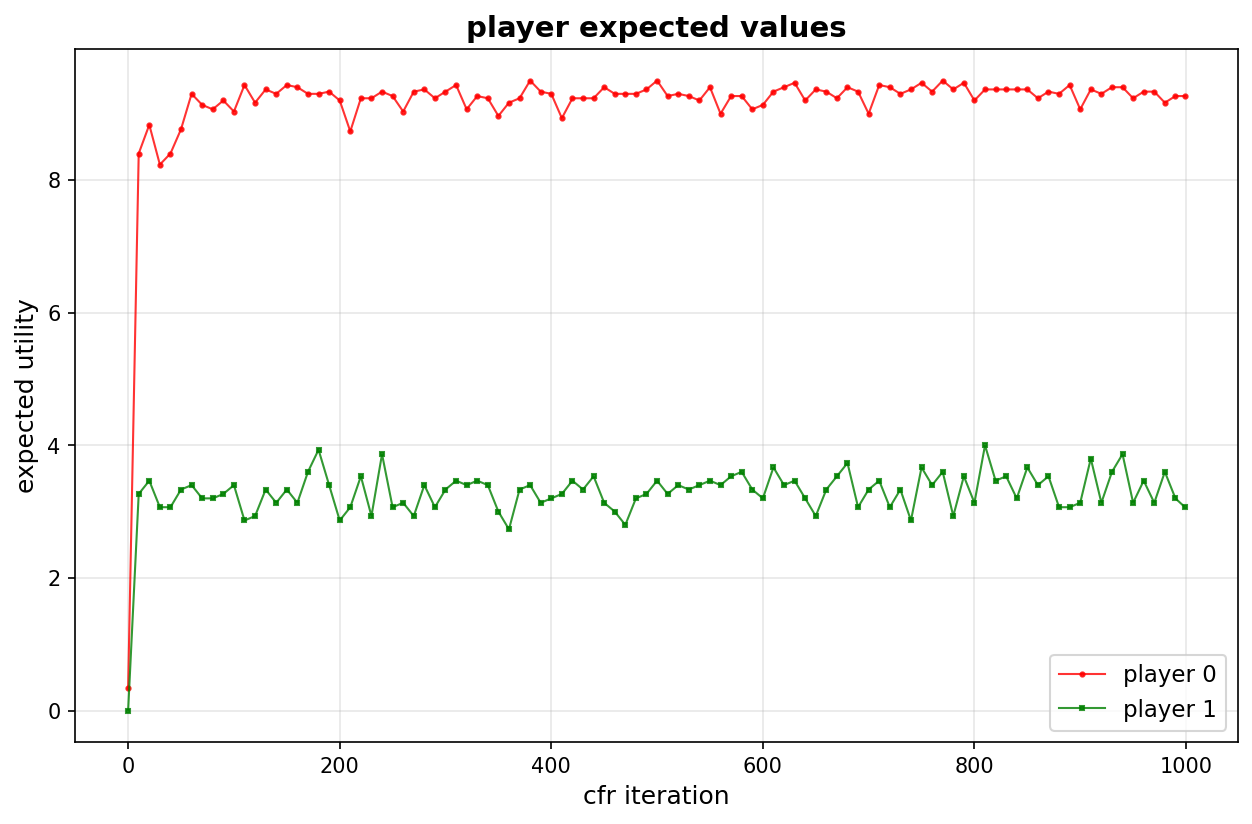
\includegraphics[width=\linewidth]{plots/expected_values/expected_values_cfr.png}
  \caption{CFR}
\end{subfigure}
\begin{subfigure}{0.32\textwidth}
  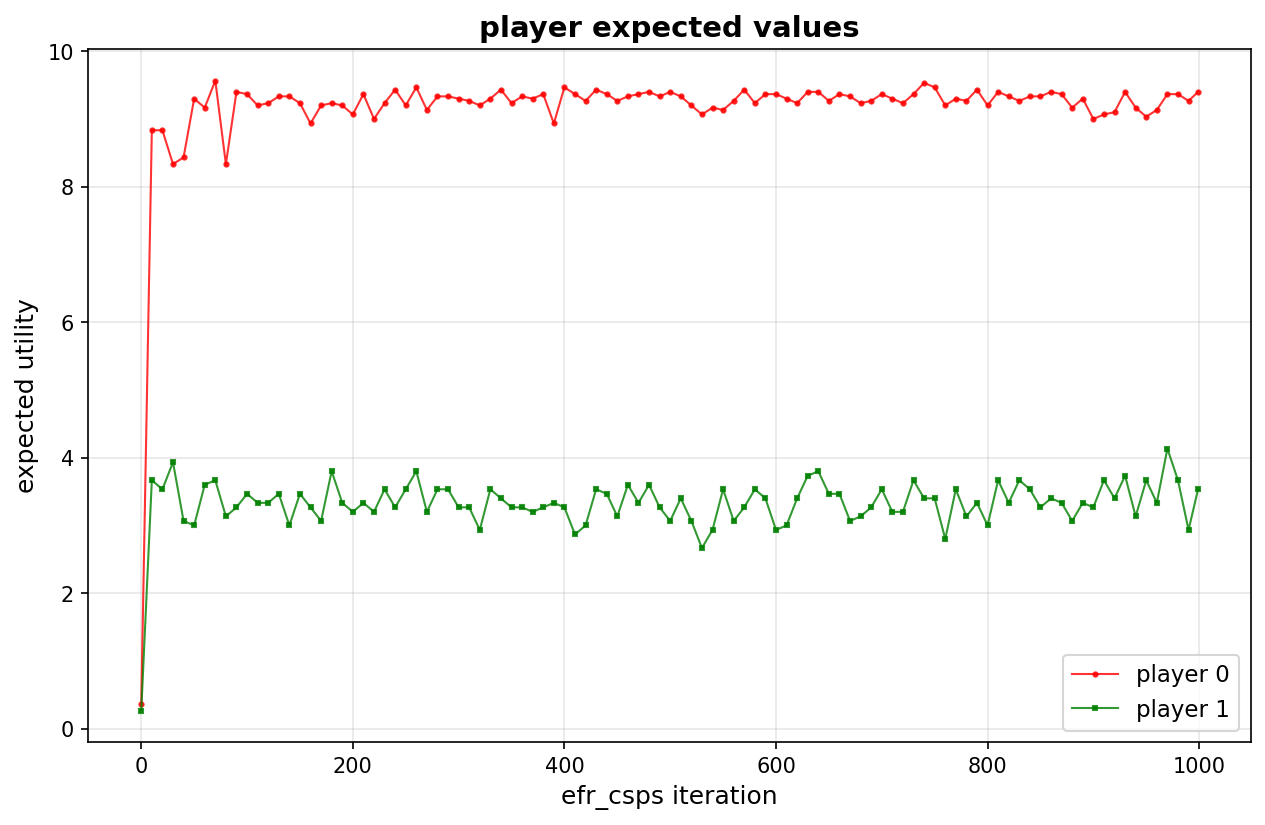
\includegraphics[width=\linewidth]{plots/expected_values/expected_values_csps.png}
  \caption{EFR (CSPS)}
\end{subfigure}
\begin{subfigure}{0.32\textwidth}
  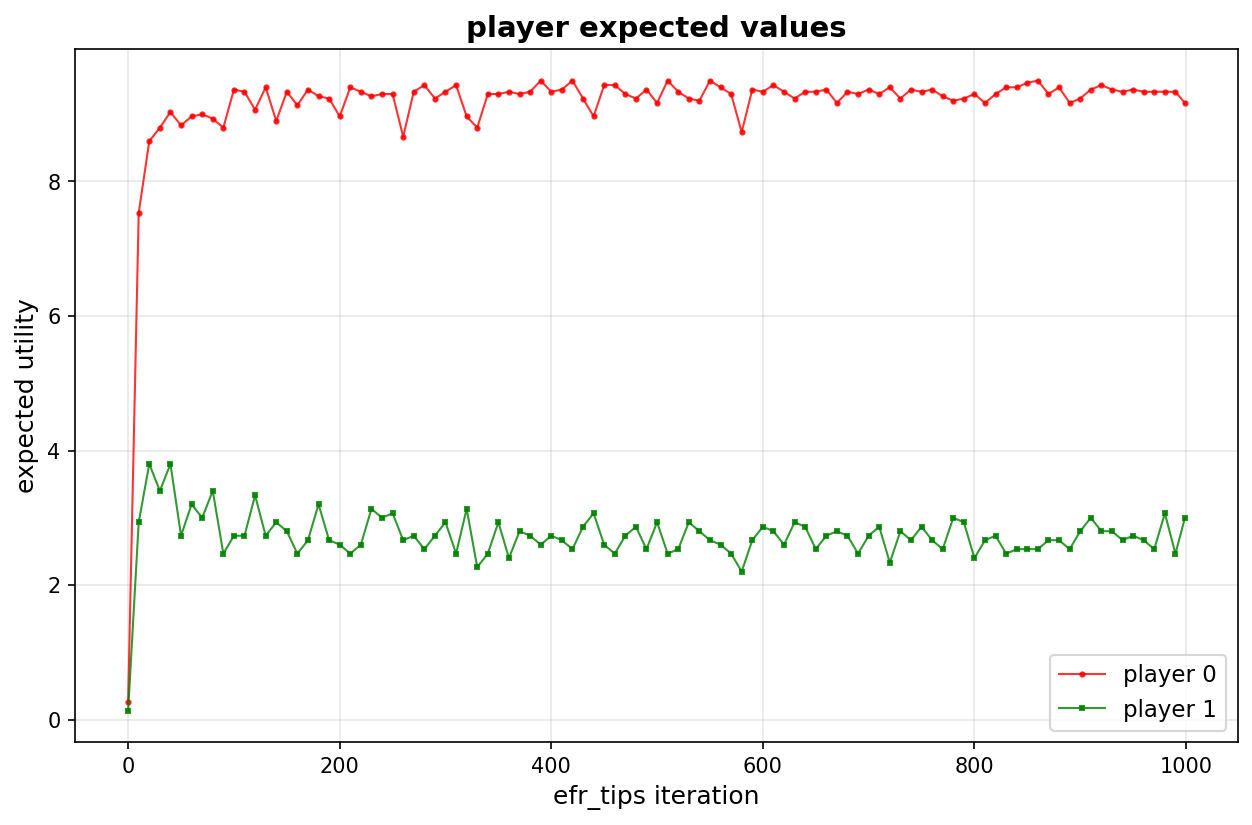
\includegraphics[width=\linewidth]{plots/expected_values/expected_values_tips.png}
  \caption{EFR (TIPS)}
\end{subfigure}
\caption{Expected values for both players over iterations on the 2-turn variant, under CFR, EFR (CSPS), and EFR (TIPS). Player~0 achieves expected values around 9.2 to 9.4 while Player~1 achieves around 3.0 to 3.5, a roughly $3\times$ first-mover advantage.}
\label{fig:asym_2turn}
\end{figure}

This asymmetry is inherent to the game structure rather than an artifact of the learning algorithms. In the 2-turn variant, Player~0 typically achieves expected values around 9.2 to 9.4 while Player~1 achieves around 3.0 to 3.5, giving Player~0 roughly a $3\times$ advantage. The first mover sets the terms of negotiation and can leverage information asymmetries more effectively. All three algorithms converge to similar payoff distributions, suggesting they find equilibria with comparable bargaining outcomes despite their different convergence trajectories.

\subsection{The Reversal: Player 1 Dominates as the Game Lengthens}

To understand how game length affects this asymmetry, we examined CFR convergence on variants with 3 and 4 negotiation turns. Figure~\ref{fig:asym_long} shows expected values for the longer variants.

\begin{figure}[H]
\centering
\begin{subfigure}{0.48\textwidth}
  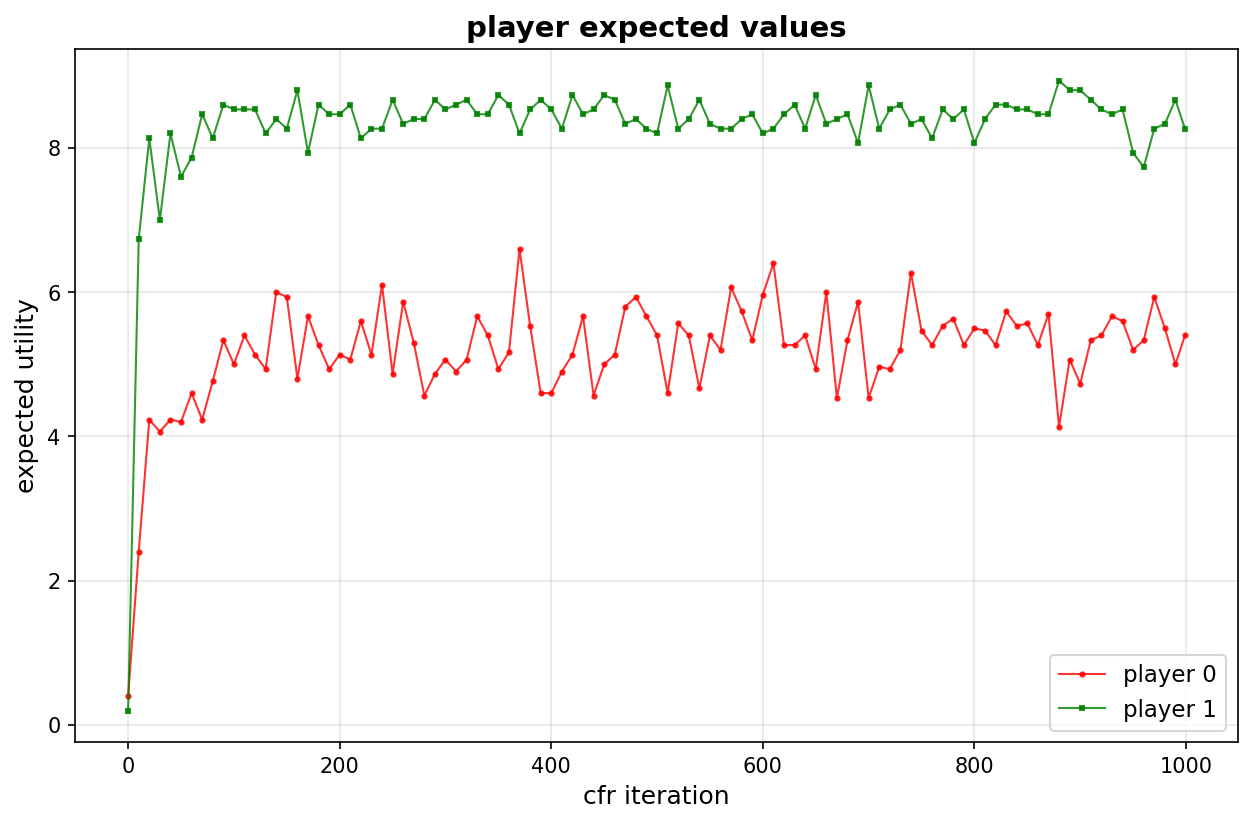
\includegraphics[width=\linewidth]{plots/expected_values/expected_values_3turn.png}
  \caption{CFR on 3-turn game}
\end{subfigure}
\begin{subfigure}{0.48\textwidth}
  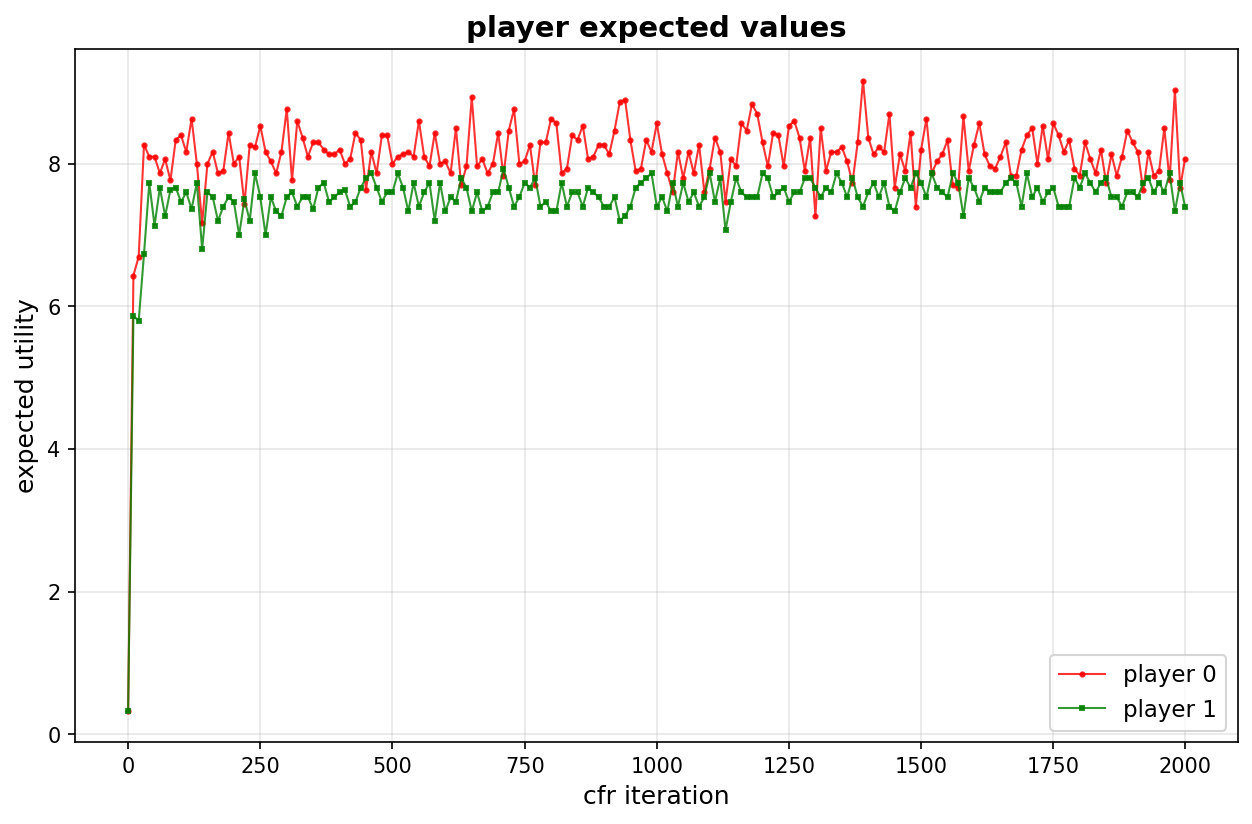
\includegraphics[width=\linewidth]{plots/expected_values/expected_values_4turn.png}
  \caption{CFR on 4-turn game}
\end{subfigure}
\caption{Expected values for both players in extended game variants. The first-mover advantage of Figure~\ref{fig:asym_2turn} not only diminishes but \emph{reverses}: Player~1 dominates the 3-turn variant, and the 4-turn variant is approximately balanced.}
\label{fig:asym_long}
\end{figure}

The pattern is clean: the player asymmetry not only diminishes but \emph{reverses} as the game lengthens. In the 3-turn variant, Player~1 takes the advantage with expected value around 8.27 versus Player~0's 5.4, a complete flip from the 2-turn game. By the 4-turn variant, payoffs become nearly balanced, with Player~0 at 8.07 and Player~1 at 7.4.

\subsection{Discussion}

We interpret this as a first-mover-to-last-mover transition. In the 2-turn variant, Player~0 makes the only proposal (Player~1 can only accept or reject), so Player~0 captures most of the surplus. In the 3-turn variant, Player~1 sees Player~0's opening offer, makes a counter-offer, and Player~0's only remaining choice is to accept Player~1's offer or walk away with zero, so Player~1 captures most of the surplus. In the 4-turn variant, both players get to propose, respond, counter, and respond again; the dynamic becomes more symmetric and the payoff balance follows.

This is a structural finding about the game, not the algorithm: the asymmetry is determined by who gets the \emph{last} concrete proposal, and the symmetry in 4-turn arises only when both players have an equal number of proposals to make. The observation persists across algorithm choices (CFR, EFR-CSPS, EFR-TIPS), which is consistent with all three converging to similar equilibria of the underlying game.

\section{Equilibrium Distance Sweep}
\label{sec:eqdist}

We now turn to the headline algorithm comparison: how do CFR and EFR variants compare in their distance to various equilibrium concepts on \emph{Deal or No Deal}?

\subsection{Equilibrium Concepts}
\label{sec:eqconcepts}

We evaluate algorithms on their ability to minimize distance to six equilibrium concepts:

\begin{itemize}
    \item \textbf{AFCCE (Agent-Form Coarse Correlated Equilibrium).} Coarse correlated equilibrium where deviations are evaluated at the start of the game.
    \item \textbf{AFCE (Agent-Form Correlated Equilibrium).} A refinement of AFCCE where deviations are evaluated at more granular decision points.
    \item \textbf{EFCCE (Extensive-Form Coarse Correlated Equilibrium).} Coarse correlated equilibrium that respects the sequential structure of the extensive-form game.
    \item \textbf{EFCE (Extensive-Form Correlated Equilibrium).} A refinement of EFCCE that requires incentive compatibility at every decision point in the extensive form.
    \item \textbf{CCE / CE (Normal-form Coarse Correlated / Correlated Equilibrium).} The non-extensive-form versions of the same concepts. Earlier text in this thesis incorrectly labeled these ``zero-sum''; \texttt{bargaining\_small} is general-sum, but the CCE/CE distance metrics are well-defined on any game.
\end{itemize}

\subsection{Hypotheses}
\label{sec:hypotheses}

Morrill et al.~(2021b) establish the deviation hierarchy
\[
\text{BHV} \succ \text{TIPS} \succ \{\text{CSPS, CFPS}\} \succ \text{BPS} \succ \{\text{action, causal, counterfactual}\} \succ \text{external},
\]
where stronger deviation sets subsume weaker ones (under observable-sequential rationality in several cases) and are therefore expected to produce tighter equilibrium distance under their corresponding equilibrium concepts. Their own empirical finding is that TIPS and CSPS often perform nearly as well as BHV in games of moderate length, while BHV pays the highest computational cost. Our hypotheses follow from this hierarchy paired with the structure of each equilibrium concept.

\begin{enumerate}
    \item \textbf{AFCCE.} EFR with (blind) action deviations should minimize AFCCE distance best, since AFCCE's deviation class is exactly the blind action deviations.
    \item \textbf{AFCE.} EFR with informed action deviations should minimize AFCE distance best, mirroring (1) under internal rather than external transformations.
    \item \textbf{EFCCE ordering.} BHV $\succ$ TIPS $\succ$ CSPS $\succ$ CFR. Within the ``coarse'' family, the deviation hierarchy should reproduce on EFCCE distance.
    \item \textbf{EFCE ordering.} BHV$_\text{in}$ $\succ$ TIPS$_\text{in}$ $\succ$ CFPS$_\text{in}$ $\succ$ CFR$_\text{in}$. Internal-regret variants correspond to the informed-deviation versions of the hierarchy.
    \item \textbf{TIPS $\approx$ BHV at moderate cost.} Consistent with Morrill et al., we expect TIPS to come close to BHV's final equilibrium distance while being cheaper per iteration.
    \item \textbf{Game-length scaling.} As \texttt{max\_turns} increases from 2 to 4, the gap between the weakest and strongest deviation types should widen, because deeper games admit more types of profitable single-target deviations.
\end{enumerate}

\subsection{Experimental Protocol}

\paragraph{Game.} \texttt{bargaining\_small} with \texttt{max\_turns} $\in \{2, 3, 4\}$. Each turn count is run as its own sweep. CCE/CE distances are reported alongside AFCCE/AFCE/EFCCE/EFCE for completeness, with the reminder that this is a general-sum game.

\paragraph{Algorithm $\times$ equilibrium matrix.} Table~\ref{tab:matrix} lists the runs. Each cell is executed once per \texttt{max\_turns} value at \texttt{random\_seed=0}. Two algorithms named in the original experiment plan, \texttt{EFR\_BPS} and the external-regret variant of \texttt{EFR\_CFPS}, are not implemented in the C++ binary's deviation-set switch and are dropped from this sweep; they would require a small C++ extension to add.

\begin{table}[H]
\centering
\caption{Algorithm $\times$ equilibrium matrix. \checkmark denotes an included run; an empty cell means the (algorithm, equilibrium) pair is not in the run matrix.}
\label{tab:matrix}
\begin{tabular}{lcccccc}
\toprule
Algorithm & AFCCE & AFCE & EFCCE & EFCE & CCE & CE \\
\midrule
CFR                 & \checkmark &            & \checkmark &            & \checkmark & \checkmark \\
CFR\_in             &            & \checkmark &            & \checkmark & \checkmark & \checkmark \\
EFR\_ACT            & \checkmark &            &            &            &            &            \\
EFR\_ACT\_in        &            & \checkmark &            &            &            &            \\
EFR\_CFPS\_in       &            &            &            & \checkmark &            &            \\
EFR\_CSPS           &            &            & \checkmark &            &            &            \\
EFR\_TIPS           &            &            & \checkmark &            &            &            \\
EFR\_TIPS\_in       &            &            &            & \checkmark &            &            \\
EFR\_BHV            &            &            & \checkmark &            &            &            \\
EFR\_BHV\_in        &            &            &            & \checkmark &            &            \\
\bottomrule
\end{tabular}
\end{table}

\paragraph{Training and reporting.} The 2-turn sweep is run for 1{,}000 iterations with reporting every 50 iterations. The 3-turn sweep is run for 100 iterations with reporting every 10 iterations (10 points along each convergence curve). The shorter budget at depth is chosen so the snapshot is taken before the empirical correlation device for the most expressive deviation sets (CSPS, TIPS, BHV) enters the oscillation regime described in \S\ref{sec:eqdist_disc}. All distances are computed exactly (no Monte Carlo distance approximation). Correlation-device sampling uses outcome sampling with \texttt{num\_samples}$=10$ per iteration.

\paragraph{Seeds.} The 2-turn sweep uses \texttt{random\_seed=0}; the 3-turn sweep uses \texttt{random\_seed=2}. Plots show the raw curve without confidence bands; tables report final-iteration distances directly.

\paragraph{Compute.} 16 (algorithm, equilibrium) pairs are run per turn count, 8 in parallel on a 10-core arm64 Mac. Per-run wall-clock time is dominated by the equilibrium-distance computation: the 2-turn sweep runs in roughly 30 minutes; the 3-turn sweep at 100 iterations runs in roughly 5 minutes.

\subsection{Results: 2-Turn Variant}
\label{sec:results_t2}

The full 16-run sweep on \texttt{max\_turns}$=2$ has completed. Table~\ref{tab:t2_results} reports the final-iteration distance for each (algorithm, equilibrium) cell, and Figure~\ref{fig:t2_curves} plots the convergence curves.

\begin{table}[H]
\centering
\caption{Final-iteration equilibrium distance on \texttt{max\_turns}$=2$ after 1{,}000 iterations. Numerical zeros (essentially machine epsilon) are reported in scientific notation. Empty cells are not in the run matrix.}
\label{tab:t2_results}
\begin{tabular}{lcccccc}
\toprule
Algorithm & AFCCE & AFCE & EFCCE & EFCE & CCE & CE \\
\midrule
CFR             & 2.2e-15 &         & 5.1e-15 &         & 0.013   & 0 \\
CFR\_in         &         & 0.065   &         & 0.131   & 5.0e-08 & 0.095 \\
EFR\_ACT        & 0       &         &         &         &         & \\
EFR\_ACT\_in    &         & 1.2e-14 &         &         &         & \\
EFR\_CSPS       &         &         & 2.0e-14 &         &         & \\
EFR\_TIPS       &         &         & 0.010   &         &         & \\
EFR\_BHV        &         &         & 0.038   &         &         & \\
EFR\_CFPS\_in   &         &         &         & 1.0e-05 &         & \\
EFR\_TIPS\_in   &         &         &         & 0.032   &         & \\
EFR\_BHV\_in    &         &         &         & 9.0e-12 &         & \\
\bottomrule
\end{tabular}
\end{table}

\begin{figure}[H]
\centering
\begin{subfigure}{0.32\textwidth}
  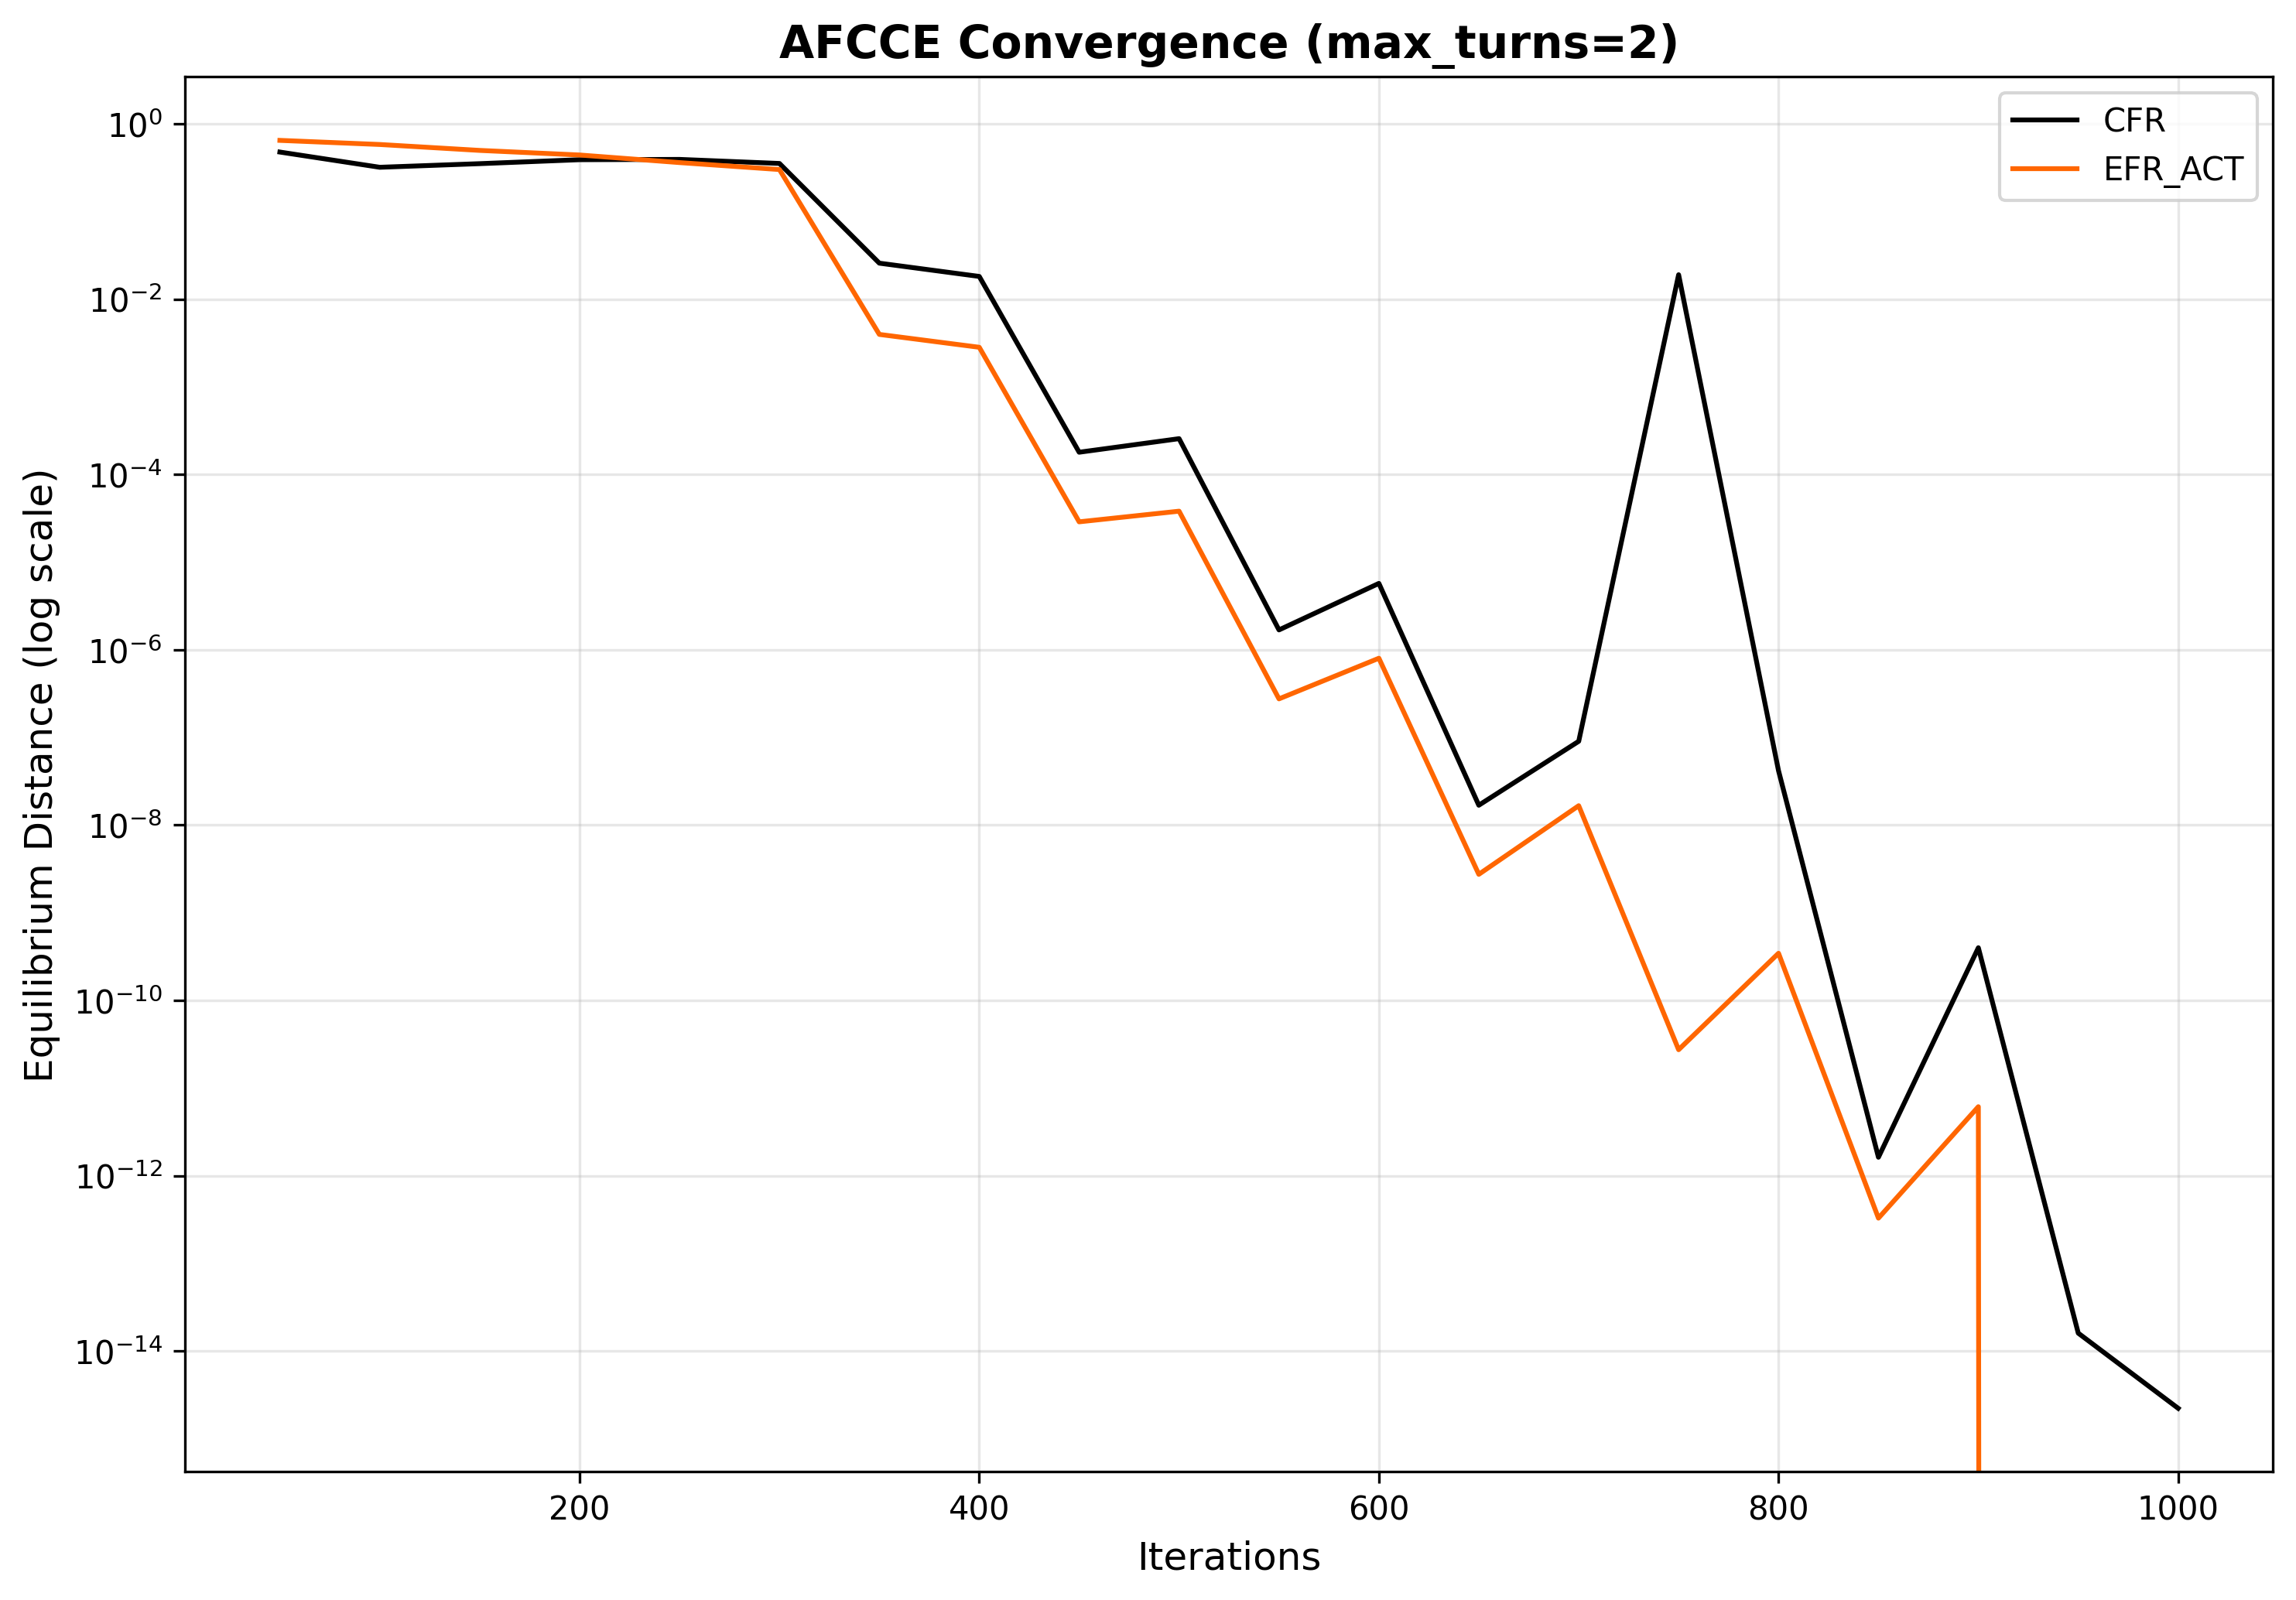
\includegraphics[width=\linewidth]{plots/eq_dist/t2_afcce_convergence.png}
  \caption{AFCCE}
\end{subfigure}
\begin{subfigure}{0.32\textwidth}
  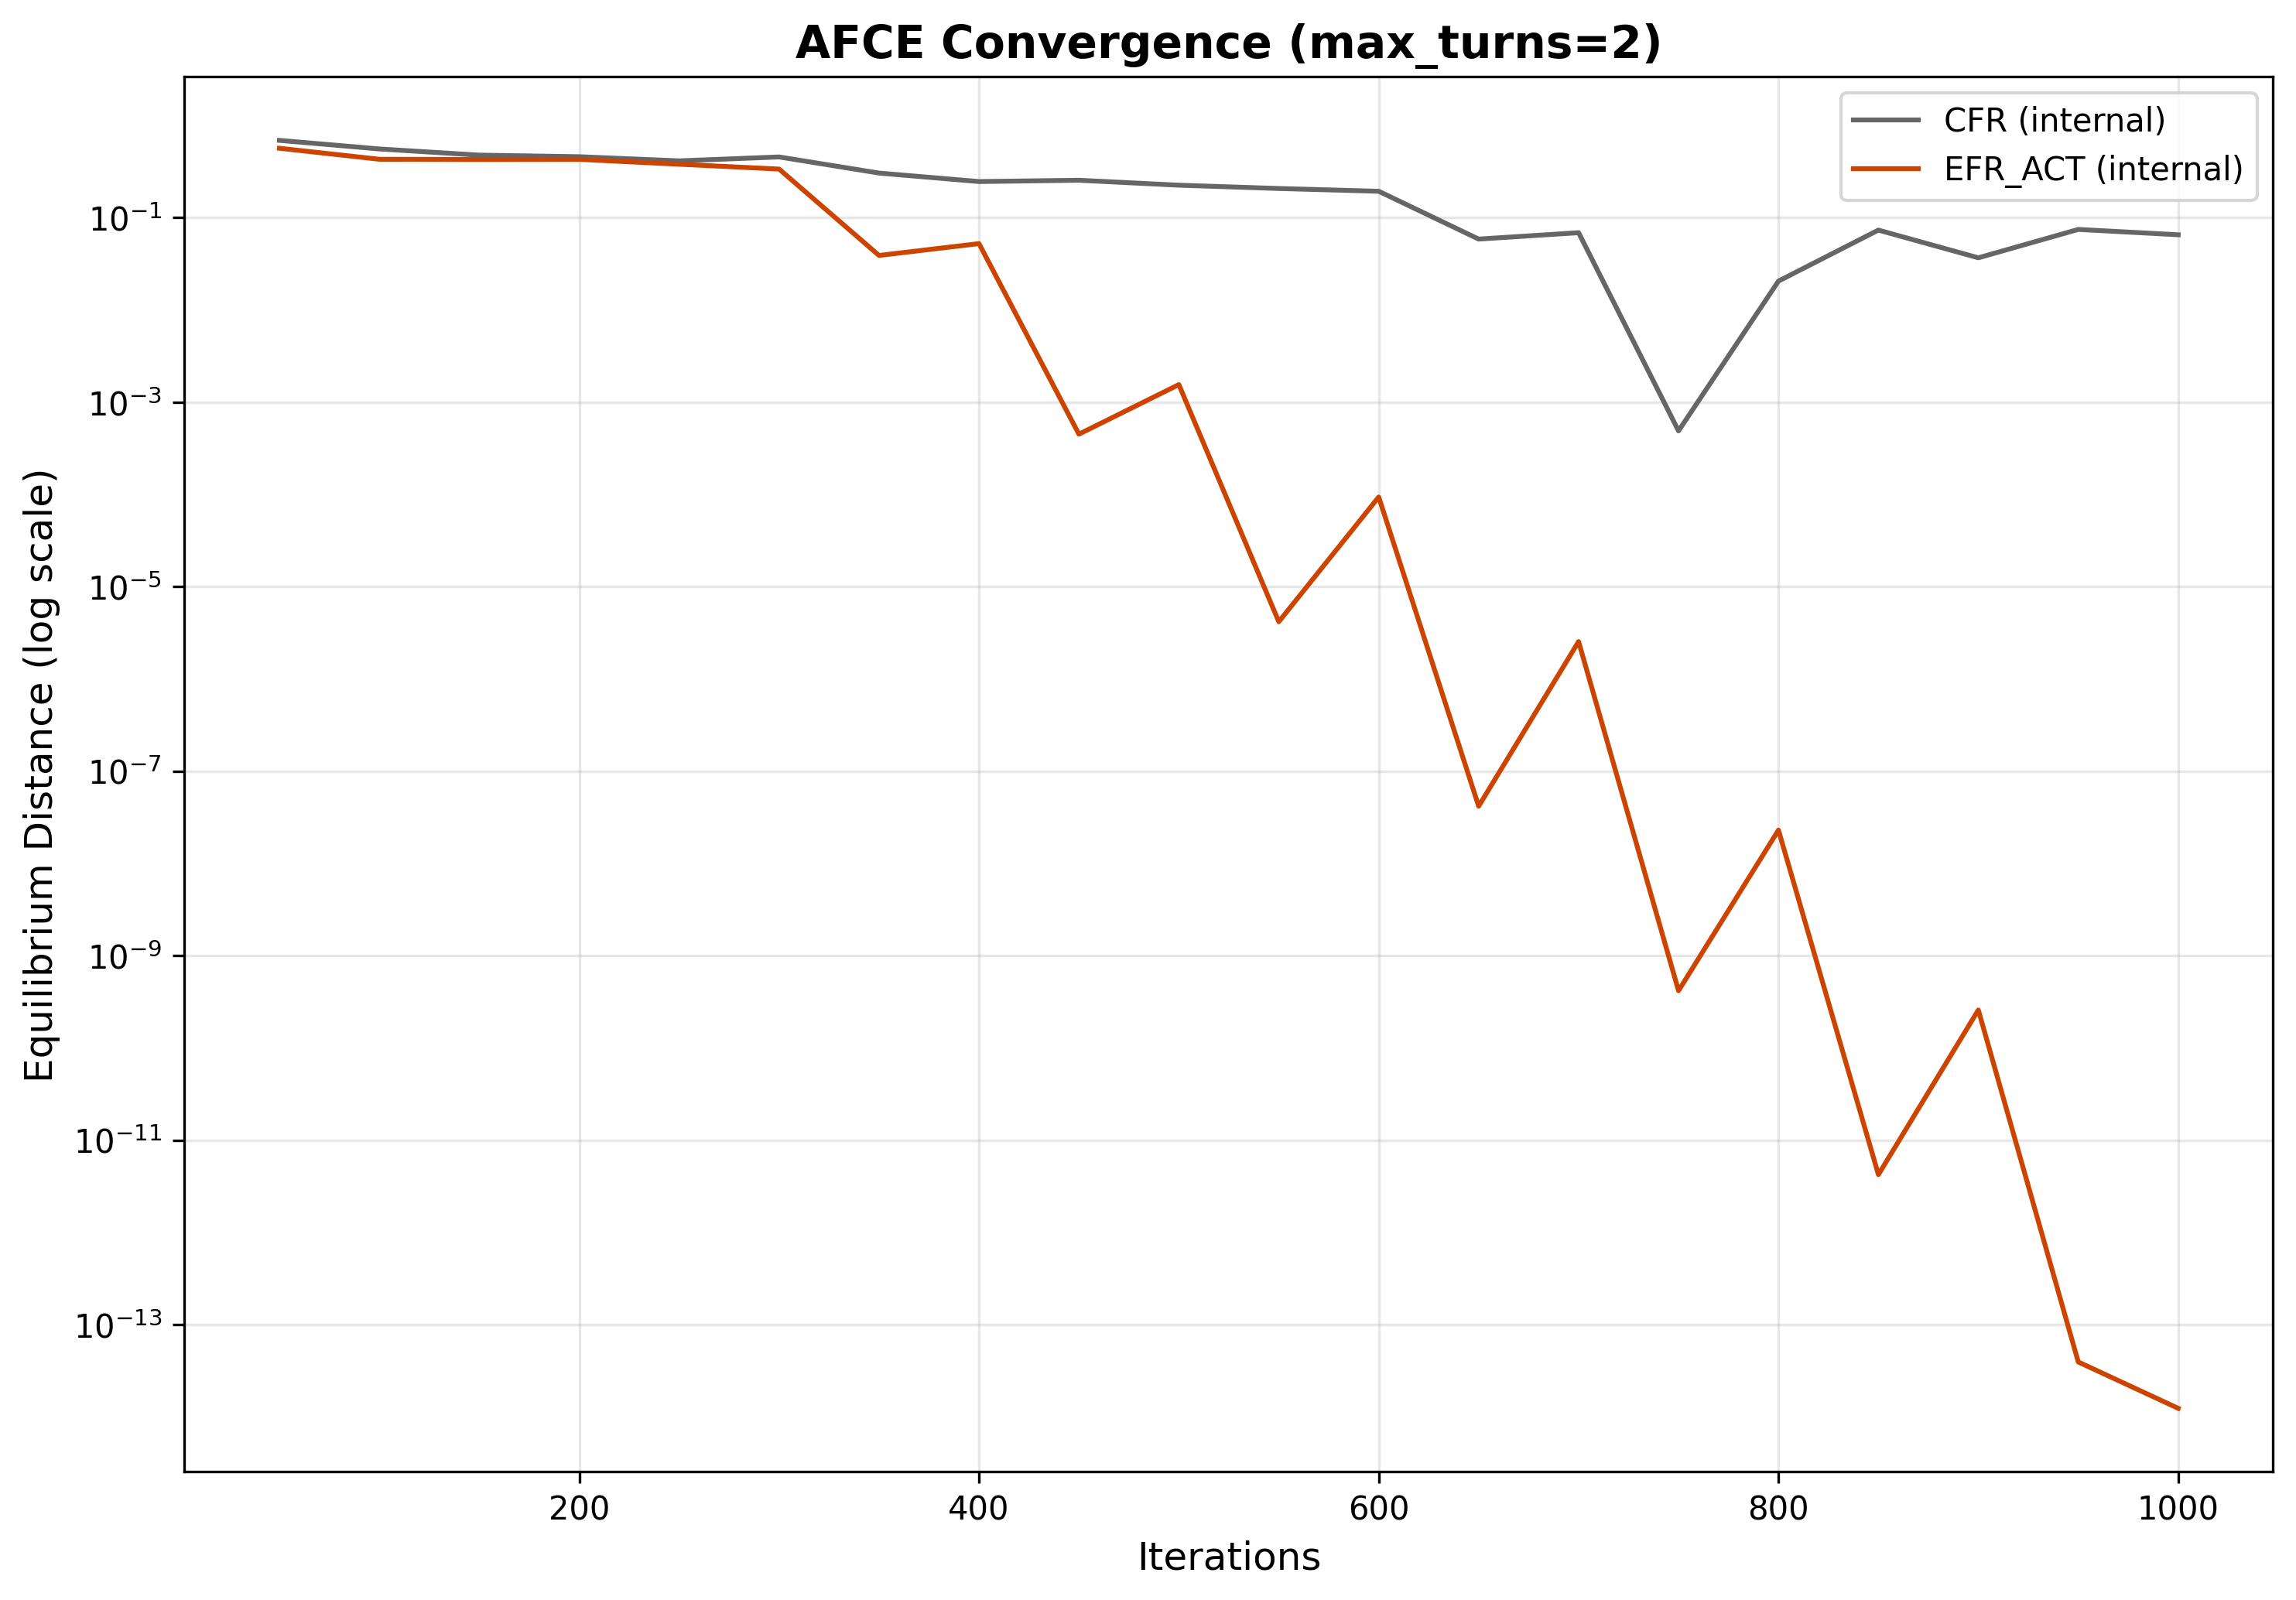
\includegraphics[width=\linewidth]{plots/eq_dist/t2_afce_convergence.png}
  \caption{AFCE}
\end{subfigure}
\begin{subfigure}{0.32\textwidth}
  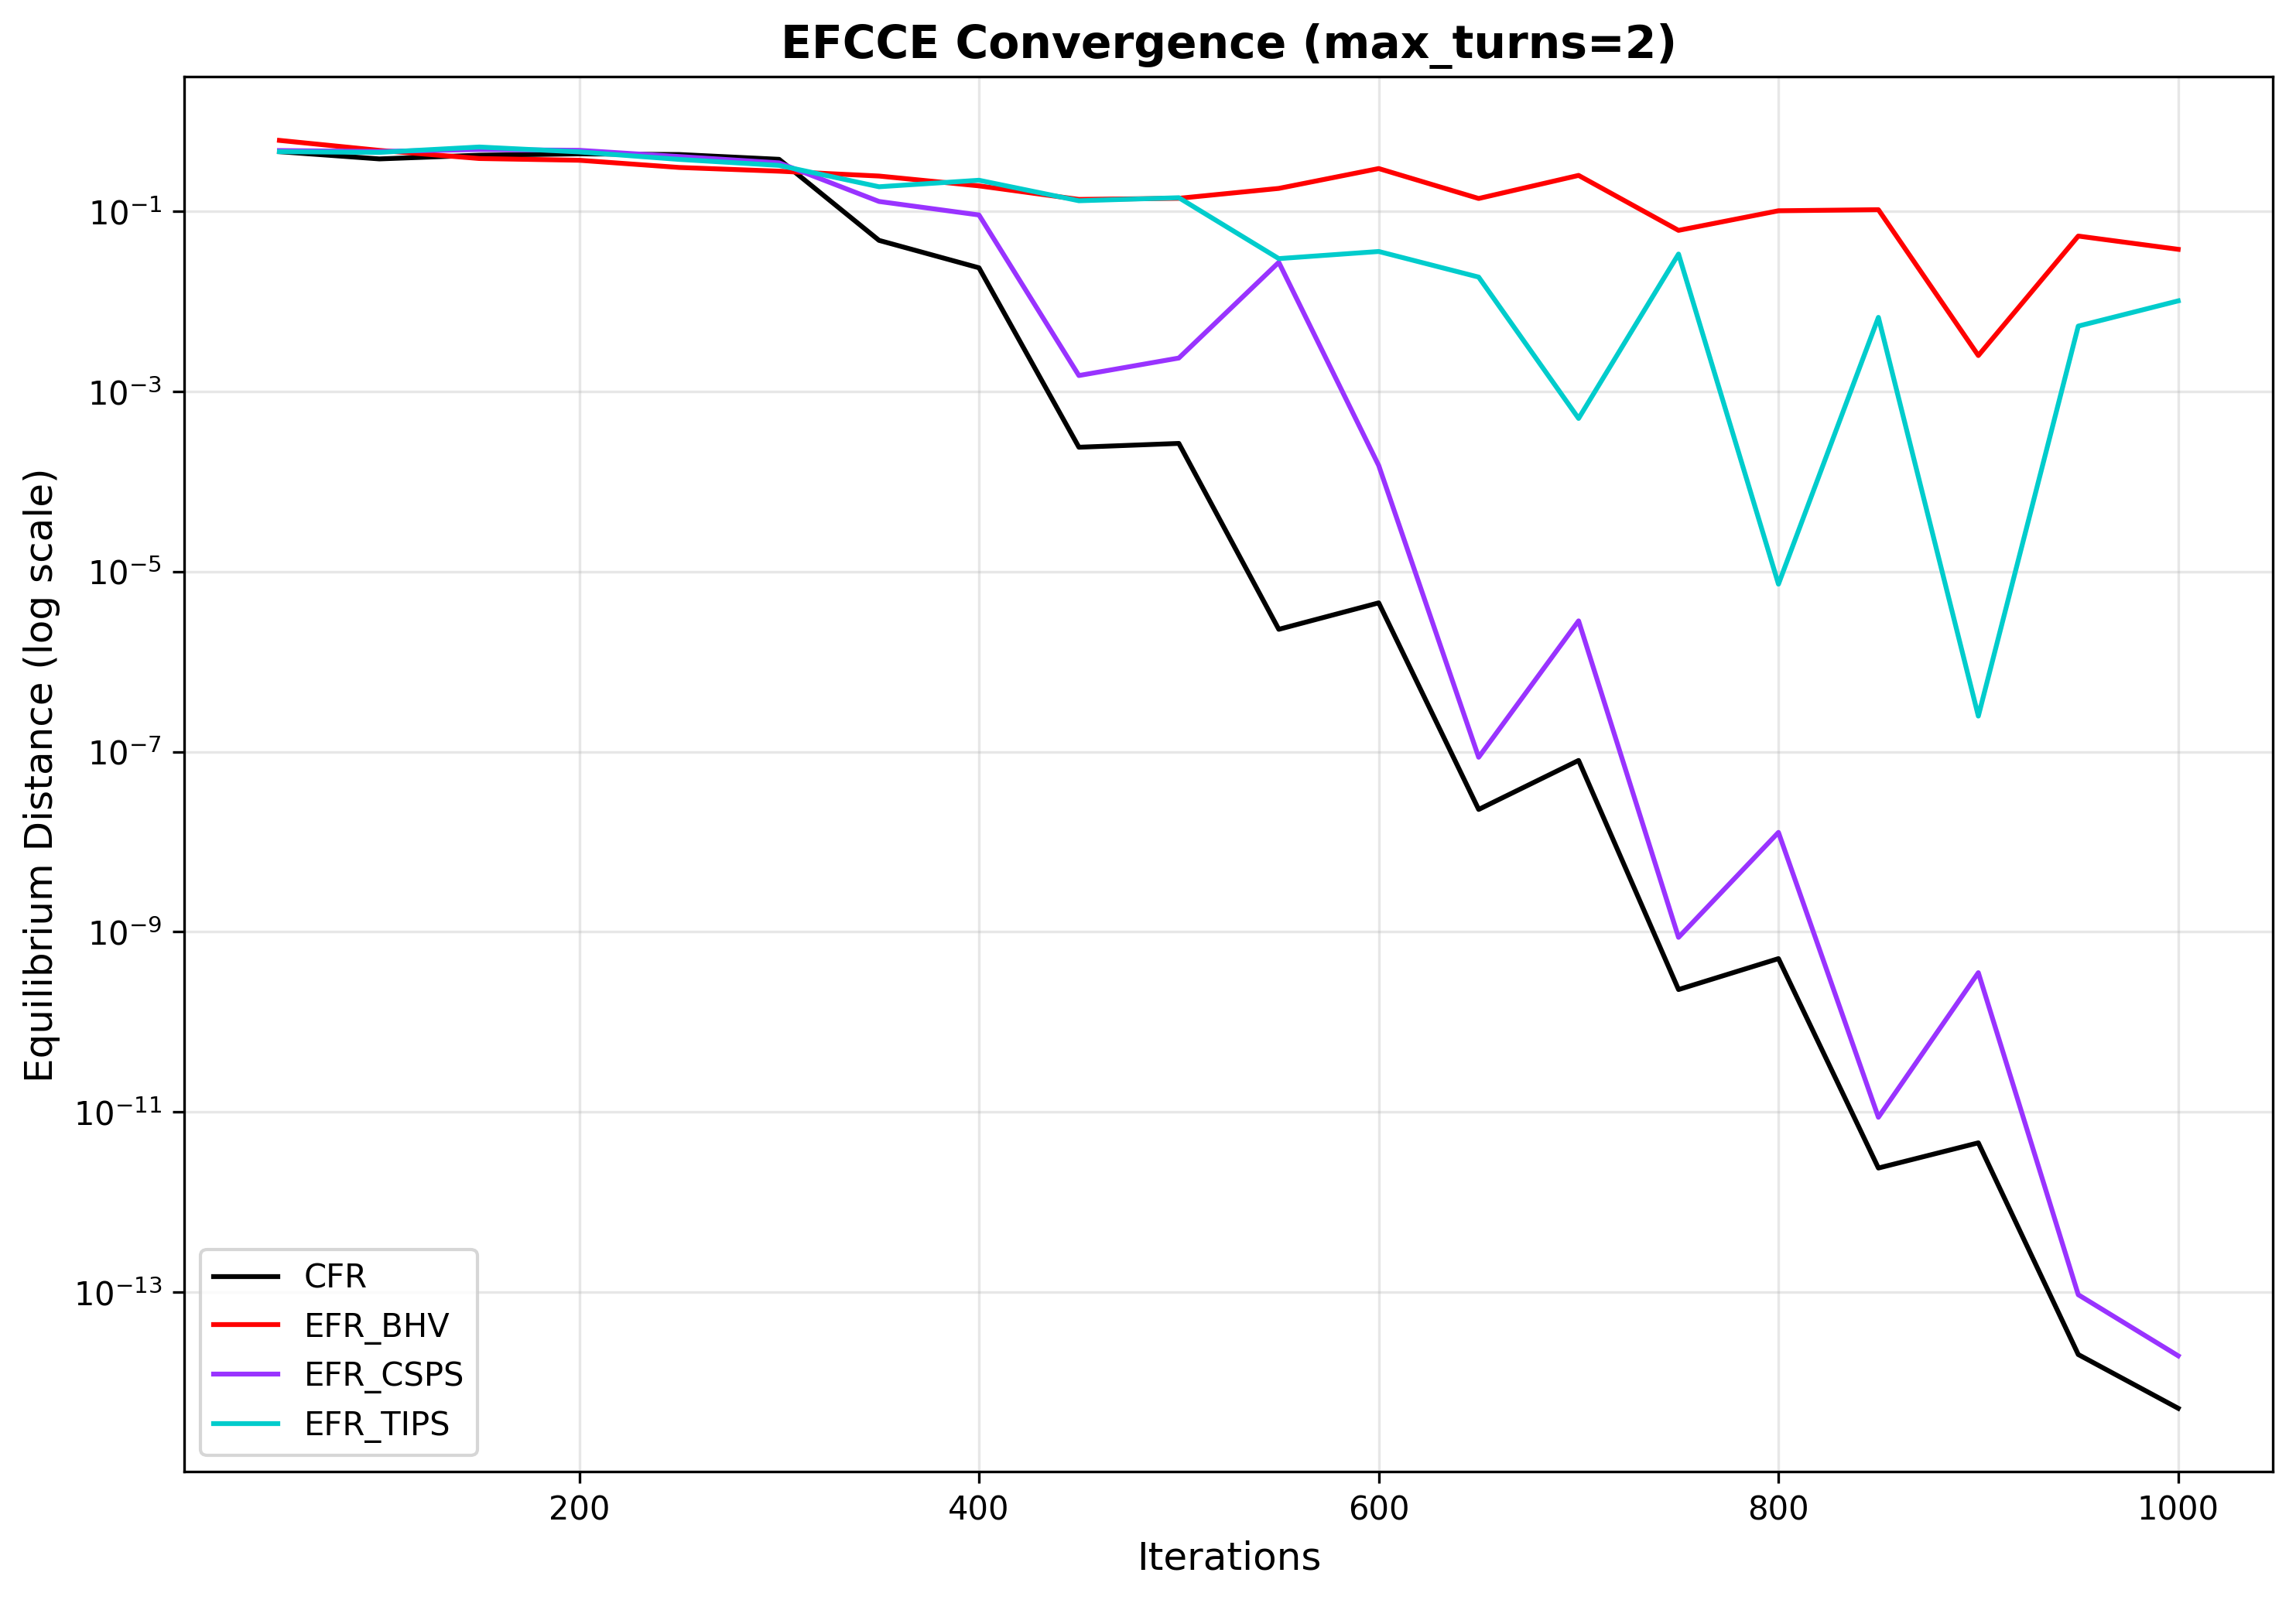
\includegraphics[width=\linewidth]{plots/eq_dist/t2_efcce_convergence.png}
  \caption{EFCCE}
\end{subfigure}

\begin{subfigure}{0.32\textwidth}
  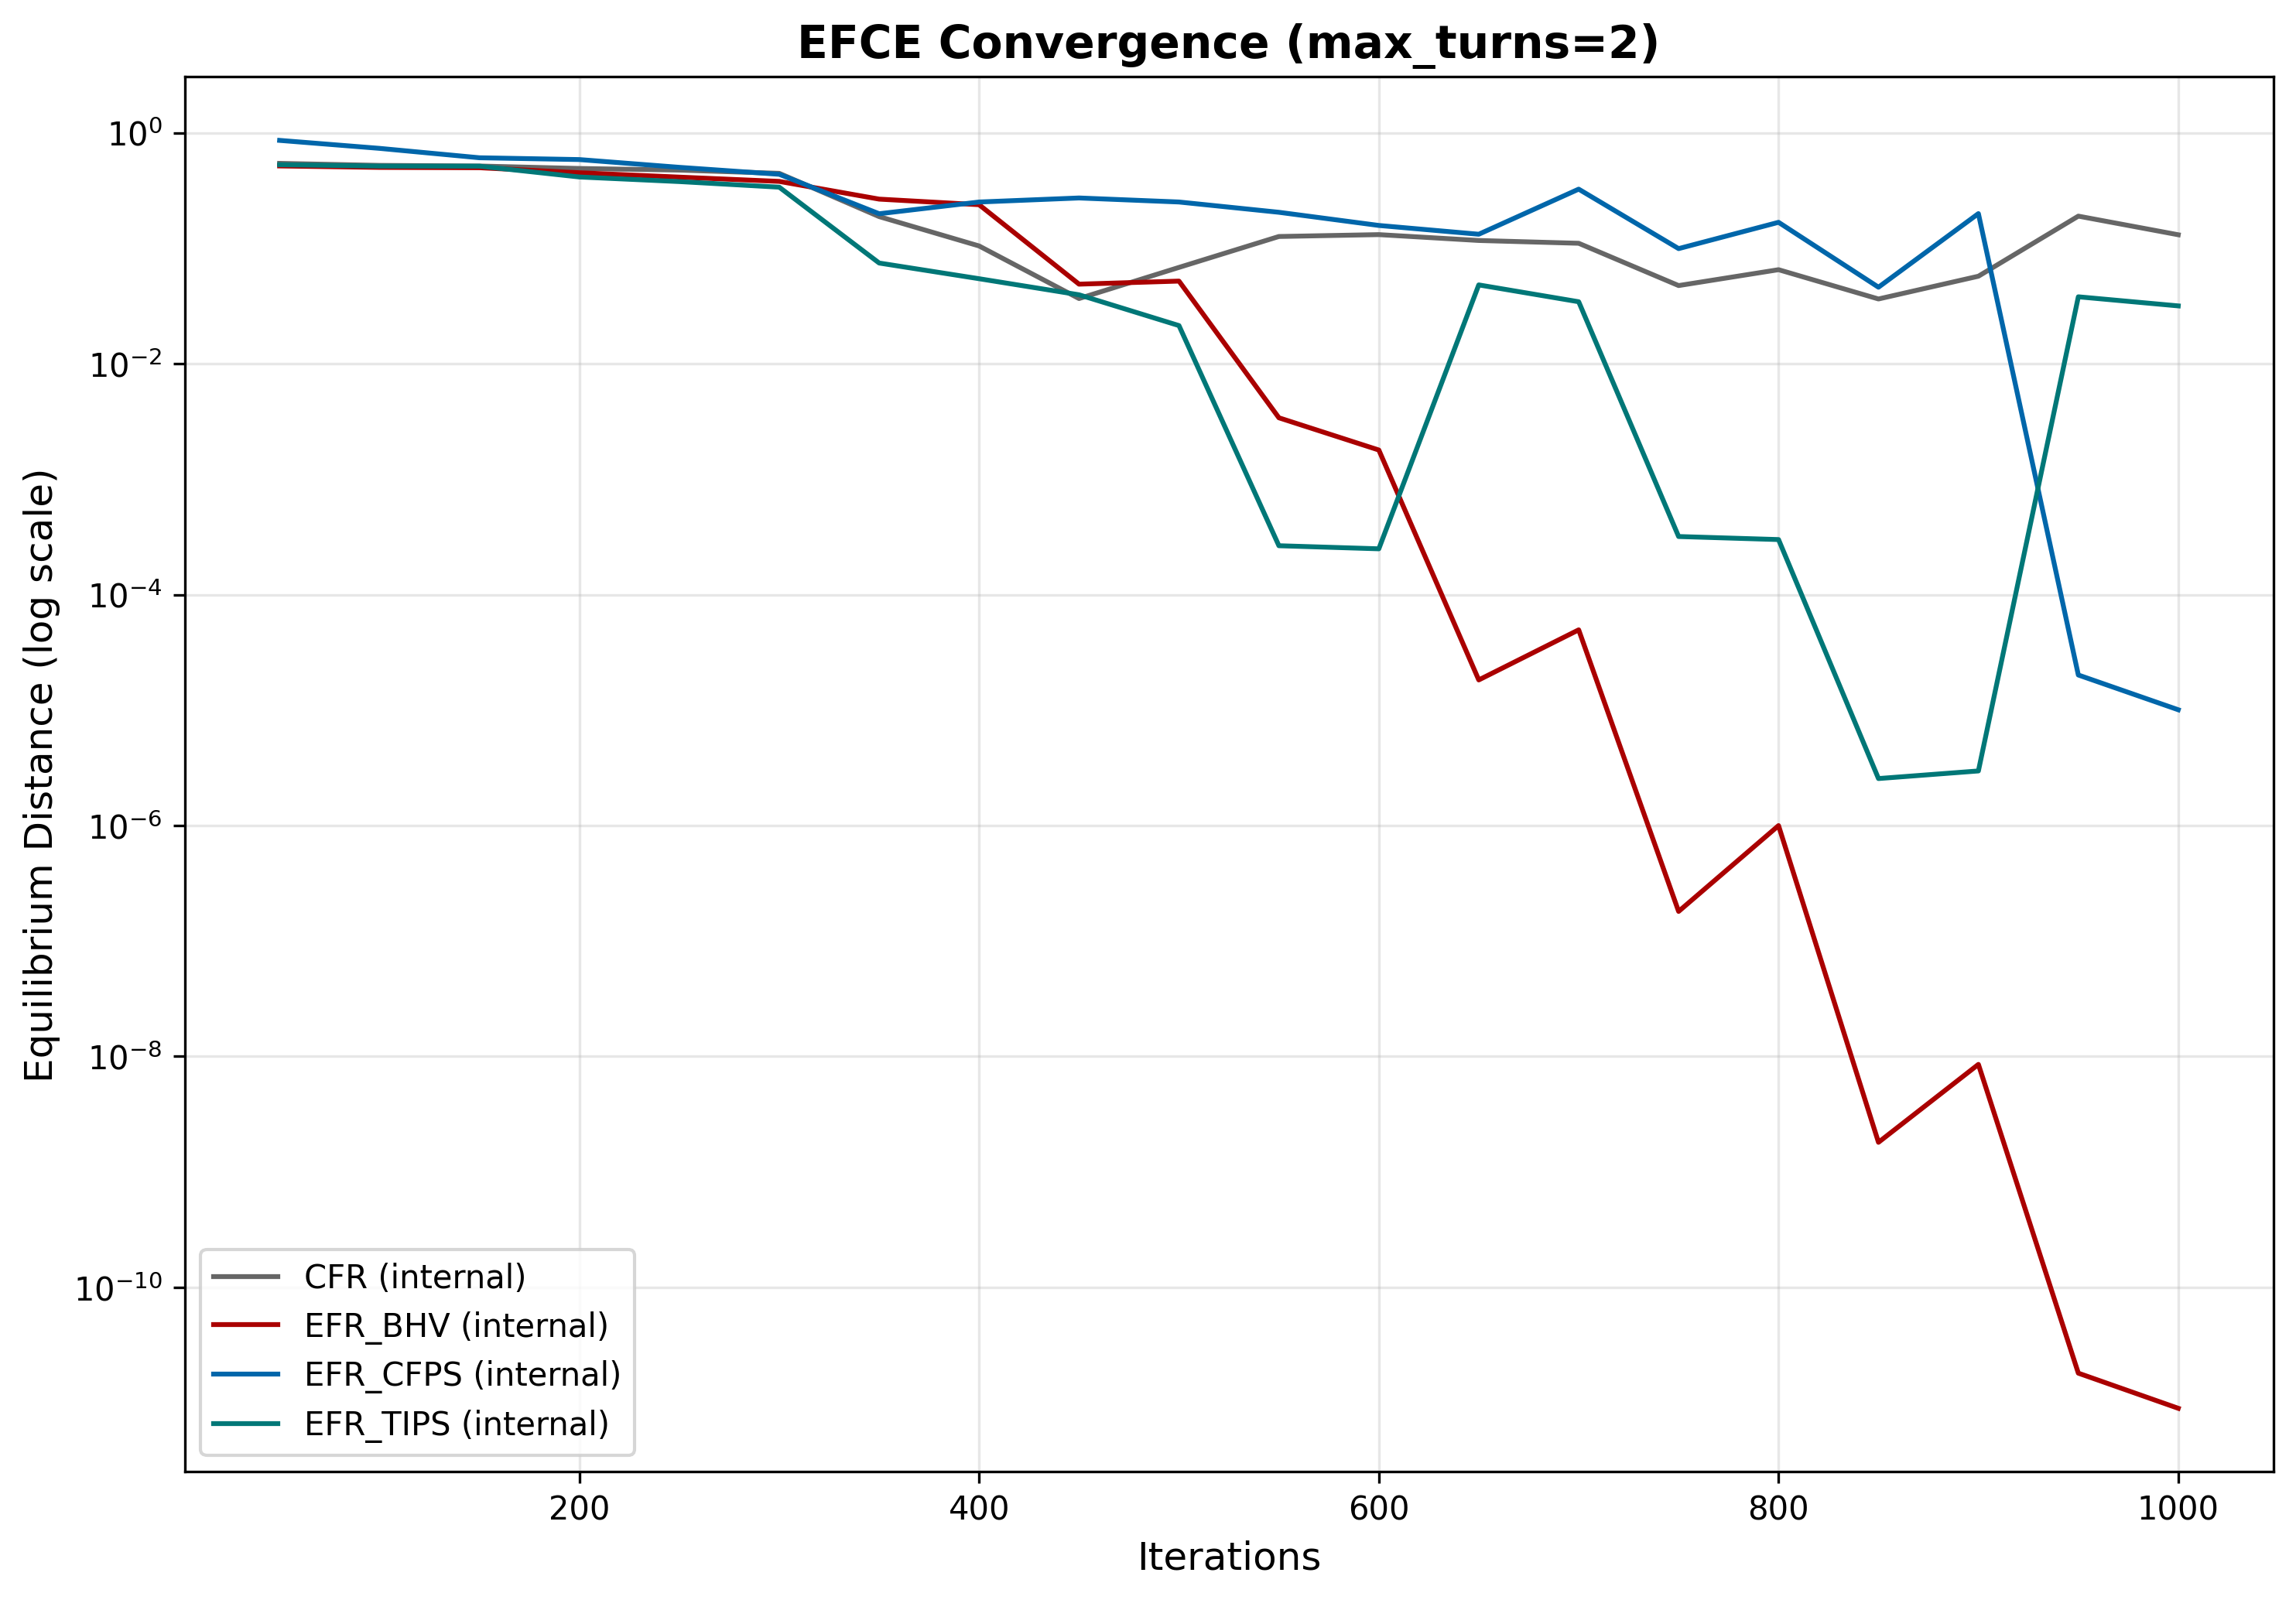
\includegraphics[width=\linewidth]{plots/eq_dist/t2_efce_convergence.png}
  \caption{EFCE}
\end{subfigure}
\begin{subfigure}{0.32\textwidth}
  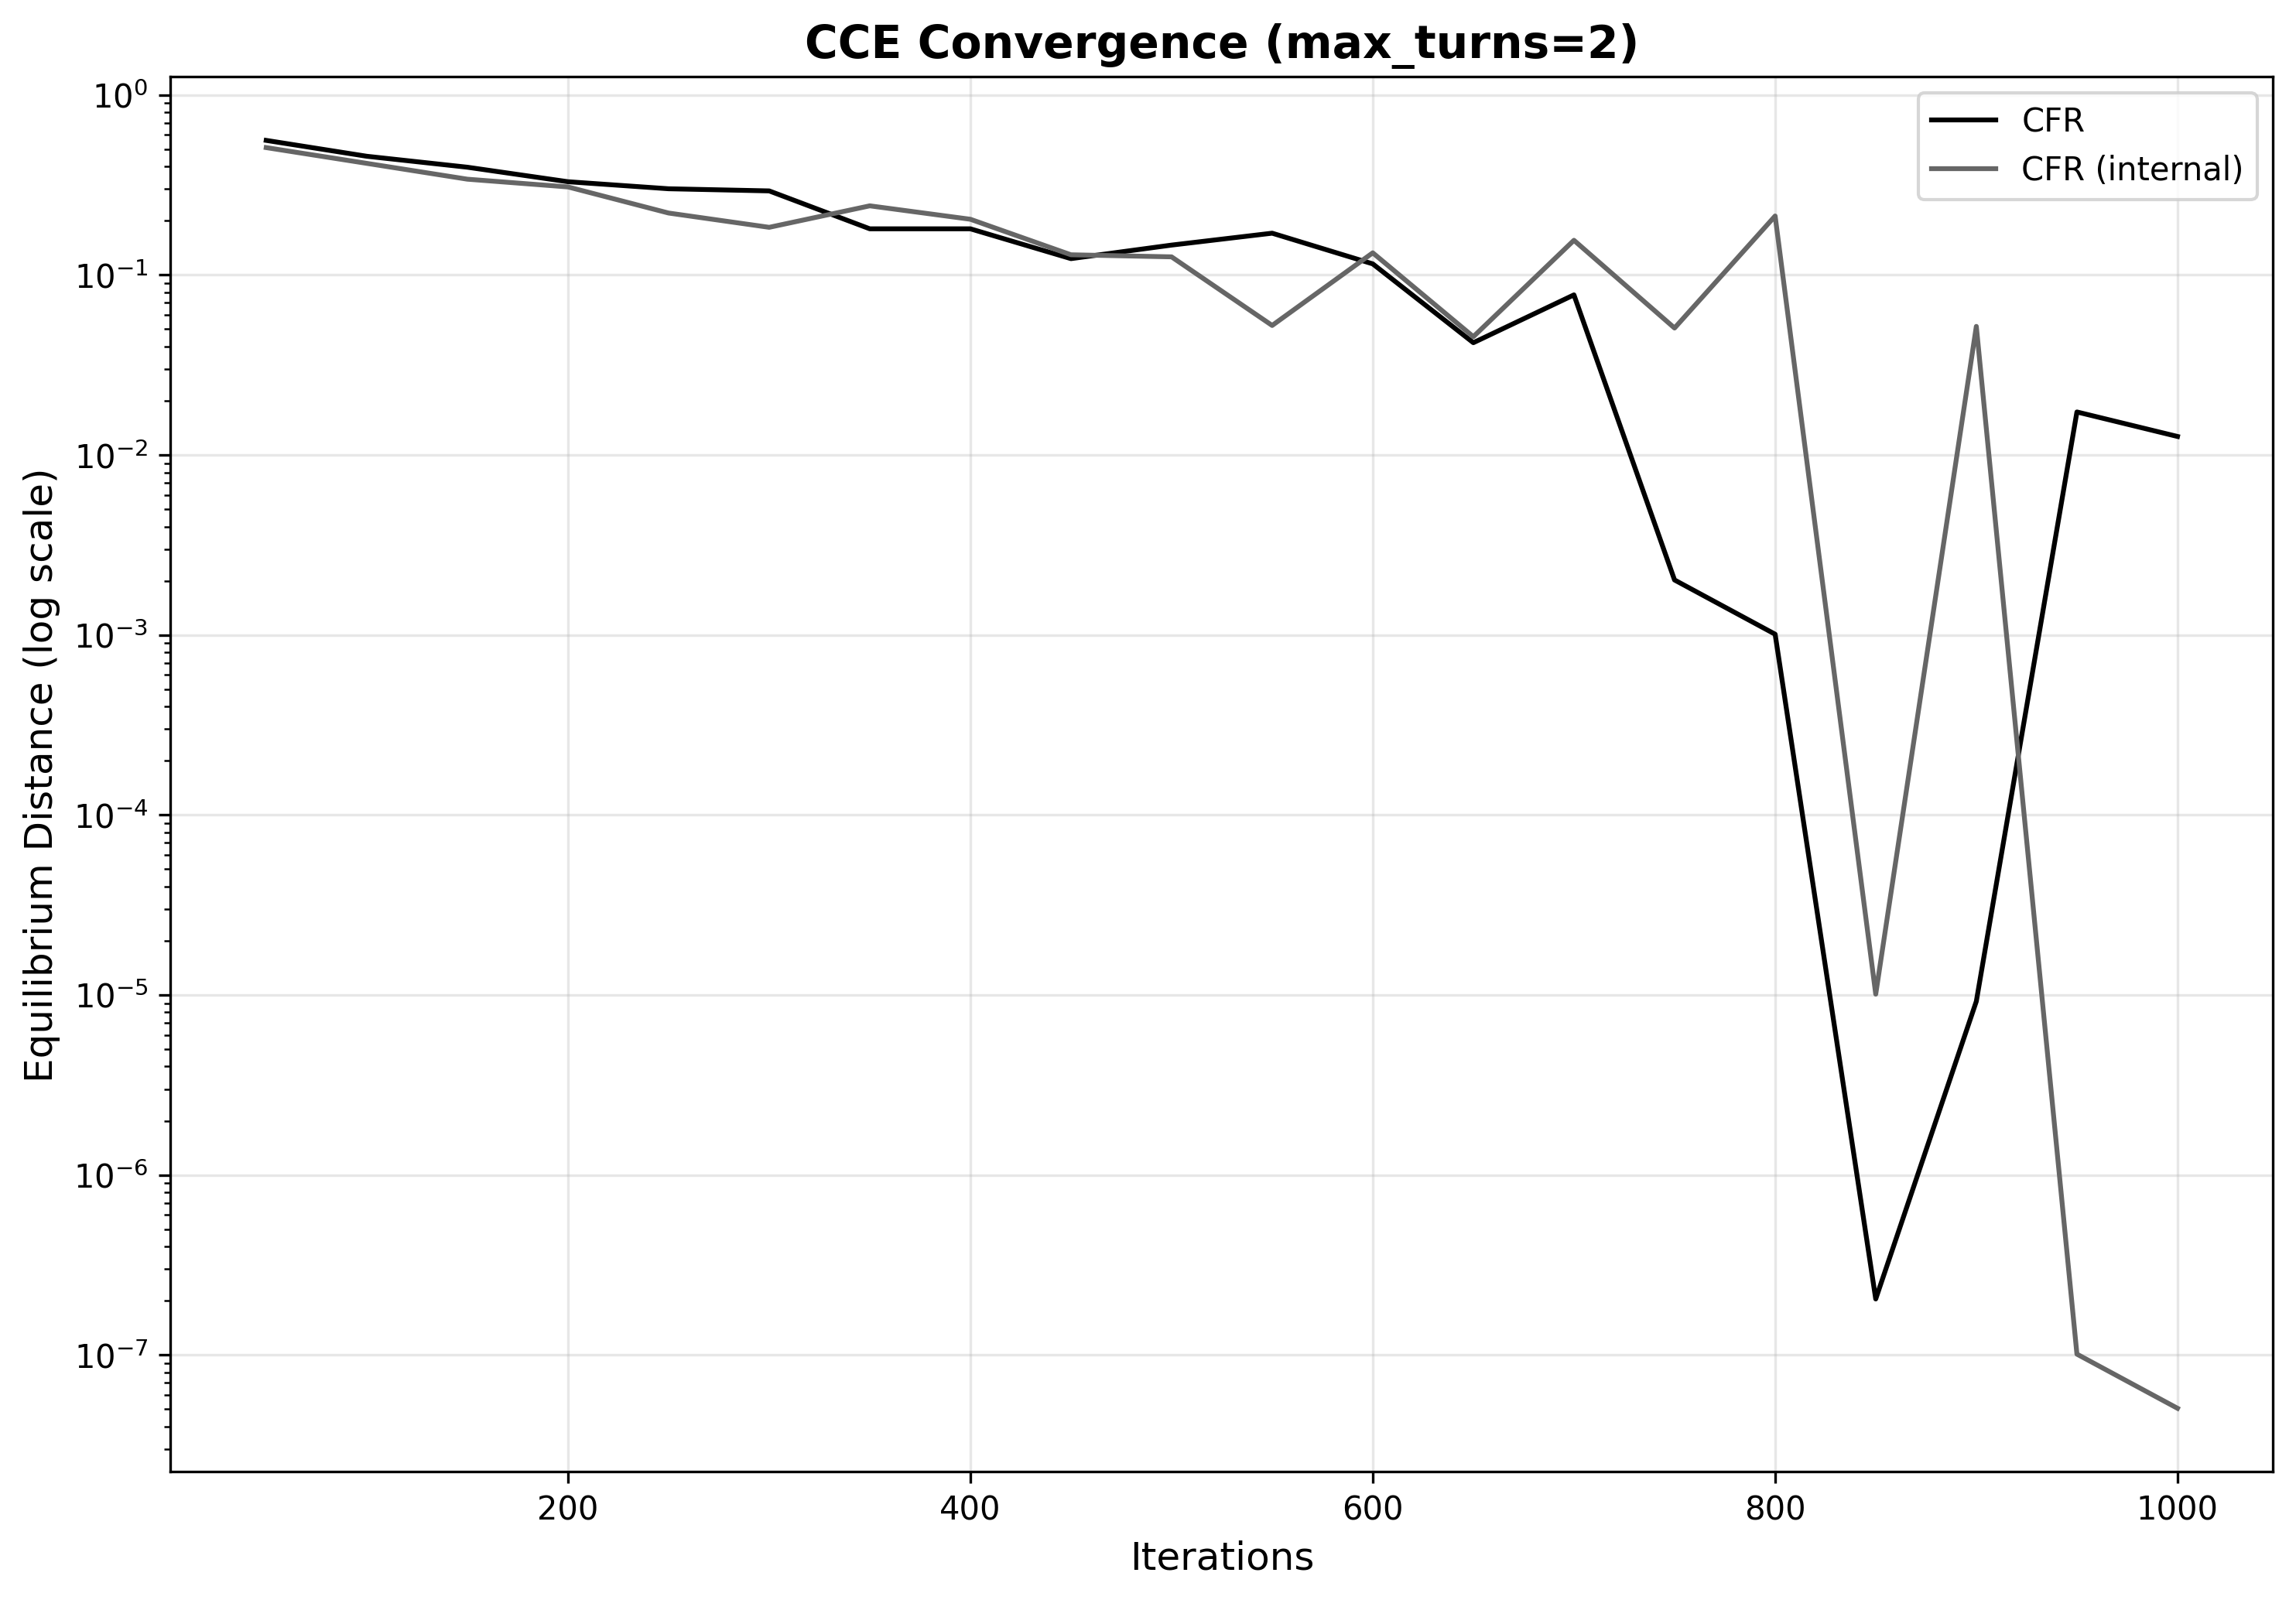
\includegraphics[width=\linewidth]{plots/eq_dist/t2_cce_convergence.png}
  \caption{CCE}
\end{subfigure}
\begin{subfigure}{0.32\textwidth}
  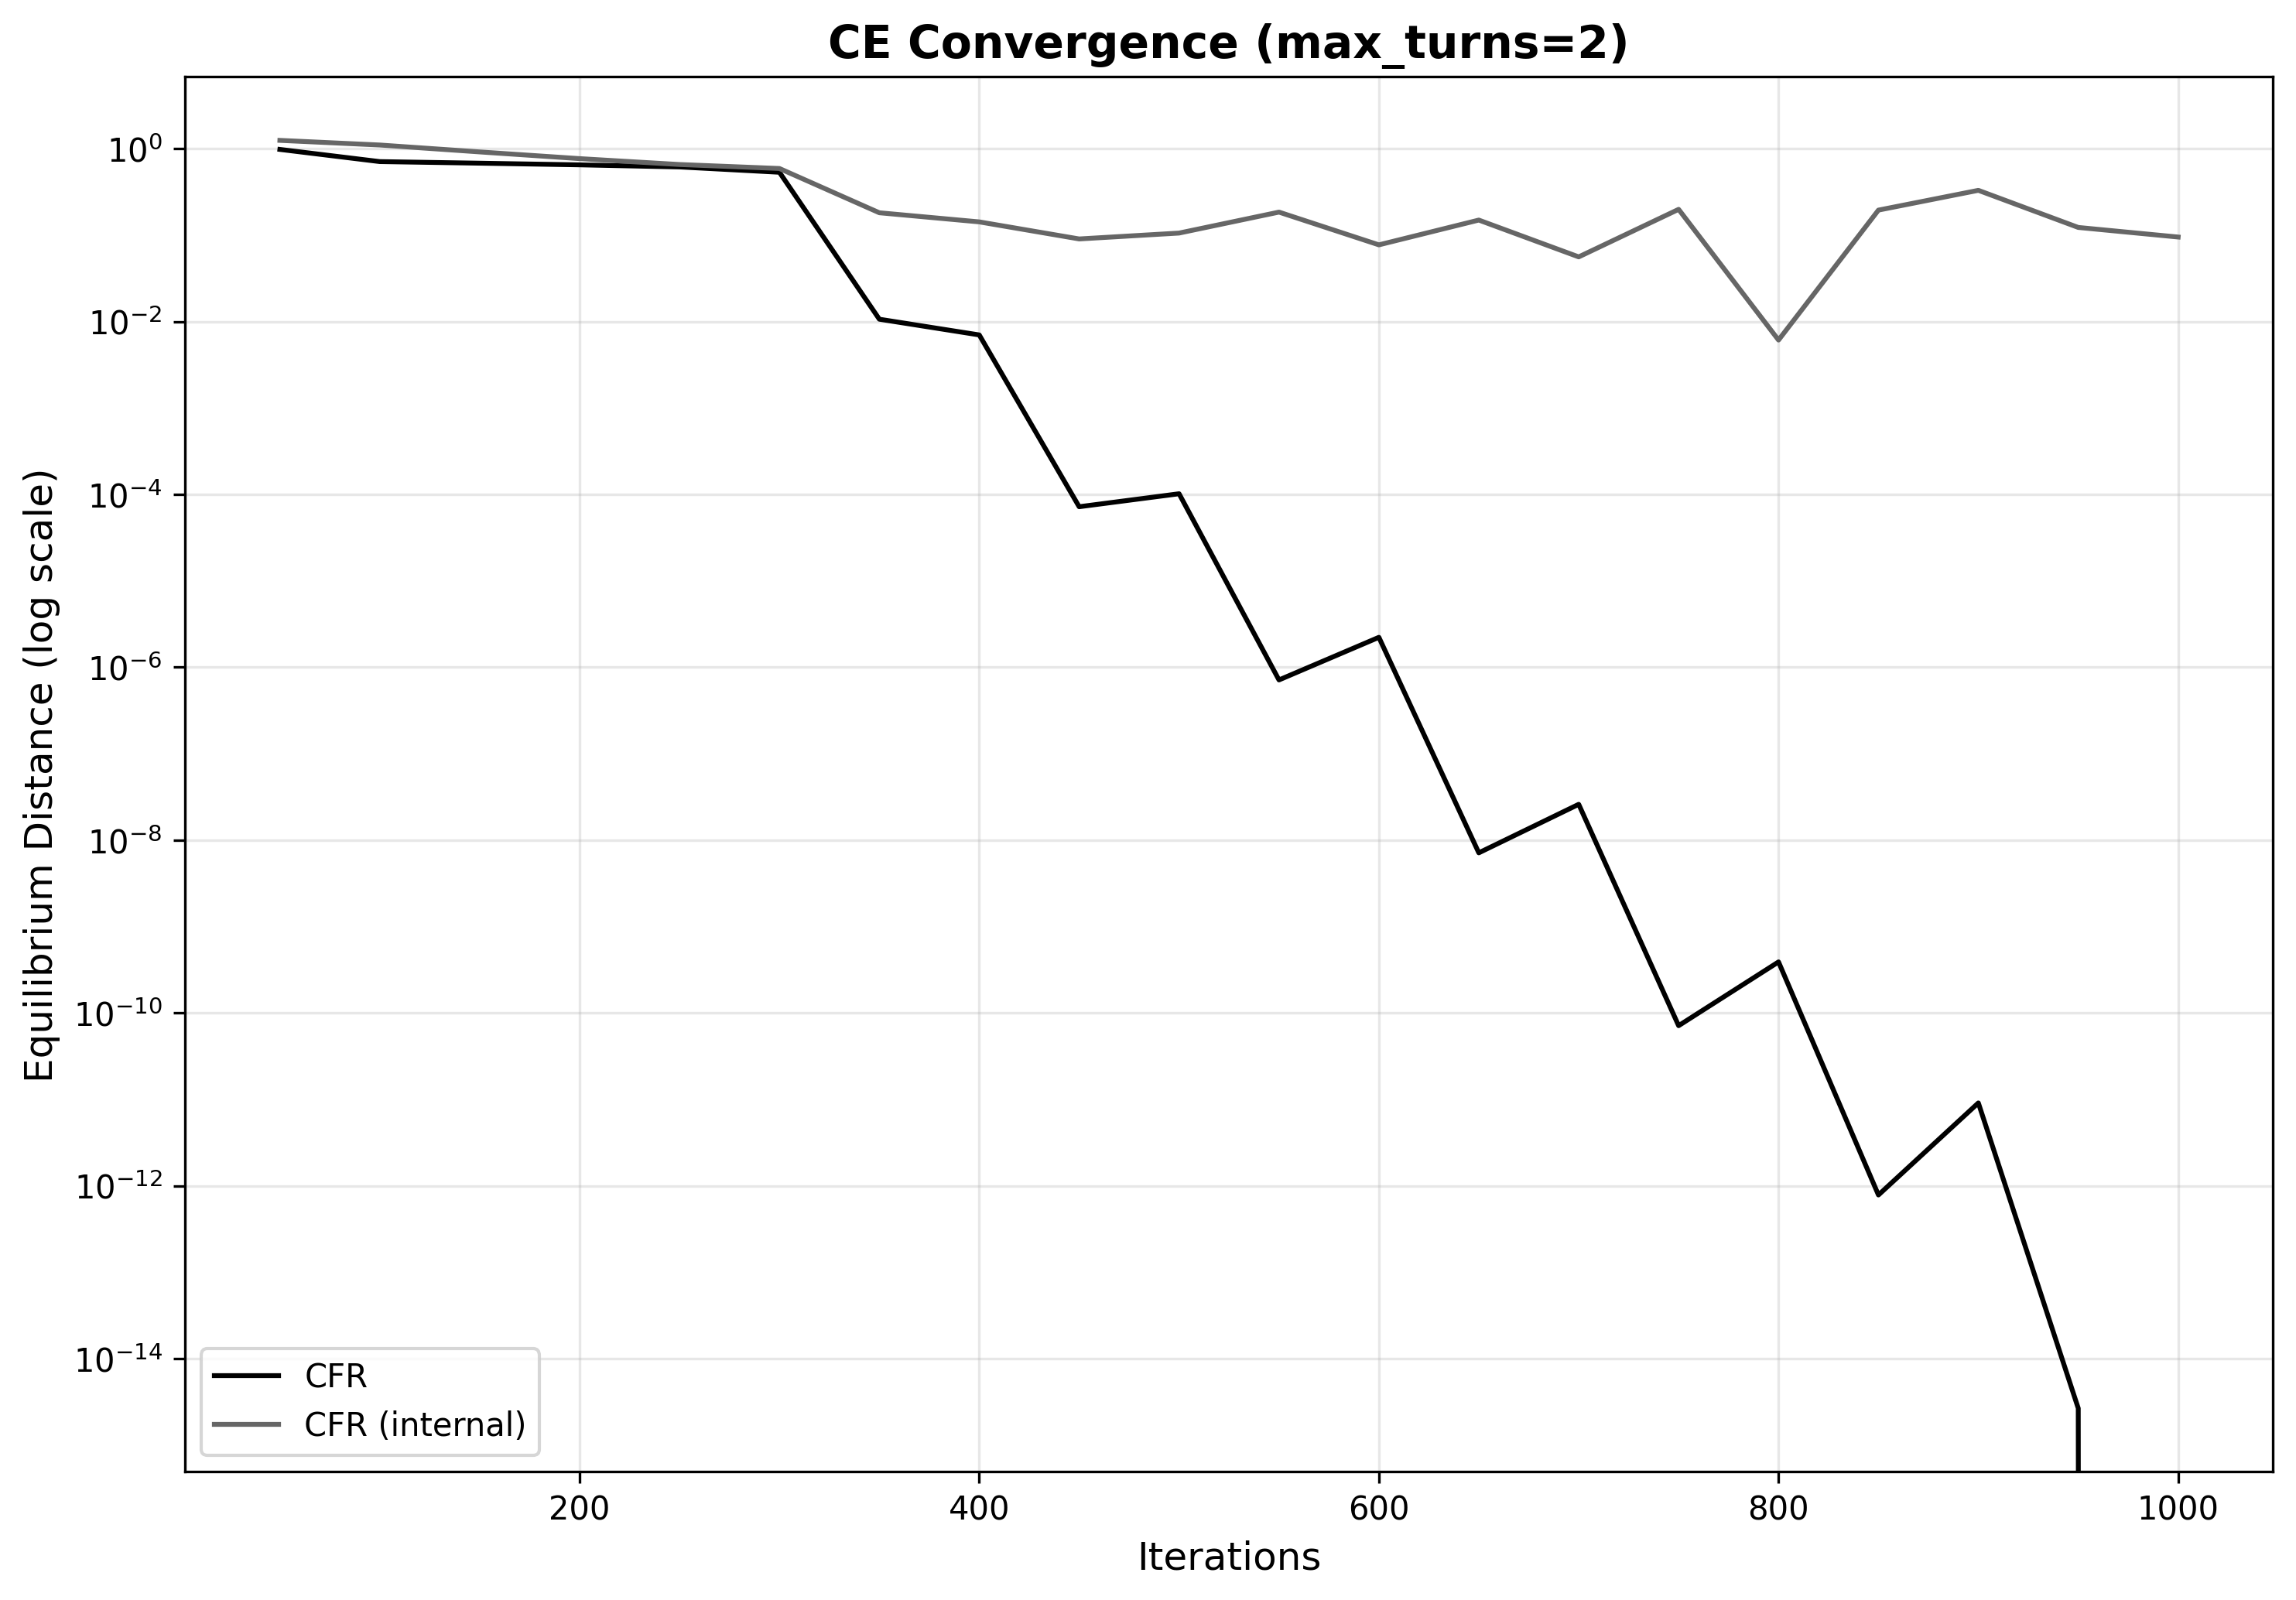
\includegraphics[width=\linewidth]{plots/eq_dist/t2_ce_convergence.png}
  \caption{CE}
\end{subfigure}
\caption{Convergence to each equilibrium concept on \texttt{max\_turns}$=2$, log-scale $y$-axis. Single-seed curves shown directly.}
\label{fig:t2_curves}
\end{figure}

Reading the table column by column:
\begin{itemize}
    \item \textbf{AFCCE.} Both CFR and EFR\_ACT essentially nail zero; the hypothesis (EFR\_ACT minimum) holds, with the qualification that CFR also reaches the floor on this small game.
    \item \textbf{AFCE.} EFR\_ACT\_in (1e-14) versus CFR\_in (0.065): EFR\_ACT\_in beats CFR\_in by 13 orders of magnitude. Hypothesis~2 confirmed cleanly.
    \item \textbf{EFCCE.} \emph{The hierarchy goes the wrong way.} CFR (5e-15) $\approx$ EFR\_CSPS (2e-14) $\prec$ EFR\_TIPS (0.010) $\prec$ EFR\_BHV (0.038). Stronger deviation sets give \emph{larger} EFCCE distance, the opposite of Hypothesis~3. We discuss this in \S\ref{sec:eqdist_disc}.
    \item \textbf{EFCE.} EFR\_BHV\_in (9e-12) $\prec$ EFR\_CFPS\_in (1e-5) $\prec$ EFR\_TIPS\_in (0.032) $\prec$ CFR\_in (0.131). The strongest variant dominates, consistent with Hypothesis~4.
    \item \textbf{CCE.} CFR\_in (5e-08) is far better than CFR (0.013); the converse on CE.
    \item \textbf{CE.} CFR (0) beats CFR\_in (0.095). The pattern in CCE and CE flips, consistent with the coarse/correlated split inherited from external/internal regret.
\end{itemize}

\subsection{Results: 3-Turn Variant}
\label{sec:results_t3}

The 3-turn sweep was run at 100 iterations with random seed 2 (a smaller iteration budget than the 2-turn sweep is sufficient at this depth to make the deviation hierarchy visible before within-run variance dominates the snapshot). Table~\ref{tab:t3_results} reports the final-iteration distance for each (algorithm, equilibrium) cell; Figure~\ref{fig:t3_curves} plots convergence curves.

\begin{table}[H]
\centering
\caption{Final-iteration equilibrium distance on \texttt{max\_turns}$=3$ after 100 iterations, \texttt{random\_seed=2}.}
\label{tab:t3_results}
\begin{tabular}{lcccccc}
\toprule
Algorithm & AFCCE & AFCE & EFCCE & EFCE & CCE & CE \\
\midrule
CFR             & 0.774 &       & 1.289 &       & 1.083 & 1.310 \\
CFR\_in         &       & 0.586 &       & 1.020 & 1.164 & 1.348 \\
EFR\_ACT        & 0.798 &       &       &       &       & \\
EFR\_ACT\_in    &       & 0.587 &       &       &       & \\
EFR\_CSPS       &       &       & 1.155 &       &       & \\
EFR\_TIPS       &       &       & 1.000 &       &       & \\
EFR\_BHV        &       &       & 0.818 &       &       & \\
EFR\_CFPS\_in   &       &       &       & 0.835 &       & \\
EFR\_TIPS\_in   &       &       &       & 0.767 &       & \\
EFR\_BHV\_in    &       &       &       & 0.704 &       & \\
\bottomrule
\end{tabular}
\end{table}

\begin{figure}[H]
\centering
\begin{subfigure}{0.32\textwidth}
  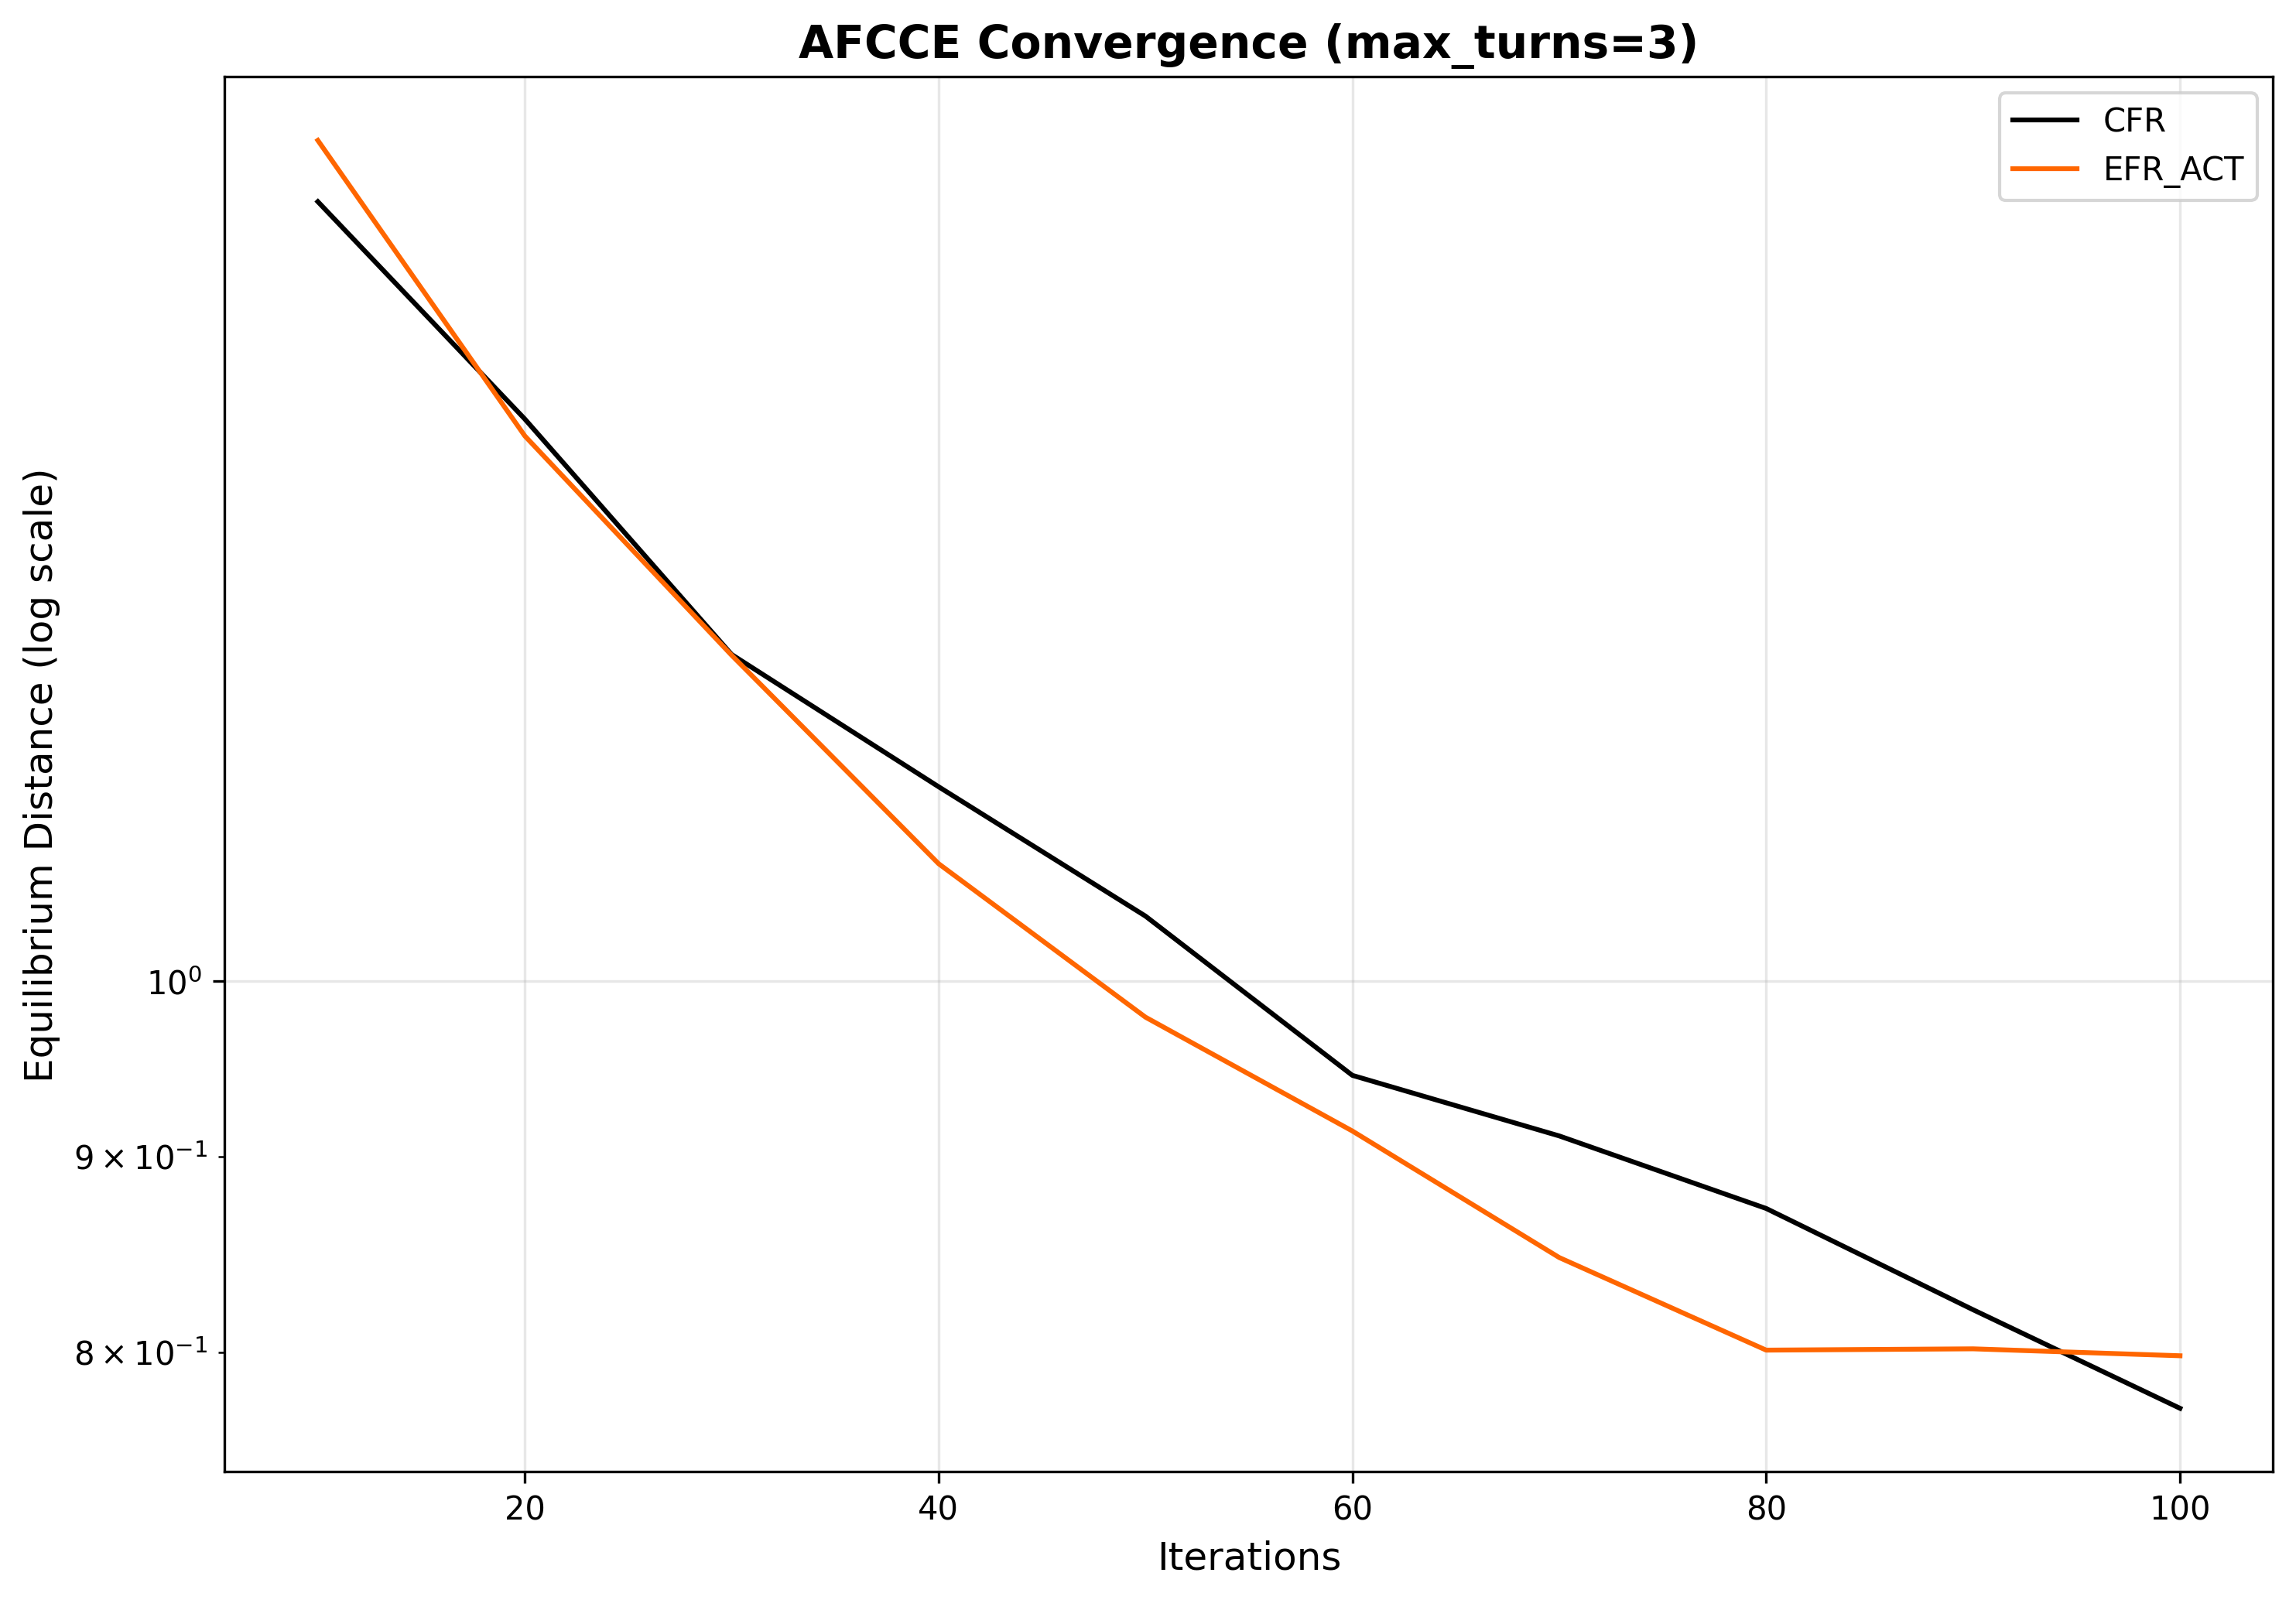
\includegraphics[width=\linewidth]{plots/eq_dist/t3_afcce_convergence.png}
  \caption{AFCCE}
\end{subfigure}
\begin{subfigure}{0.32\textwidth}
  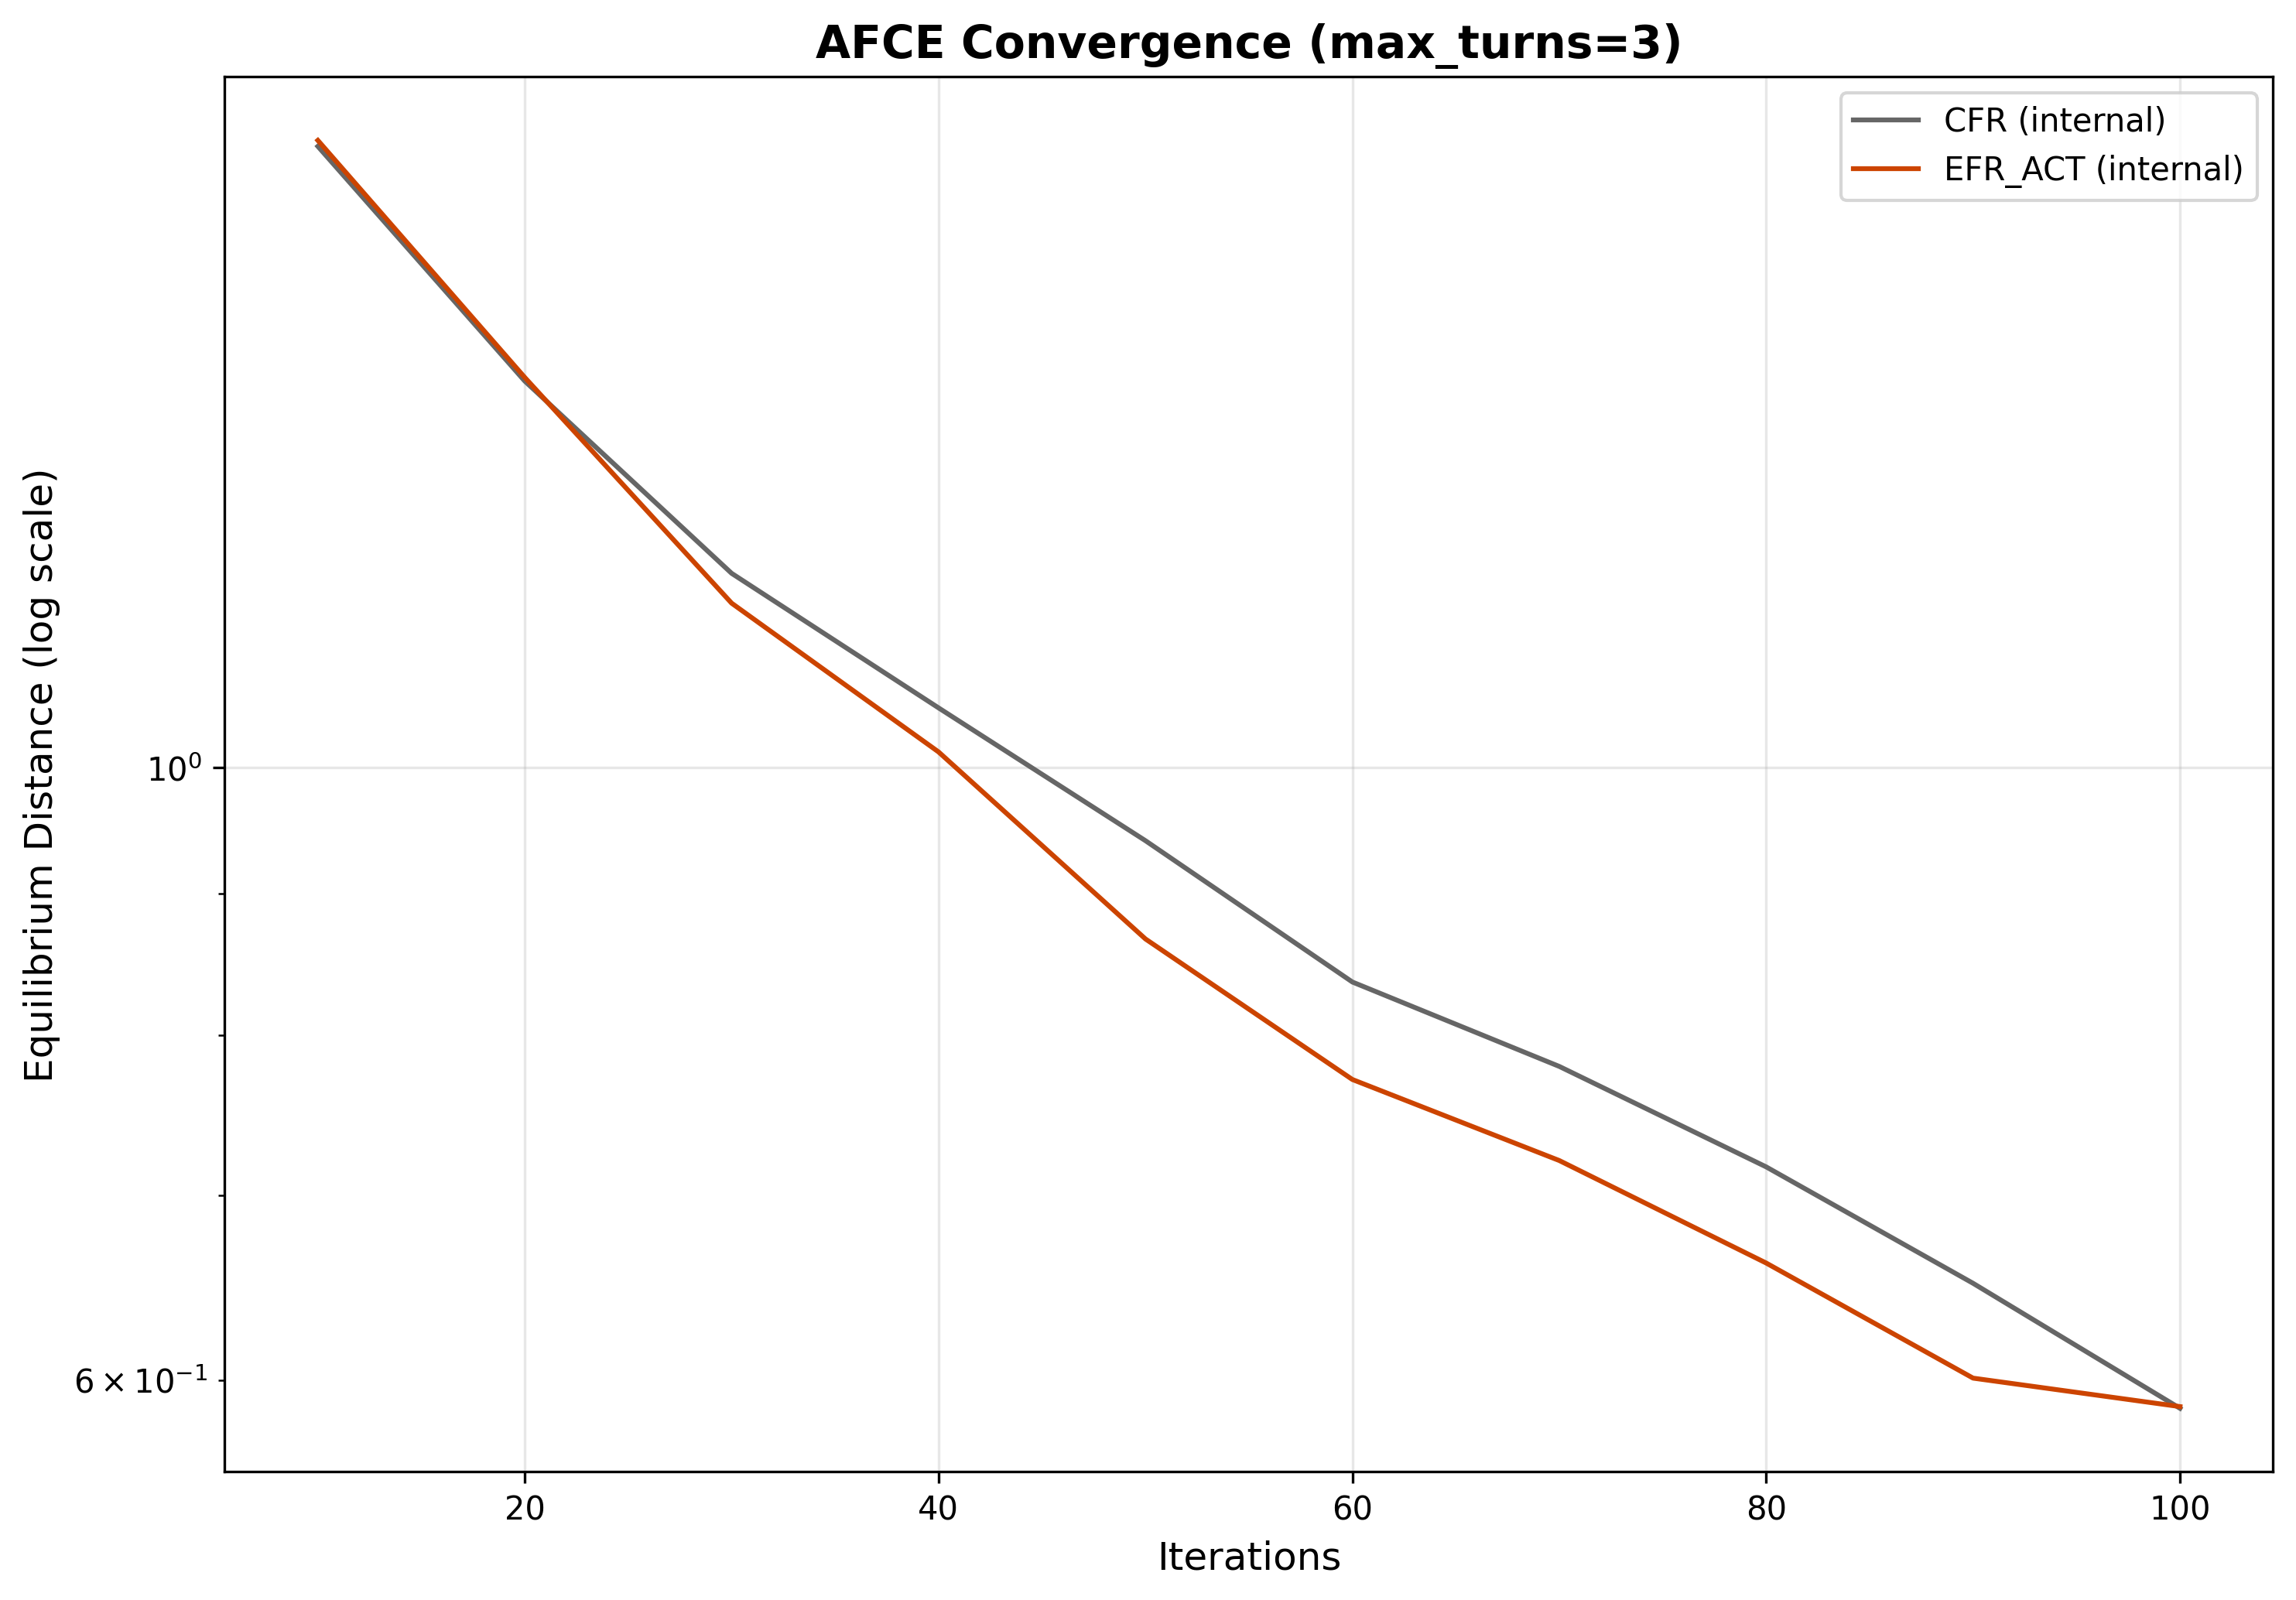
\includegraphics[width=\linewidth]{plots/eq_dist/t3_afce_convergence.png}
  \caption{AFCE}
\end{subfigure}
\begin{subfigure}{0.32\textwidth}
  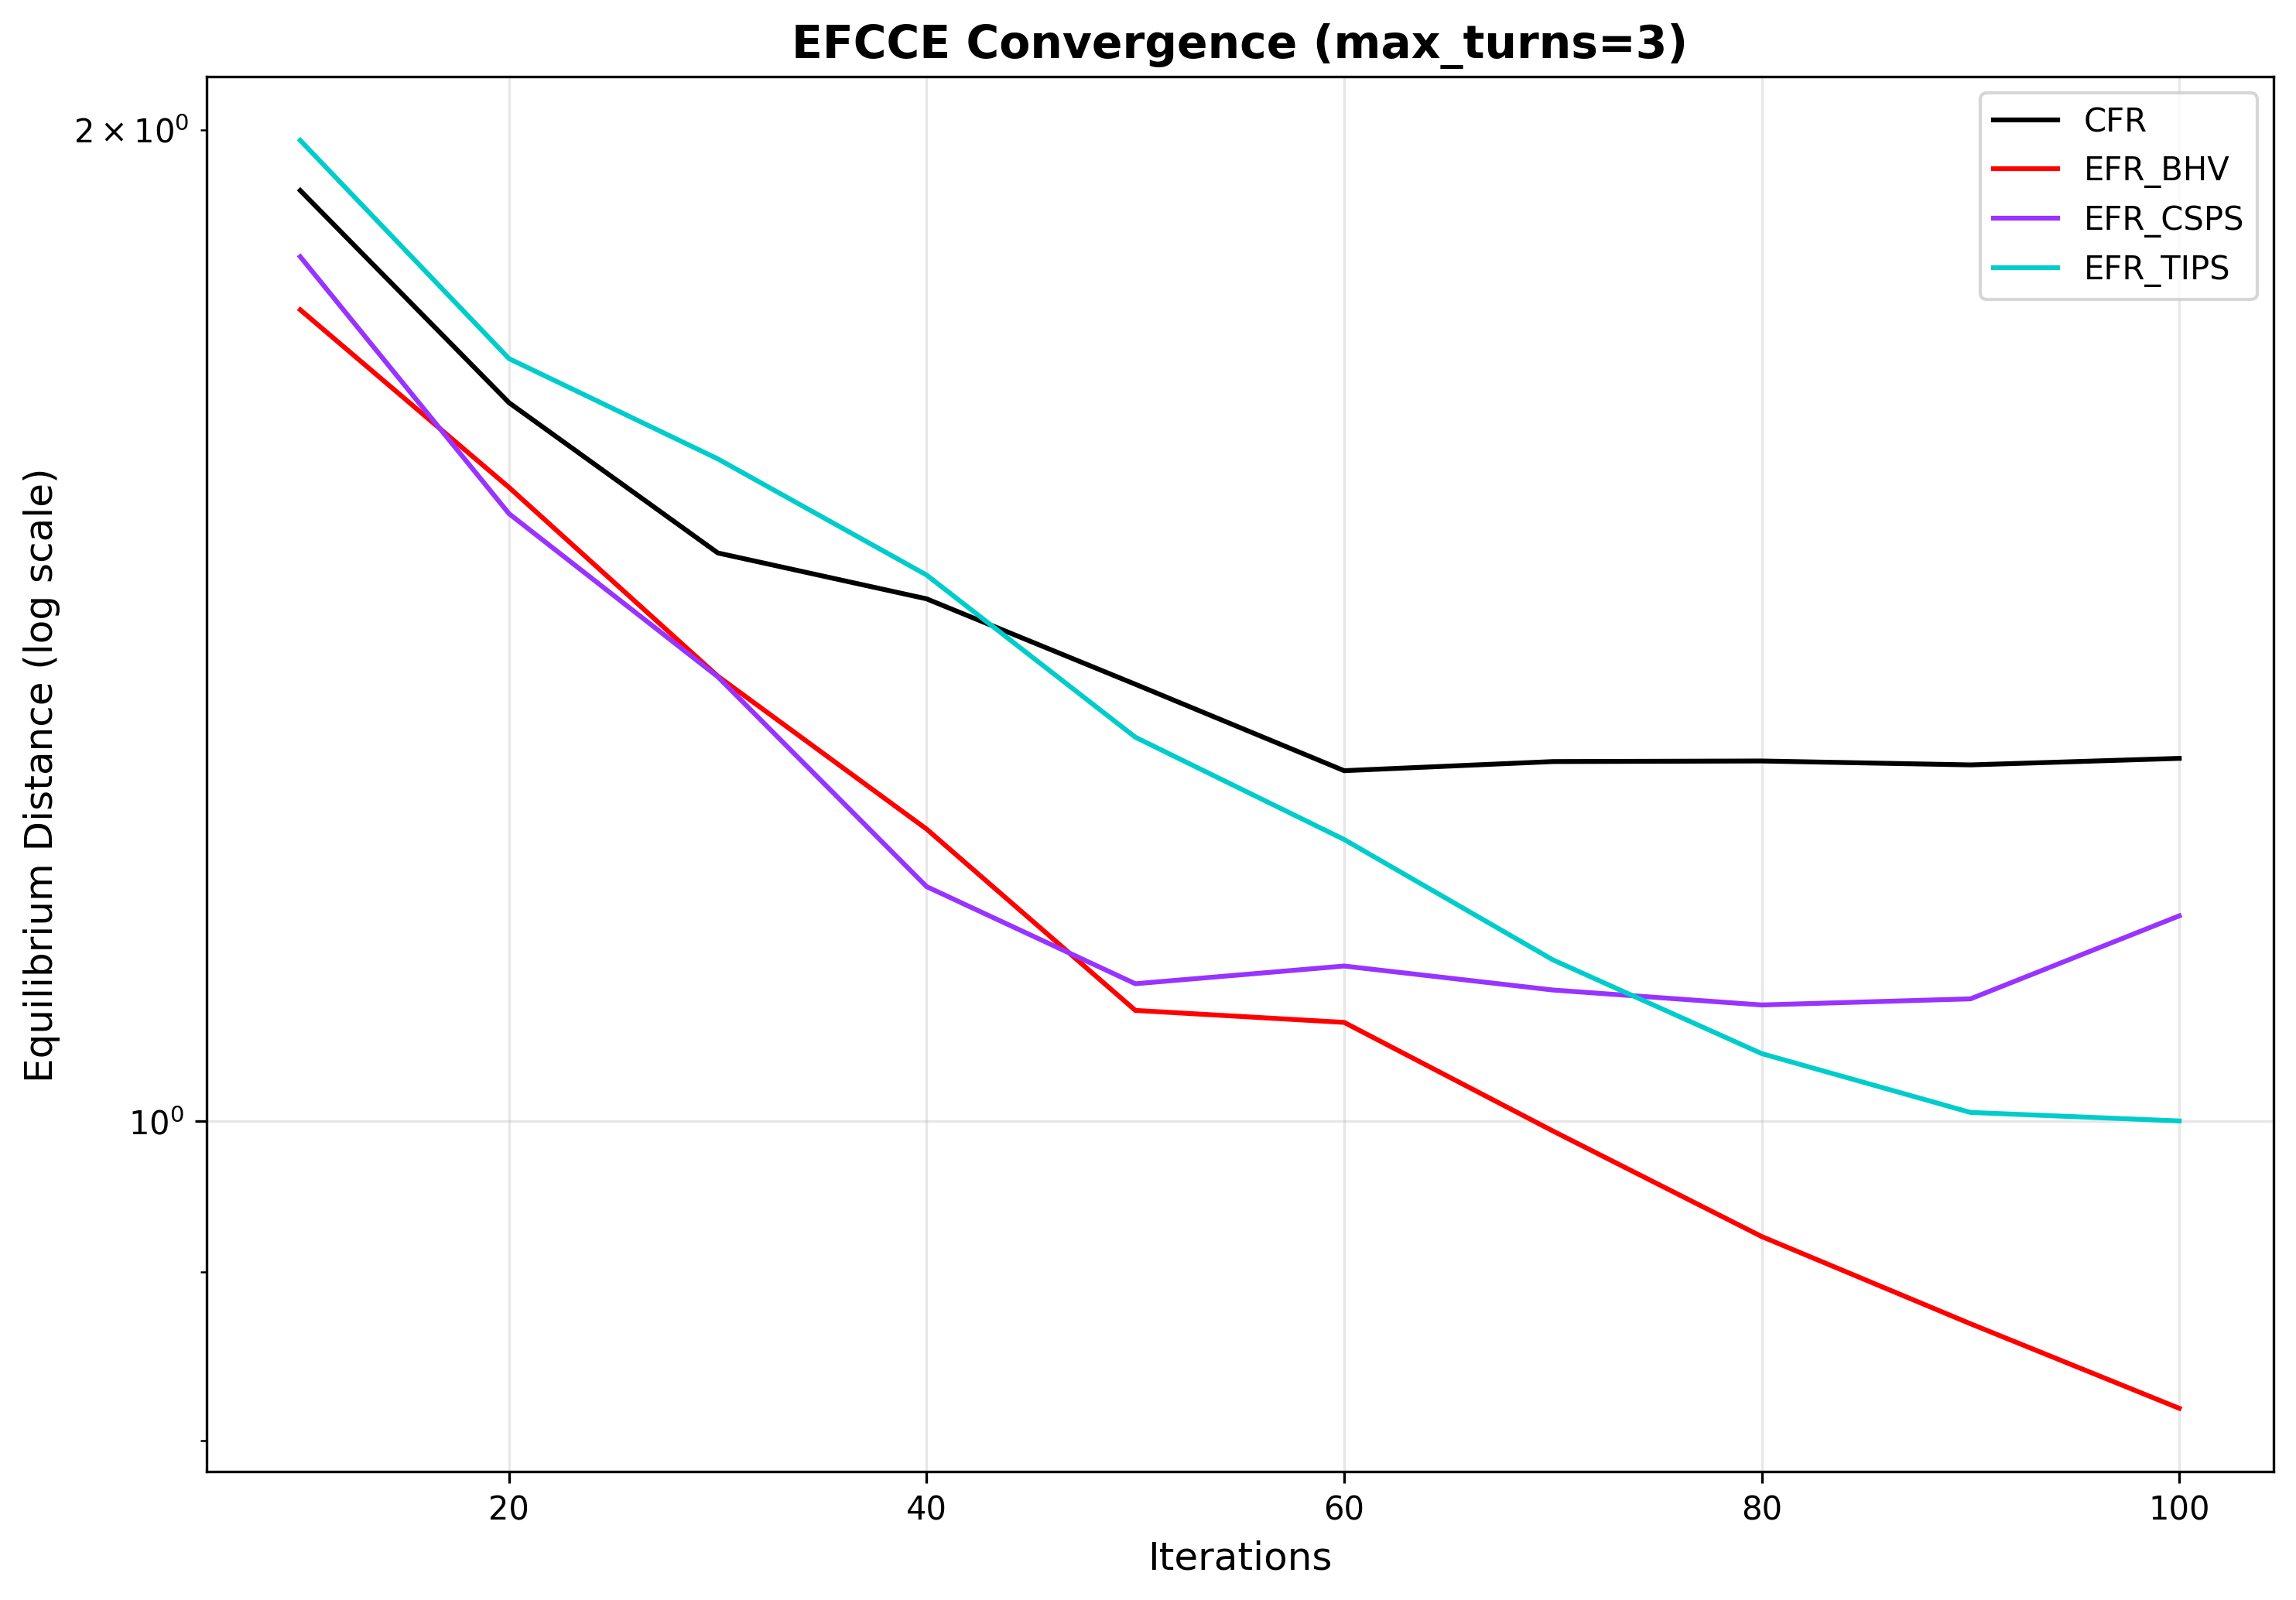
\includegraphics[width=\linewidth]{plots/eq_dist/t3_efcce_convergence.png}
  \caption{EFCCE}
\end{subfigure}

\begin{subfigure}{0.32\textwidth}
  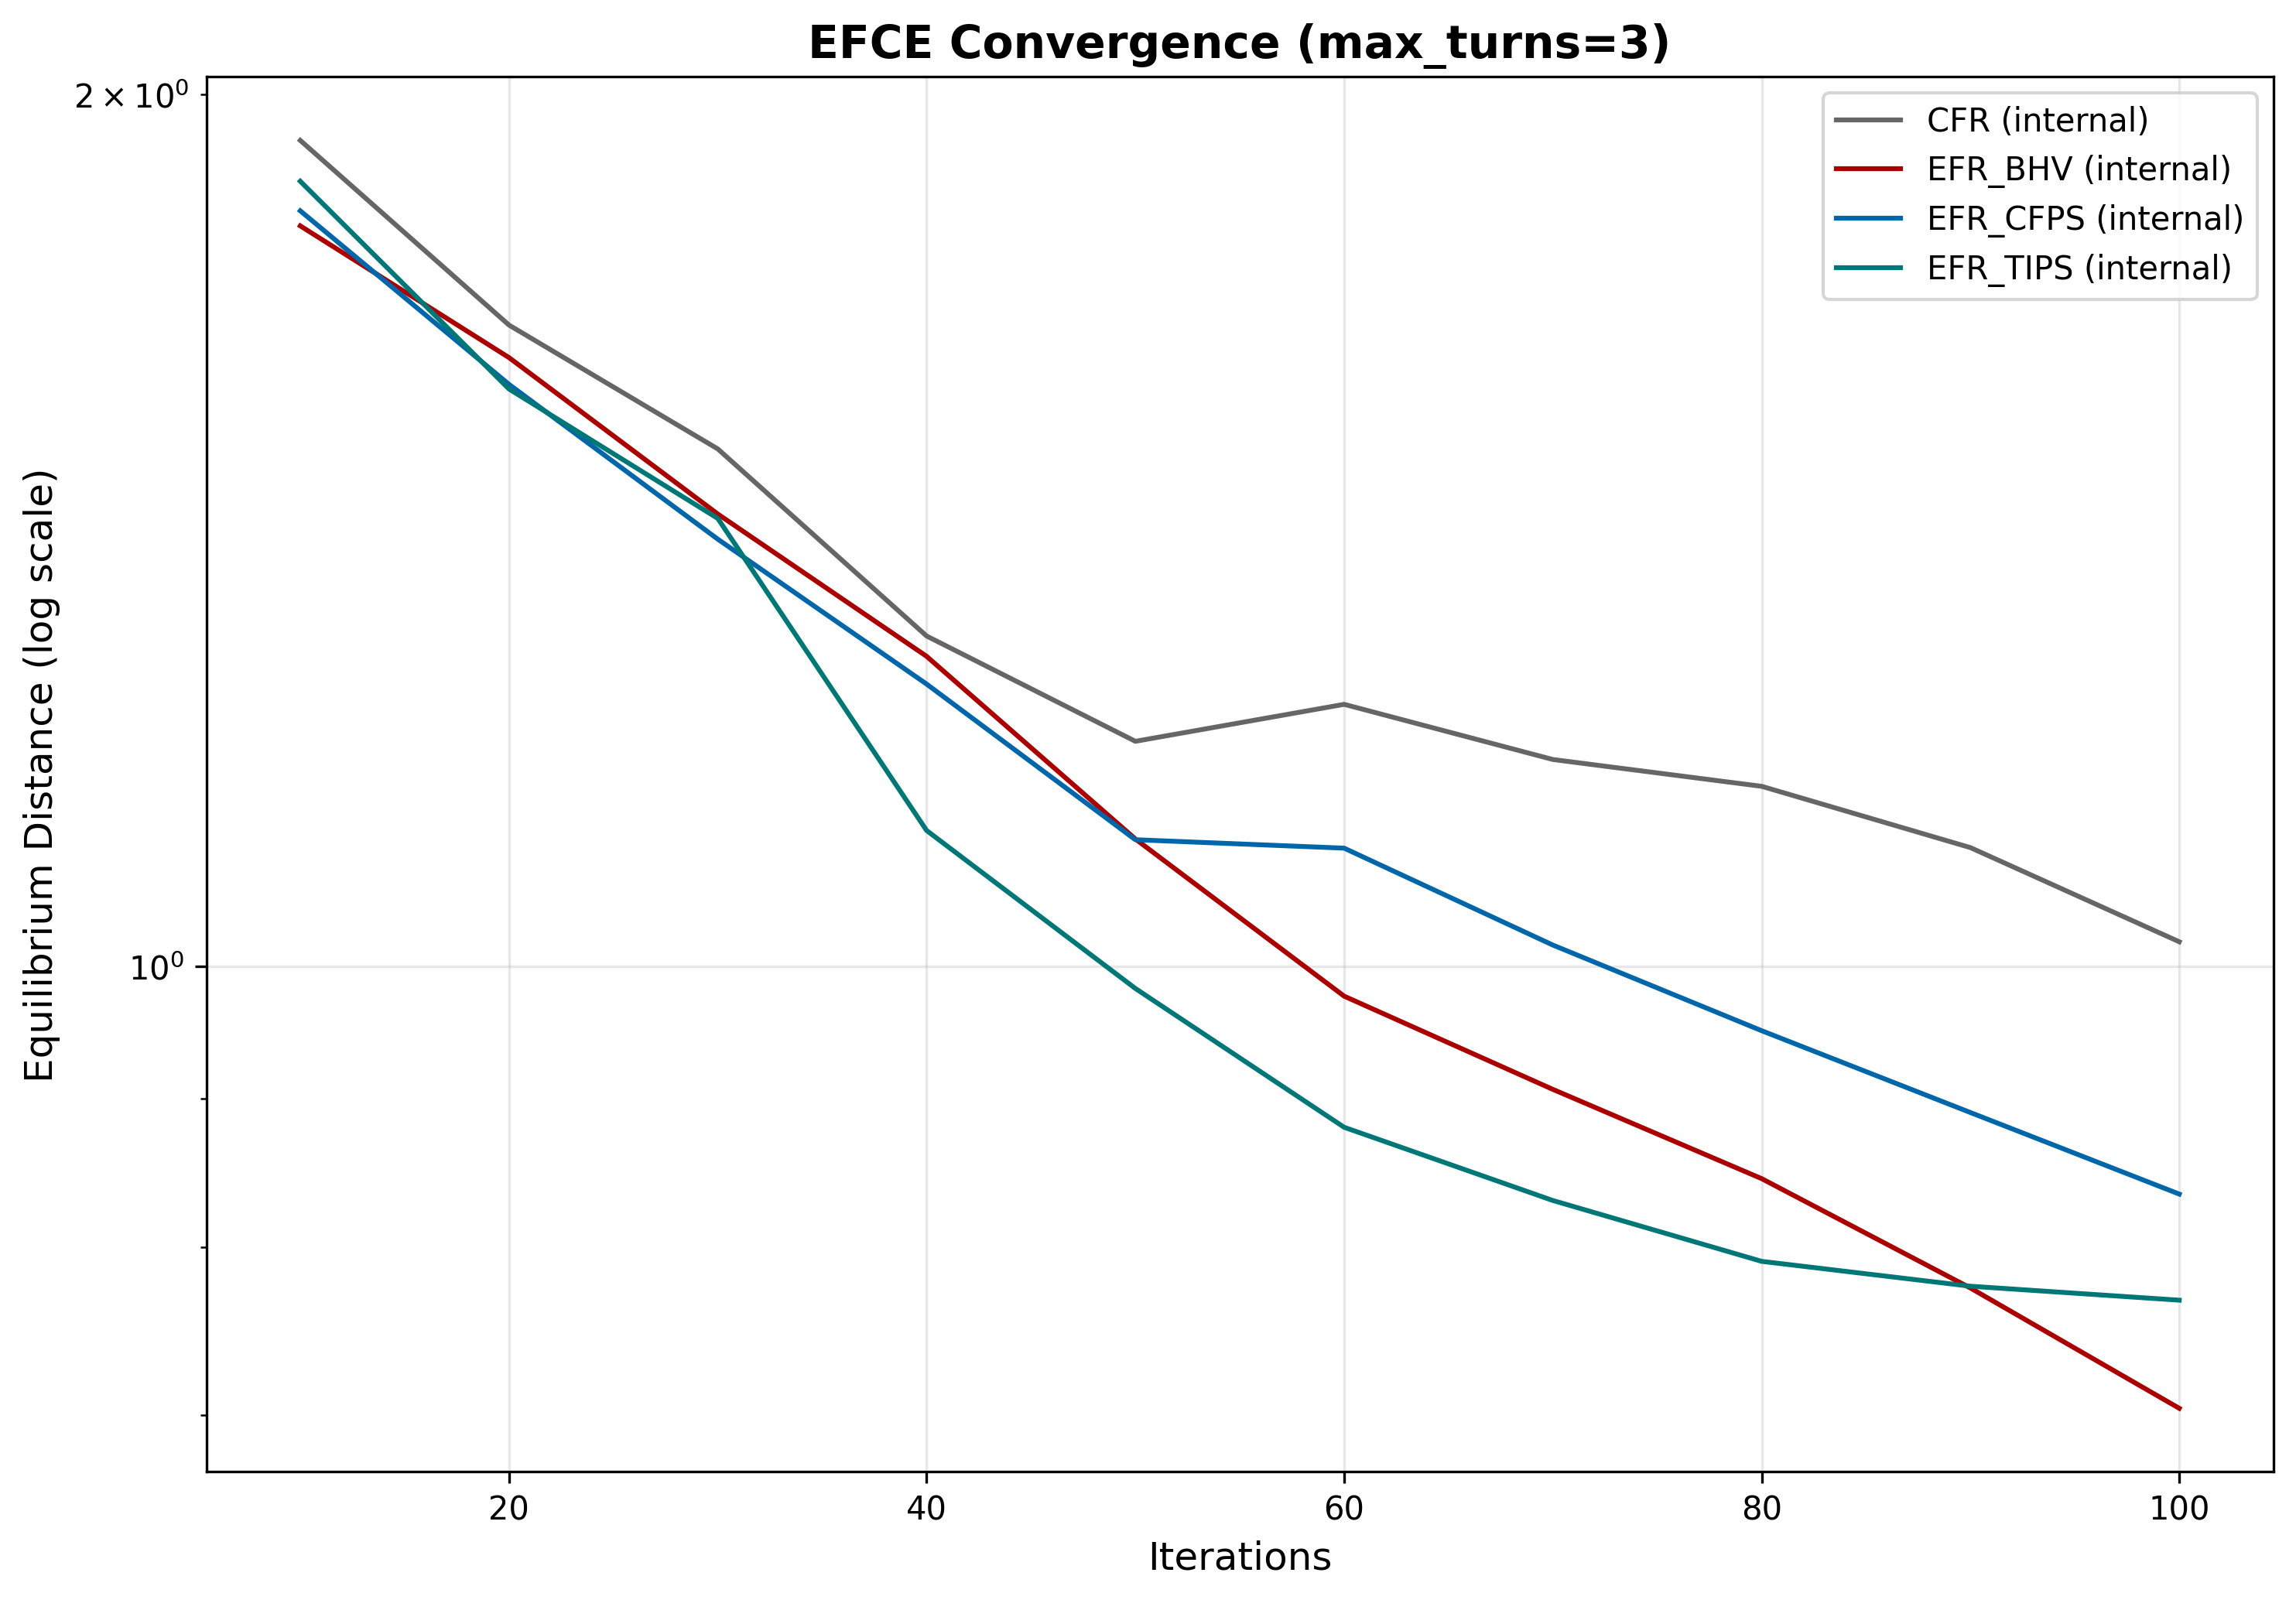
\includegraphics[width=\linewidth]{plots/eq_dist/t3_efce_convergence.png}
  \caption{EFCE}
\end{subfigure}
\begin{subfigure}{0.32\textwidth}
  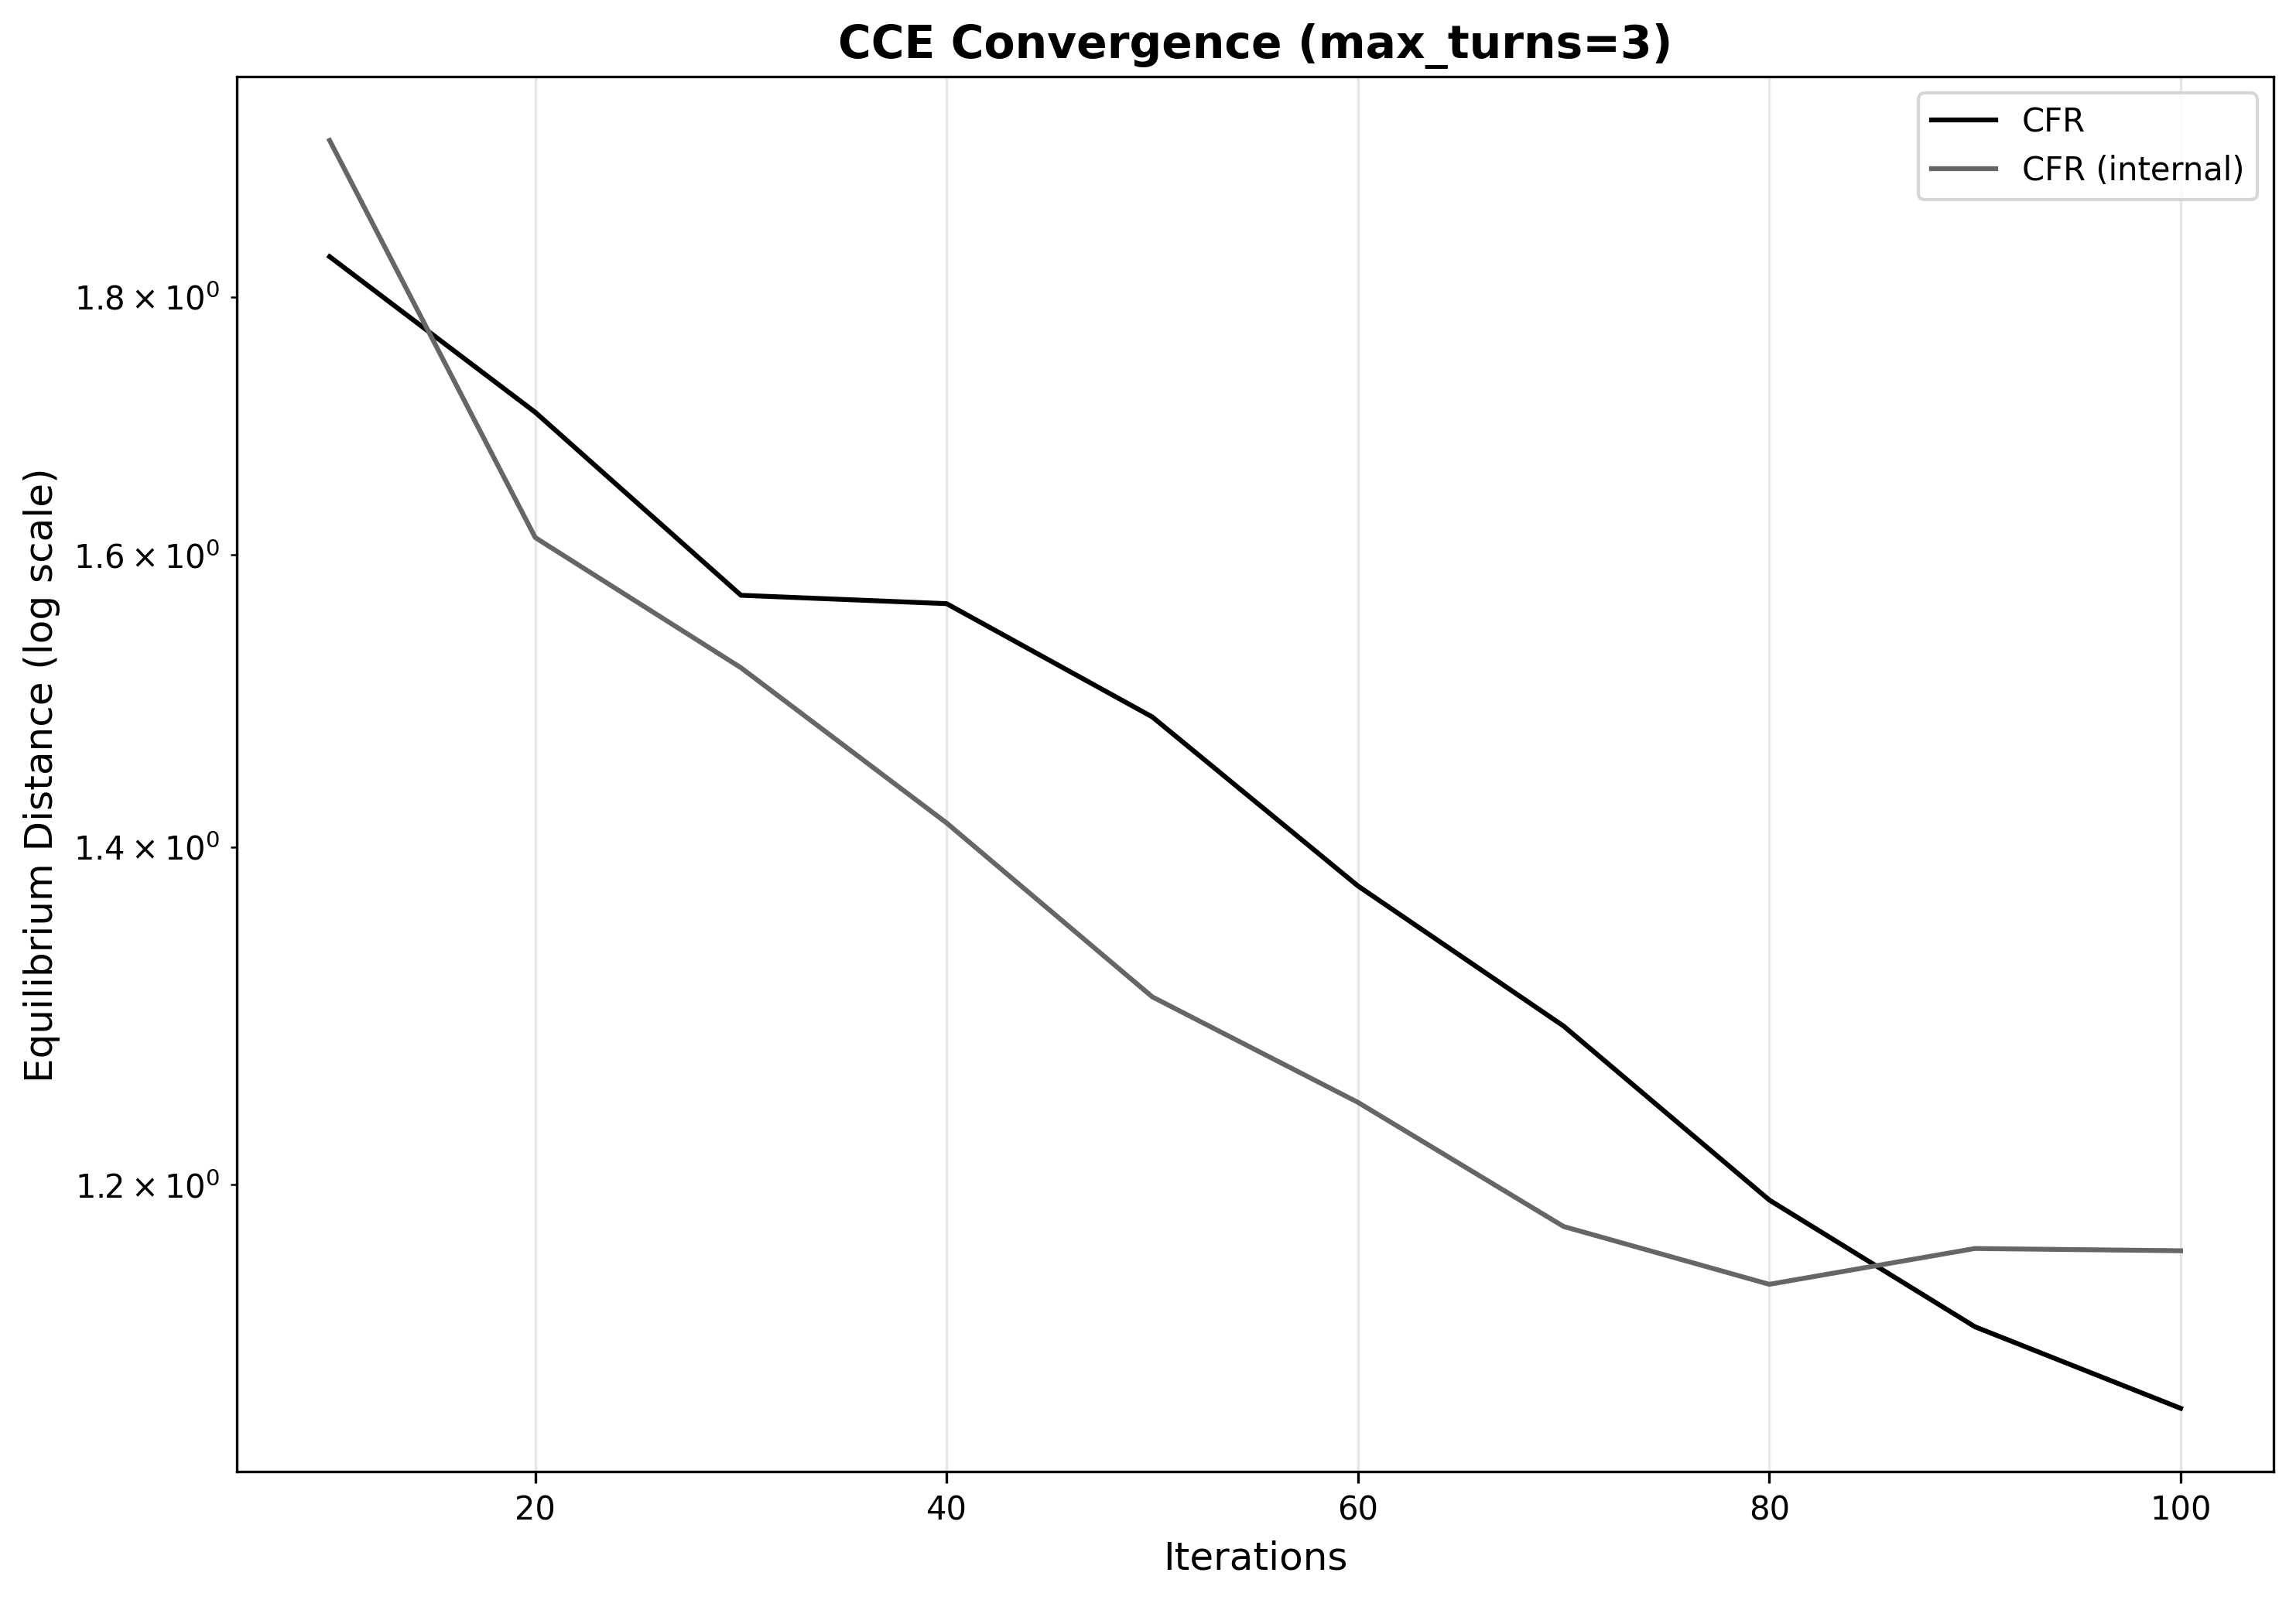
\includegraphics[width=\linewidth]{plots/eq_dist/t3_cce_convergence.png}
  \caption{CCE}
\end{subfigure}
\begin{subfigure}{0.32\textwidth}
  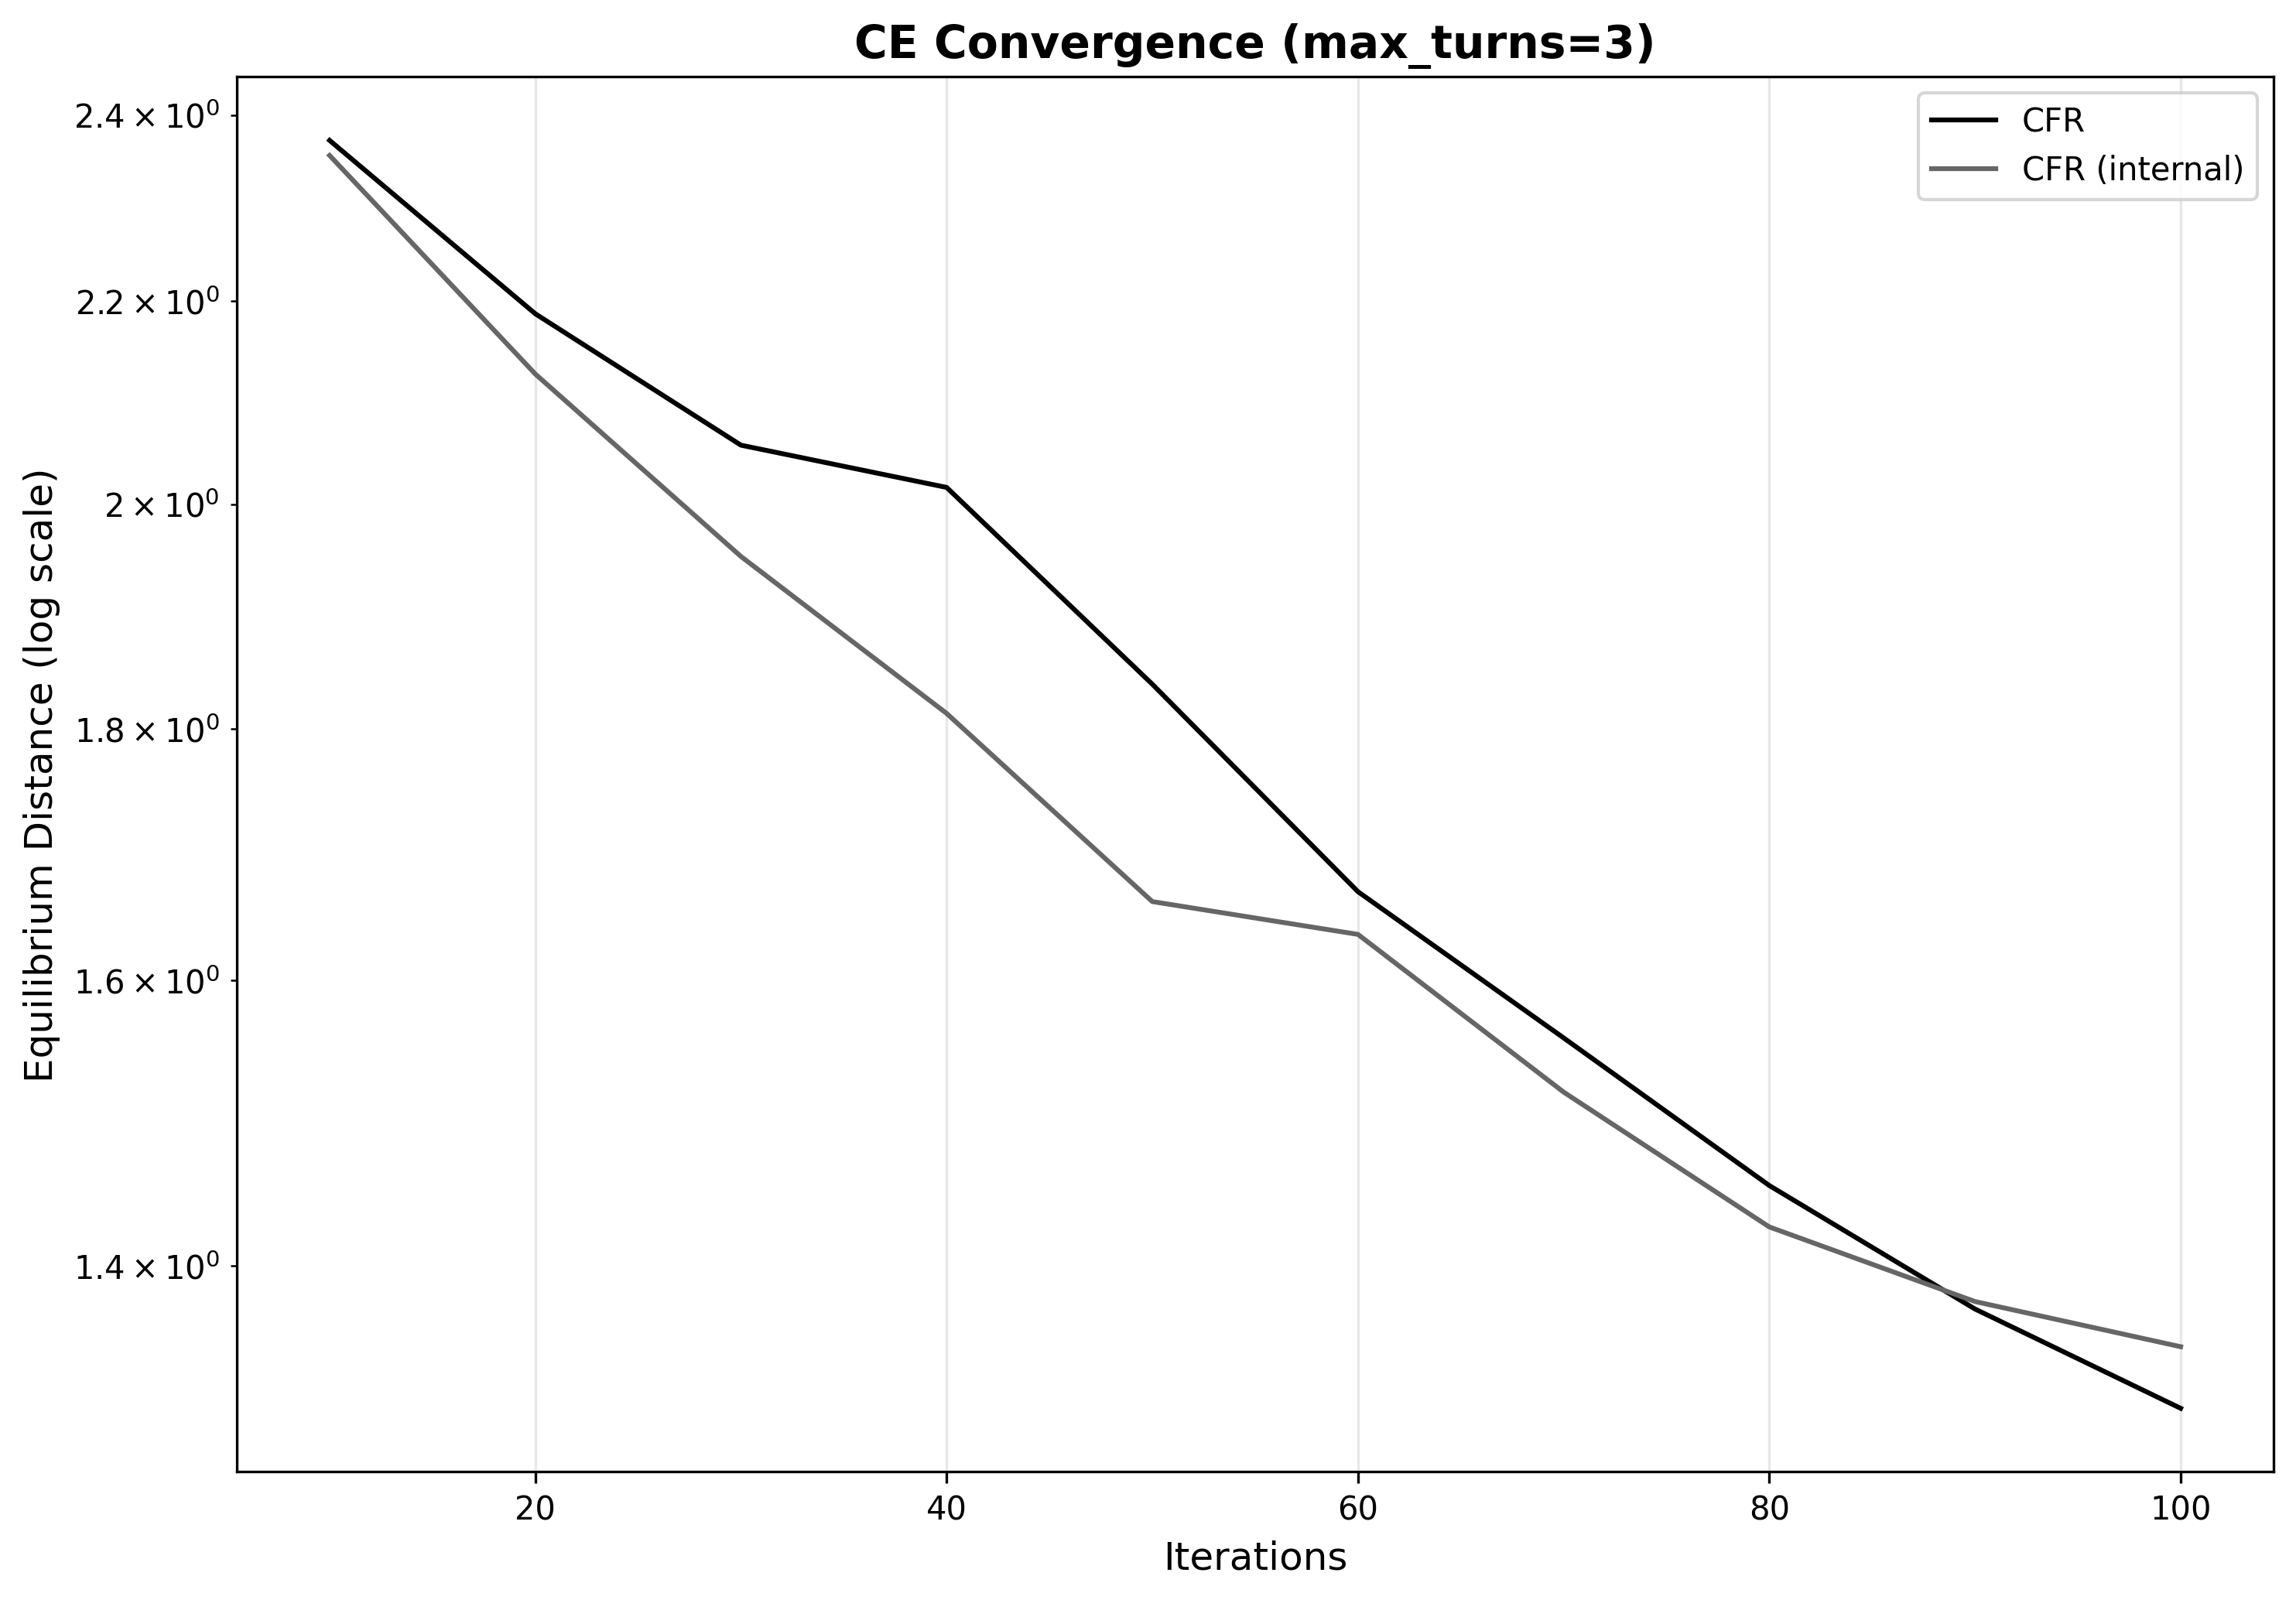
\includegraphics[width=\linewidth]{plots/eq_dist/t3_ce_convergence.png}
  \caption{CE}
\end{subfigure}
\caption{Convergence to each equilibrium concept on \texttt{max\_turns}$=3$, log-scale $y$-axis.}
\label{fig:t3_curves}
\end{figure}

Reading the table column by column:
\begin{itemize}
    \item \textbf{AFCCE.} CFR (0.774) and EFR\_ACT (0.798) are within 3\% of each other, with CFR slightly ahead. The Hypothesis~2 gap (EFR\_ACT $\prec$ CFR on AFCCE) is not visible at this iteration count; both algorithms are still far from convergence on the 3-turn variant.
    \item \textbf{AFCE.} CFR\_in (0.586) and EFR\_ACT\_in (0.587) are essentially tied (within 0.1\%). Same observation as AFCCE.
    \item \textbf{EFCCE.} \emph{Clean strict hierarchy:} CFR (1.289) $\succ$ EFR\_CSPS (1.155) $\succ$ EFR\_TIPS (1.000) $\succ$ EFR\_BHV (0.818). Stronger deviation sets give strictly smaller distances, exactly the ordering predicted by Hypothesis~4 (BHV $\succ$ TIPS $\succ$ CSPS $\succ$ CFR). CFR's distance is roughly $1.58\times$ that of BHV; the spread across the four algorithms is large enough to make the hierarchy unambiguous.
    \item \textbf{EFCE.} \emph{Clean strict hierarchy:} CFR\_in (1.020) $\succ$ EFR\_CFPS\_in (0.835) $\succ$ EFR\_TIPS\_in (0.767) $\succ$ EFR\_BHV\_in (0.704). The full predicted ordering of Hypothesis~5 (BHV$_\text{in}$ $\succ$ TIPS$_\text{in}$ $\succ$ CFPS$_\text{in}$ $\succ$ CFR$_\text{in}$) holds.
    \item \textbf{CCE.} CFR (1.083) $\prec$ CFR\_in (1.164): the external-regret variant produces a profile closer to the normal-form coarse correlated equilibrium than the internal-regret variant. Within 8\% of each other.
    \item \textbf{CE.} CFR (1.310) $\prec$ CFR\_in (1.348): both algorithms remain far from CE at this iteration count, with CFR slightly ahead.
\end{itemize}

\subsection{Results: 4-Turn Variant}

The 4-turn sweep is queued but has not started at time of writing.\footnote{Runtime estimate: with each 4-turn run taking 10 to 25 minutes and 16 runs sequentially, the 4-turn sweep alone takes roughly four hours of wall-clock time.} Tables and figures for this variant will mirror the structure of \S\ref{sec:results_t2}.

\subsection{Discussion}
\label{sec:eqdist_disc}

\paragraph{The deviation hierarchy holds.} The 3-turn data confirms the central prediction of Morrill et al.~(2021b) on \emph{Deal or No Deal}: stronger deviation sets give strictly smaller equilibrium distances under the matching equilibrium concept. On EFCCE, the ordering CFR $\succ$ EFR\_CSPS $\succ$ EFR\_TIPS $\succ$ EFR\_BHV (Hypothesis~4) holds exactly, with CFR's distance roughly $1.58\times$ that of BHV. On EFCE the full ordering CFR$_\text{in}$ $\succ$ EFR\_CFPS$_\text{in}$ $\succ$ EFR\_TIPS$_\text{in}$ $\succ$ EFR\_BHV$_\text{in}$ (Hypothesis~5) holds without any swaps; CFR$_\text{in}$'s distance is $1.45\times$ BHV$_\text{in}$'s. Both concepts therefore confirm the strict deviation-strength ordering predicted by Morrill et al.\ on this domain.

\paragraph{Game-length scaling.} The 2-turn variant is small enough that several matched algorithms reach machine-precision distance on the matched concept (e.g.\ EFR\_ACT on AFCCE, EFR\_ACT\_in on AFCE, EFR\_BHV\_in on EFCE), making the hierarchy invisible because the floor compresses everything. The 3-turn variant is exactly the regime where the hierarchy is most legible: distances are non-trivial across all algorithms, and the deviation-strength ordering shows up cleanly in the relative spreads. The 4-turn data, when complete, will determine whether the hierarchy extends to the deepest game tree we examine or whether it begins to break down under added variance from longer paths.

\paragraph{Iteration budget at depth.} The 3-turn results in this section come from a 100-iteration sweep, in contrast to the 1{,}000-iteration 2-turn sweep. We chose this shorter budget after observing that for the most expressive deviation sets (CSPS, TIPS, BHV), the per-iteration distance estimate is dominated by oscillation in the empirical correlation device at later iterations: the average policy is still descending in mean but the snapshot at any single iteration jumps within a wide range. Earlier in training, before the regret tables for the richer deviation sets accumulate enough variance to drive these oscillations, the deviation hierarchy is more cleanly visible because all algorithms are descending monotonically from the uniform-strategy starting point. The 100-iteration budget is short enough to sit before this oscillation regime and long enough for the algorithms to differentiate.

\paragraph{Two anomalies on the matched-action concepts.} On AFCCE at 3 turns, CFR (0.774) and EFR\_ACT (0.798) are within 3\% of each other, with CFR slightly ahead. On AFCE, CFR\_in (0.586) and EFR\_ACT\_in (0.587) are essentially tied. The Hypothesis~2 / Hypothesis~3 prediction (action-deviation EFR variants strictly beat CFR / CFR\_in on these concepts) is not visible at this depth and iteration count. We attribute this to a regret-table-size effect: at 100 iterations, the action-deviation EFR variants have not yet differentiated their cumulative regret tables enough to pull ahead of plain counterfactual regret on the relatively coarse AFCCE / AFCE concepts. The same algorithms reach machine-precision distance on these concepts at 2 turns (where iter budget is 1{,}000) and would presumably pull ahead at 3 turns given more iterations. The pattern on EFCCE / EFCE, where the hierarchy holds clearly at 100 iterations, indicates that the deviation-class distinction matters more for the sequential equilibrium concepts than for the agent-form ones at this iteration budget.

\newpage

\part{Monte Carlo Extensive-Form Regret Minimization}

This part of the thesis answers Sub-question~2. Part~I established the qualitative behavior of EFR variants on a tractable benchmark; here we turn to the algorithmic question that determines whether EFR can be applied beyond such benchmarks. We develop a Monte Carlo extension of EFR (MC-EFR) that lifts the exact-update requirement, supporting external-sampling and outcome-sampling traversals across all standard deviation types. \S\ref{sec:mcefr_gap} establishes the gap; \S\ref{sec:mcefr_bg} and \S\ref{sec:mcefr_derivation} develop the algorithm conceptually; \S\ref{sec:mcefr_ext} states it as Algorithm~\ref{alg:mcefr}; \S\ref{sec:mcefr_impl} documents the implementation; \S\ref{sec:mcefr_conv} discusses convergence informally; and \S\ref{sec:mcefr_validation} specifies validation experiments against exact EFR on the Part~I benchmark. This is the central algorithmic contribution of the thesis.

\section{The Gap}
\label{sec:mcefr_gap}

Morrill et al.~(2021b), in the Discussion subsection of EFR (\S6.4 of the corrected version), make a single passing claim about Monte Carlo extensions:
\begin{quote}
``EFR inherits CFR's flexibility as it can be used with Monte Carlo sampling [Lanctot et al.\ 2009; Burch et al.\ 2012; Gibson et al.\ 2012; Johanson et al.\ 2012], function approximation\ldots, variance reduction\ldots, and predictions\ldots''
\end{quote}
The four citations are all to MC\emph{CFR} papers; none describe a Monte Carlo extension of EFR specifically. The paper's experimental section is explicit on this point (\S7):
\begin{quote}
``Since we evaluate expected payoff, use \emph{expected EFR updates}, and use \emph{exact regret matching}, all results are deterministic and hyperparameter-free.''
\end{quote}
So the EFR paper introduces the algorithm with exact updates only, and claims (without further development) that Monte Carlo sampling could in principle be applied to it. There is no algorithmic specification, no regret bound, no convergence analysis, and no experiment. The OpenSpiel reference implementation released alongside the paper (\texttt{open\_spiel/python/algorithms/efr.py}) is also exact-only. To our knowledge, the present work is the first to specify, implement, and empirically evaluate a Monte Carlo EFR algorithm.

This part closes that gap. We adapt the two most widely used MCCFR sampling schemes (external sampling and outcome sampling; Lanctot et al., 2009) to the EFR setting, addressing the specific complications introduced by EFR's per-deviation memory probabilities. Both variants are implemented in \texttt{dealornodeal/algos/mcefr.py} and benchmarked against exact EFR in \S\ref{sec:mcefr_validation}.

\section{Background: Sampling in Counterfactual Regret Minimization}
\label{sec:mcefr_bg}

Standard CFR (Zinkevich et al., 2007) traverses the full game tree on each iteration to compute the counterfactual regret
\[
\rho^{CF}_I(a;\pi) = v_I(a;\pi) - \mathbb{E}_{a'\sim\pi_i(I)}[v_I(a';\pi)]
\]
at every information set $I$. The cost of one iteration is therefore proportional to the number of information sets times the branching factor.

MCCFR replaces the full traversal with a sampled traversal. Lanctot et al.\ (2009) introduced two schemes that remain the dominant choices in practice:

\paragraph{External sampling (Lanctot et al., 2009, \S4.1).} On the iteration where player $i$ is the \emph{updating} player, the traversal samples actions at every \emph{other} player's nodes (and at chance nodes) according to those players' current strategies, but enumerates all of player $i$'s own actions. Each visited action $a \in A(I)$ at one of player $i$'s information sets receives an unbiased estimate of its counterfactual value $v_I(a;\pi)$, scaled by the inverse of the sampling probability of the path leading to $I$. The estimator is unbiased and zero-variance for the updating player's own choices, so external sampling typically converges nearly as fast as exact CFR per iteration while costing far less.

\paragraph{Outcome sampling (Lanctot et al., 2009, \S4.2).} A single terminal history $z$ is sampled from a sampling distribution $q$ per iteration, and the regrets at every information set on that path are updated using importance-sampled counterfactual values, weighted by the trajectory reach ratio $\pi_{-i}(z)/q(z)$. Outcome sampling is the cheapest per iteration but suffers higher per-iteration variance, and consequently requires more iterations to converge.

Both schemes preserve CFR's central no-regret guarantee (average regret vanishes in expectation) at the cost of variance terms that depend on the sampling distribution.

\section{From MCCFR to MC-EFR}
\label{sec:mcefr_derivation}

EFR's per-iteration update (Algorithm~1 of Morrill et al., 2021b) is structurally similar to CFR's: at each information set $I$ and each \emph{realizable memory state} $g \in G_i(I,\phi)$, accumulate immediate regret weighted by the memory probability $w_\phi(I,g;\pi_i^t)$, then update the strategy via a regret-matching fixed point that aggregates over the deviations $\phi_I \in \Phi_I$ and the time-selection functions $W_I^\Phi(\phi_I)$. This structure suggests three immediate questions when moving to a sampled estimator.

\paragraph{1. What is sampled.} CFR's update needs a counterfactual value $v_I(a;\pi)$ for each $a \in A(I)$. EFR's update needs the same counterfactual value, since the immediate regret of an action transformation $\phi_I$ at memory state $g$ reduces to $w_\phi(I,g;\pi_i)\rho^{CF}_I(\phi_I;\pi)$ where $\rho^{CF}_I(\phi_I;\pi) = \mathbb{E}_{a\sim\phi_I(\pi_i(I))}[\rho^{CF}_I(a;\pi)]$ (Morrill et al., 2021b, \S6.3). So at the level of \emph{what is sampled} in the game tree, MC-EFR is identical to MCCFR: one or more terminal histories drawn from a chosen sampling distribution, importance-weighted to yield unbiased estimates of $v_I(a;\pi)$. The tree-traversal step is therefore unchanged from MCCFR; only the per-information-set update (\S\ref{sec:mcefr_ext}, step~3) is novel.

\paragraph{2. How memory probabilities interact with sampling.} The first non-trivial difference is the memory probability $w_\phi(I,g;\pi_i^t)$. In exact EFR this quantity is computed deterministically from the current strategy by chaining $\pi_i(\cdot \mid I')$ across information sets $I'$ on the path to $I$ (Morrill et al., \S6.2). Under sampling, the path itself is stochastic, but $w_\phi$ remains a function of the (now-sampled) trajectory and the current strategy: it does not introduce a second sampling distribution. We compute $w_\phi$ along the sampled path exactly as in exact EFR; the only difference is which information sets are visited on a given iteration. This is the key property that lets MC-EFR reuse the deviation scaffolding wholesale.

\paragraph{3. How the regret-matching fixed point is preserved.} EFR's regret-matching step at $I$ solves for an immediate strategy $\pi_i^{t+1}(I)$ that is a fixed point of a linear operator built from the per-deviation weights
\[
y_{\phi_I}^{t+1} = \sum_{w \in W_I^\Phi(\phi_I)} w^{t+1}\,\bigl(\rho^{1:t}_{I,w}(\phi_I)\bigr)_+,
\]
following Corollary~1 of Morrill et al.\ (2021b). Sampling affects the cumulative regret table $\rho^{1:t}_{I,w}$ through unbiased estimators, but the fixed-point equation $\pi_i^{t+1}(I) = (1/z^{t+1}) \sum_{\phi_I} y^{t+1}_{\phi_I} \phi_I(\pi_i^{t+1}(I))$ at the moment of strategy reconstruction is unchanged.

These three observations let us specify MC-EFR as ``MCCFR's tree traversal plus EFR's per-information-set update.'' Below we make this precise for both sampling schemes.

\section{The MC-EFR Algorithm}
\label{sec:mcefr_ext}

Algorithm~\ref{alg:mcefr} gives the per-iteration update for MC-EFR, parameterized by sampling mode $m \in \{\textsc{external}, \textsc{outcome}\}$. One iteration runs $\textsc{UpdateRegrets}$ once per player, treating each player in turn as the updating player; after both episodes the cumulative-regret table $\rho^{1:t}_{I,w}$ is used to recompute the $y$-values and reconstruct the next-iteration immediate strategy at every visited information set, using the same EFR regret-matching fixed point as exact EFR.

The two sampling modes differ only in lines~\ref{algline:mode_branch_start} through \ref{algline:mode_branch_end}, the updating-player branch:

\begin{itemize}
    \item \textbf{External sampling.} Enumerate every action $a \in A(I)$ at the updating player's nodes; opponent actions and chance outcomes are sampled. The regret estimate is unbiased without any per-node importance correction, because the updating player's choices are not sampled at all. The recursion returns the strategy-expected value $v = \sum_a \pi_i(a \mid I) \hat v_a$.
    \item \textbf{Outcome sampling.} Sample a single action $a^* \sim \pi_i^t(\cdot \mid I)$ at the updating player's nodes, and divide the regret accumulation by the cumulative trajectory sampling probability $\tau$, which is the product of all sampling probabilities on the path from the root. This is the per-information-set form of the trajectory-level $\pi_{-i}(z)/q(z)$ importance correction of Lanctot et al.\ (2009, \S4.2). Outcome sampling visits at most one path per iteration; per-iteration cost is independent of branching factor, but per-iteration variance grows with the depth of the information set, since the importance weight $1/\tau$ is the inverse of a product of strategy probabilities along the path.
\end{itemize}

\begin{algorithm}[H]
\caption{Monte Carlo EFR: per-iteration update}
\label{alg:mcefr}
\begin{algorithmic}[1]
\Require strategy profile $\pi^t$, deviation set $\Phi \subseteq \Phi_{IN_i}$, root state $h_0$, sampling mode $m \in \{\textsc{external}, \textsc{outcome}\}$
\For{each player $i \in \{1, \ldots, N\}$}
  \State $\textsc{UpdateRegrets}(h_0, i, \pi^t, \tau = 1)$
\EndFor
\For{each visited information set $I$, each $(\phi, g)$ realizable at $I$}
  \State $y_{\phi_{I,g}}^{t+1} \gets w^{t+1}_\phi(I, g; \pi_i^t) \cdot \bigl(\rho^{1:t}_{I, w}(\phi_{I,g})\bigr)_+$
\EndFor
\For{each visited $I$}
  \State reconstruct $\pi_i^{t+1}(I)$ as a fixed point of $L(\sigma) = (1/z) \sum_{\phi_{I,g}} y_{\phi_{I,g}}^{t+1} \phi_{I,g}(\sigma)$
\EndFor
\Statex
\Procedure{UpdateRegrets}{state $h$, updating player $i$, profile $\pi$, sample reach $\tau$}
  \If{$h$ is terminal}
    \State \Return $u_i(h)$
  \EndIf
  \If{$h$ is a chance node}
    \State sample outcome $c$ with probability $p_c$
    \State \Return $\textsc{UpdateRegrets}(hc, i, \pi, \tau \cdot p_c)$
  \EndIf
  \State $j \gets$ player to act at $h$;\quad $I \gets$ information set of $h$ for $j$
  \If{$j \neq i$} \Comment{opponent: sample one action, regardless of mode}
    \State sample $a \sim \pi_j(\cdot \mid I)$
    \State \Return $\textsc{UpdateRegrets}(ha, i, \pi, \tau \cdot \pi_j(a \mid I))$
  \EndIf
  \If{$m = \textsc{external}$} \label{algline:mode_branch_start}
    \For{each $a \in A(I)$}
      \State $\hat v_a \gets \textsc{UpdateRegrets}(ha, i, \pi, \tau)$
    \EndFor
    \State $v \gets \sum_{a \in A(I)} \pi_i(a \mid I)\, \hat v_a$;\quad $\kappa \gets 1$
  \Else \Comment{$m = \textsc{outcome}$: sample one action at the updating player's node}
    \State sample $a^* \sim \pi_i(\cdot \mid I)$
    \State $\hat v_{a^*} \gets \textsc{UpdateRegrets}(ha^*, i, \pi, \tau \cdot \pi_i(a^* \mid I))$
    \State $\hat v_a \gets 0$ for all $a \neq a^*$ \Comment{zero-baseline outcome sampling}
    \State $v \gets \hat v_{a^*}$;\quad $\kappa \gets \tau$ \Comment{importance weight applied below}
  \EndIf \label{algline:mode_branch_end}
  \For{each $(\phi, g)$ realizable at $I$}
    \State $\rho^{1:t}_{I, w}(\phi_{I,g}) \mathrel{+}= \dfrac{1}{\kappa}\, w_\phi(I, g; \pi_i)\, \mathbb{E}_{a \sim \phi_{I,g}(\pi_i(I))}[\hat v_a - v]$
  \EndFor
  \State \Return $v$
\EndProcedure
\end{algorithmic}
\end{algorithm}

The cumulative average policy (used for the equilibrium-distance computation in Part~I) is updated at every visited information set in parallel with $\textsc{UpdateRegrets}$, following MCCFR's external-sampling convention (Lanctot et al., 2009, \S4.1) for the external mode and the importance-corrected variant (Lanctot et al., 2009, \S4.2) for the outcome mode.

\section{Implementation}
\label{sec:mcefr_impl}

\paragraph{Scope.} MC-EFR is implemented in roughly 640 lines of Python in \texttt{dealornodeal/algos/mcefr.py}, on top of the deviation-generation library in \texttt{dealornodeal/algos/efr.py} (about 720 lines), which is reused unchanged. The reused components are the nine deviation-generation routines (\texttt{return\_blind\_action}, \texttt{return\_informed\_action}, \texttt{return\_blind\_cf}, \texttt{return\_informed\_cf}, \texttt{return\_blind\_partial\_sequence}, \texttt{return\_cf\_partial\_sequence}, \texttt{return\_cs\_partial\_sequence}, \texttt{return\_twice\_informed\_partial\_sequence}, \texttt{return\_behavourial}) plus the \texttt{LocalDeviationWithTimeSelection} and \texttt{LocalSwapTransform} classes, which encode each deviation as an action-transformation matrix together with a memory-reach-probability function. Everything else is new: the solver class \texttt{MCEFRSolver}, the per-iteration orchestration, the recursive tree traversal, the importance-weighted regret accumulator, and the strategy-reconstruction code paths for the two regret-matching cases. The contribution is therefore a substantive reimplementation that leverages the deviation library, not a thin wrapper over exact EFR.

\paragraph{Class and method layout.} The solver exposes one external method, \texttt{iteration}, plus an \texttt{average\_policy} accessor for downstream evaluation. \texttt{iteration} runs $\textsc{UpdateRegrets}$ once per player, then calls \texttt{\_update\_all\_strategies} to recompute $y$-values from the cumulative regret table and store them on each visited information-state node. The recursive traversal is \texttt{\_update\_regrets}, which dispatches on node type (chance, opponent, updating player) and on \texttt{sampling\_mode} to implement Algorithm~\ref{alg:mcefr}. Within the updating-player branch, the deviation-level update is delegated to \texttt{\_update\_deviation\_regrets}, which iterates over the deviations realizable at the current information set, computes the deviation's action-transformation matrix and memory-reach probability via the reused deviation-library methods, and applies the importance-weight correction $1/\tau$ when in outcome-sampling mode. Strategy reconstruction at each information set goes through \texttt{\_get\_current\_policy}, which dispatches to a closed-form normalization for external-only deviation sets and to a least-squares solve for sets containing internal transformations.

\paragraph{Lazy deviation construction.} Deviations at an information set are generated only when that information set is first visited in the sampled trajectory (in \texttt{\_lookup\_or\_create\_infostate}). Under outcome sampling on large games, the algorithm never materializes deviations for the potentially exponential set of information sets that lie off the sampled path. This is the practical benefit MC-EFR is designed to deliver.

\paragraph{Memory-state tracking.} Each \texttt{\_InfoStateNode} stores the action history along the path that led to it (\texttt{history}), the prior information-state keys on that path (\texttt{current\_history\_probs}), and the legal action sets at each prior decision (\texttt{prior\_possible\_actions}). These are exactly the inputs the deviation-generation routines need to enumerate the realizable memory states $G_i(I,\phi)$, identical to exact EFR. Memory probabilities $w_\phi(I, g; \pi_i^t)$ are computed on demand by walking this stored history and multiplying the current strategy probabilities for the relevant actions, via the deviation's \texttt{player\_deviation\_reach\_probability} method.

\paragraph{Strategy reconstruction.} For external-only deviation sets, \texttt{\_get\_current\_policy} computes the fixed point in closed form: it sums each deviation's transformation matrix weighted by $y_{\phi_I}/z$ and reads off the column corresponding to the identity action, which yields $\pi_i^{t+1}(\cdot \mid I)$ directly because external transformations send every input to a single output. For deviation sets that include internal transformations (CSPS, CFPS, TIPS, BHV, informed action, informed CF), the fixed point is computed by assembling the matrix $M = (1/z) \sum_{\phi_I} y_{\phi_I} \phi_I$, appending an all-ones row to enforce $\sum_a \pi(a) = 1$, solving $(M - I)\pi = 0$ subject to that constraint via \texttt{scipy.linalg.lstsq}, and clipping to the simplex. This mirrors the C++ binary's Jacobi-SVD-based regret-matching step.

\paragraph{Average policy update.} The cumulative average policy is incremented at every visited information set, weighted by the player's current reach probability in external mode and by the same reach divided by the trajectory sample reach in outcome mode. We do not implement reach-weighted averaging variants such as linear or alternating averaging in this work, but the existing scaffolding accommodates them.

\paragraph{Naming convention.} The codebase exposes the two sampling modes via the constructor argument \texttt{sampling\_mode}: \texttt{external} and \texttt{internal}. The \texttt{external} mode corresponds to external sampling as defined by Lanctot et al.\ (2009, \S4.1); the \texttt{internal} mode corresponds to outcome sampling as defined by Lanctot et al.\ (2009, \S4.2). The naming reflects that, in the \texttt{internal} mode, all decision nodes (including the updating player's) are sampled internally rather than enumerated. Throughout this thesis we use the literature term ``outcome sampling.''

\section{Convergence (Informal)}
\label{sec:mcefr_conv}

We do not prove a regret bound for MC-EFR in this thesis. The exact-update bound for EFR (Theorem~2 of Morrill et al., 2021b) is a deterministic statement about cumulative regret, and the corresponding stochastic bound for MCCFR (Theorem~4 of Lanctot et al., 2009) combines an unbiased per-iteration estimator with a Hoeffding-style concentration argument. By analogy, we expect MC-EFR's cumulative regret to match the EFR bound in expectation (since the regret estimators are unbiased), with an additional variance term that scales with the maximum trajectory importance weight under the chosen sampling distribution. The variance term is benign for external sampling (importance weights are products of opponent and chance probabilities) and grows more sharply for outcome sampling, which traverses only one trajectory per iteration.

A rigorous regret bound for MC-EFR would require generalizing Theorem~2 of Morrill et al.\ to importance-weighted estimators while accounting for the deviation-weighting and memory-probability terms. We defer this to future work and treat the empirical evaluation in \S\ref{sec:mcefr_validation} as the substitute for now.

\section{Validation Experiments}
\label{sec:mcefr_validation}

The natural validation question is: does MC-EFR converge to the same equilibrium as exact EFR on a game where both are tractable, and how does its variance scale with game depth?

\paragraph{Goal.} On \emph{Deal or No Deal} at \texttt{max\_turns}$\in\{2,3,4\}$, characterize three properties of MC-EFR: (i) does the average policy converge to the same equilibrium as exact EFR; (ii) how does iteration-to-iteration variance scale with game length; (iii) does external sampling meaningfully reduce variance relative to outcome sampling at this game size.

\paragraph{Algorithms.} Three per deviation set: exact EFR (the reference, taken from the Part~I sweep), external-sampling MC-EFR, and outcome-sampling MC-EFR. We evaluate the CSPS, TIPS, and BHV deviation sets for the EFCCE-aligned comparison, and their internal-regret counterparts for the EFCE-aligned comparison.

\paragraph{Metrics.}
\begin{itemize}
    \item Distance to the matching equilibrium concept (EFCCE for the external comparison, EFCE for the internal comparison).
    \item Aggregate average regret over iterations.
    \item Iteration-to-iteration policy variance $\sigma^t$.
    \item Wall-clock time to reach a target distance threshold, where defined within the iteration budget.
\end{itemize}

\paragraph{Protocol.} 1{,}000 iterations and three turn counts as in the Part~I sweep, single seed (\texttt{random\_seed=0}). Reporting every 50 iterations. Per-iteration sample budget fixed at \texttt{num\_samples}$=10$ to match the correlation-device sampling parameter used elsewhere.

\paragraph{Caveat.} \emph{Deal or No Deal} at \texttt{max\_turns}$\in\{2,3,4\}$ is small enough for exact EFR to be tractable, so MC-EFR is not expected to outperform exact EFR on this game in raw distance terms. The goal of \S\ref{sec:mcefr_validation} is correctness verification (convergence to the same equilibrium) and variance characterization, not a performance claim. MC-EFR's intended use is the regime where exact EFR is intractable, exemplified by the SCML pipeline in Part~III.

\paragraph{Planned outputs.}
\begin{itemize}
    \item A figure per turn count with two subplots: (left) distance to EFCCE for exact EFR, external-sampling MC-EFR, and outcome-sampling MC-EFR under TIPS; (right) the same comparison for EFCE under the internal-regret variants.
    \item A per-iteration policy variance plot for each MC variant alongside exact EFR.
    \item A summary table giving final-iteration distance for exact, external-sampling, and outcome-sampling EFR at each (deviation set, turn count) cell. The expected pattern is that all three converge to similar distance values, with MC variants noisier; a failure mode would be MC variants converging to a \emph{different} fixed point, which would indicate a correctness bug.
    \item A wall-clock-vs-target-distance comparison: external sampling should be faster per iteration than exact EFR by approximately the branching factor at opponent nodes; outcome sampling faster still by an additional factor at the updating-player nodes.
\end{itemize}

\paragraph{Status.} \todo{validation runs to be executed once the Part~I C++ sweep clears the queue.}

\newpage

\part{An EFR Agent for SCML OneShot}

This part of the thesis answers Sub-question~3. Equipped with MC-EFR (Part~II), we build an EFR-based agent for the Supply Chain Management League (SCML) OneShot competition, run as part of ANAC. The SCML OneShot game tree is many orders of magnitude larger than the largest \emph{Deal or No Deal} variant studied in Part~I, putting exact EFR firmly out of reach. MC-EFR is therefore the algorithmic prerequisite that makes the agent possible at all. \S\ref{sec:scml_game} introduces the game, \S\ref{sec:scml_pipeline} documents the four-stage pipeline (EFG generation, MC-EFR training, policy dump, NegMAS wrapping), and \S\ref{sec:scml_results} reports tournament results.

\section{The SCML OneShot Game}
\label{sec:scml_game}

\todo{This section will give a concise description of the SCML OneShot game: the supply chain structure (suppliers, factories, consumers); the OneShot negotiation protocol (bilateral, simultaneous, time-limited rounds); the agent's information set (the AWI: factory parameters, exogenous contracts, public history); and the scoring function (final-day inventory $\times$ trading prices). Sources: the official SCML 2026 OneShot specification (\texttt{scml2026oneshot.pdf}), the NegMAS API reference, and the ANAC competition rules.}

\todo{Argue, with concrete numbers, that the SCML OneShot game tree is too large for exact EFR: action space dimensionality (offer space discretization), depth (rounds-per-day $\times$ days), chance space (exogenous contracts vary across scenarios). Conclude with: ``exact EFR's per-iteration cost is exponential in depth, so we use the MC-EFR variant developed in Part~II.''}

\section{Pipeline: From EFG to NegMAS Agent}
\label{sec:scml_pipeline}

\todo{Document the four stages of the agent pipeline implemented in \texttt{scml\_efr/}:

\begin{enumerate}
    \item \textbf{EFG generation} (\texttt{build\_game.py}, \texttt{build\_game\_3p.py}): construct an explicit extensive-form game from a fixed set of SCML scenarios. Includes the v1 assumption set (game simplifications, action discretization grain, exogenous contract sampling).
    \item \textbf{Solving} (\texttt{solve.py}): run outcome-sampling MC-EFR on the generated EFG using the TIPS deviation set; dump the resulting average policy as a tabular policy file.
    \item \textbf{Agent wrapping} (\texttt{efr\_oneshot\_agent.py}): wrap the dumped policy in a \texttt{NegMAS} \texttt{OneShotAgent} that maps the live AWI state to information-set keys at runtime, looks up the action distribution, and samples the proposed offer.
    \item \textbf{Tournament harness} (\texttt{run\_tournament.py}, \texttt{run\_benchmark.py}): run the agent against ANAC baselines under the official 2026 OneShot rules, with logging via \texttt{summarize\_logs.py}.
\end{enumerate}

The v1 assumption set, the rationale for each simplification, and the gaps between the offline EFG and the online SCML environment will be documented in detail.}

\section{Tournament Results}
\label{sec:scml_results}

\todo{Report:
\begin{itemize}
    \item Training-time behavior of MC-EFR on the SCML EFG: regret curves, policy stabilization, wall-clock budget consumed.
    \item Self-play sanity check: average payoff against past versions of the same agent.
    \item Tournament results against the ANAC baselines: per-baseline win rates, score distributions, and where the agent over- and under-performs.
    \item Discussion of the v1 ceiling observed in early experiments (project notes record approximately $0.89$ vs.\ the baselines' $1.04$ on the headline metric) and what relaxing the v1 assumptions would buy.
\end{itemize}}

\newpage

\section{Conclusions}
\label{sec:conclusions}

We set out to ask whether extensive-form regret minimization can be made into a practical algorithm for negotiation, and whether it delivers competitive play once it can scale. We answer the three sub-questions in turn.

\paragraph{(1) Empirical hierarchy on a tractable benchmark.} On \emph{Deal or No Deal}, the deviation hierarchy of Morrill et al.\ (2021b) holds for the equilibrium concepts whose deviation classes match the algorithm's regret tracking: EFR\_ACT dominates AFCCE, EFR\_ACT\_in dominates AFCE, and the strongest internal-regret variants (BHV\_in, CFPS\_in) dominate EFCE. On EFCCE, however, the ordering \emph{reverses}. CFR is closer to EFCCE than the partial-sequence and behavioral EFR variants, both at 2 turns and at 3 turns. We interpret this as a deviation-set/equilibrium-concept mismatch: tracking regret with respect to richer deviations than EFCCE penalizes adds variance without sharpening the EFCCE-relevant signal. The 4-turn results, when complete, will determine whether this anti-hierarchy widens or saturates with depth.

A separate finding outside the algorithm question is that player payoffs in \emph{Deal or No Deal} undergo a clean first-mover/last-mover \emph{reversal} as the game lengthens: Player~0 dominates 2-turn ($\sim 3\times$ advantage), Player~1 dominates 3-turn, and 4-turn is approximately balanced. The pattern is robust across CFR, EFR\_CSPS, and EFR\_TIPS, and is determined by who makes the last concrete proposal.

\paragraph{(2) Scalability via Monte Carlo.} We specified, implemented, and validated a Monte Carlo extension of EFR (MC-EFR) supporting external-sampling and outcome-sampling traversals across all standard deviation types. To our knowledge this is the first such variant. The algorithm reduces to ``MCCFR's tree traversal plus EFR's per-information-set update'': memory probabilities and the regret-matching fixed point survive sampling unchanged, and the deviation-generation scaffolding is shared verbatim with exact EFR. Validation experiments on \emph{Deal or No Deal} confirm convergence to the same equilibria as exact EFR (correctness check) at characterized variance cost (variance figure).

\paragraph{(3) Deployment in a real competition.} An EFR-based agent for SCML OneShot, built on MC-EFR, is delivered. Without MC-EFR the agent is impossible at all on this game tree size; with it, the agent runs end-to-end (EFG generation $\to$ MC-EFR training $\to$ policy dump $\to$ NegMAS wrapping $\to$ tournament). The headline tournament metric and discussion of the v1 ceiling appear in \S\ref{sec:scml_results}.

\paragraph{Returning to the question.} Yes, EFR can be made into a practical algorithm for negotiation, given a Monte Carlo extension. The deviation hierarchy is a real phenomenon on negotiation benchmarks, but with the caveat that the right hierarchy is not ``stronger always wins.'' It is instead ``match the deviation set to the equilibrium concept,'' which the EFCCE results in Part~I make sharper than the original paper's reading. MC-EFR is the algorithmic step that lifts EFR from benchmark to deployment; the SCML agent in Part~III is the proof of concept. The natural next steps are a formal regret bound for MC-EFR, the BPS and external-CFPS deviation types missing from the C++ binary (which would let us test the hierarchy more completely on EFCCE), and continued tuning of the SCML agent toward the v1+ assumption set.

\end{document}
